\documentclass[a4paper,14pt,candidate,subf,href
%,fixint=false
%,facsimile
%,times
]{disser}

\usepackage[
  a4paper, mag=1000, includefoot,
  left=3cm, right=1cm, top=2cm, bottom=2cm, headsep=1cm, footskip=1cm
]{geometry}
\usepackage[T2A]{fontenc}
\usepackage[utf8]{inputenc}
\usepackage[english,russian]{babel}
\ifpdf\usepackage{epstopdf}\fi


\usepackage{amsmath}
\usepackage{amsmath,amssymb,amsthm}
\usepackage{multicol}
\usepackage{color}
\usepackage{graphicx}
\usepackage{ucs}
%\usepackage[unicode,verbose]{hyperref}

\usepackage{listings}
\usepackage{textcomp}
\definecolor{listinggray}{gray}{0.9}
\definecolor{lbcolor}{rgb}{0.9,0.9,0.9}
\lstset{
%	backgroundcolor=\color{lbcolor},
        language=Mathematica,
	tabsize=2,
	rulecolor=,
        basicstyle=\scriptsize,
        upquote=true,
%        aboveskip={1.5\baselineskip},
        columns=fixed,
        showstringspaces=false,
        extendedchars=true,
%        breaklines=true,
        prebreak = \raisebox{0ex}[0ex][0ex]{\ensuremath{\hookleftarrow}},
%        frame=single,
        showtabs=false,
        showspaces=false,
        showstringspaces=false,
        identifierstyle=\ttfamily,
        keywordstyle=\color[rgb]{0,0,1},
        commentstyle=\color[rgb]{0.133,0.545,0.133},
        stringstyle=\color[rgb]{0.627,0.126,0.941},
}

\newtheorem{statement}{Утверждение}
\newtheorem{theorem}{Теорема}
\newtheorem{corollary}{Следствие}[theorem]
\newtheorem{lemma}{Лемма}
\newtheorem{mynote}{Замечание}[section]
%%\newtheorem{Def}{Definition}[section]
\newtheorem{Def}{Определение}[section]
\newtheorem{Cnj}[Def]{Гипотеза}
\newtheorem{Prop}[Def]{Свойство}
%%\newtheorem{example}{Example}[section]

\theoremstyle{definition}
\newtheorem{definition}{Определение}
\newtheorem{remark}{Замечание}
\newtheorem{example}{Пример}
\newcommand{\go}{\stackrel{\circ }{\mathfrak{g}}}
\newcommand{\ao}{\stackrel{\circ }{\mathfrak{a}}}
\newcommand{\co}[1]{\stackrel{\circ }{#1}}
\newcommand{\pia}{\pi_{\mathfrak{a}}}
\newcommand{\piab}{\pi_{\mathfrak{a}_{\bot}}}
\newcommand{\gf}{\mathfrak{g}}
\newcommand{\af}{\mathfrak{a}}
\newcommand{\aft}{\widetilde{\mathfrak{a}}}
\newcommand{\afb}{\mathfrak{a}_{\bot}}
\newcommand{\hf}{\mathfrak{h}}
\newcommand{\hfb}{\mathfrak{h}_{\bot}}
\newcommand{\pf}{\mathfrak{p}}

\newcommand{\gfh}{\hat{\mathfrak{g}}}
\newcommand{\afh}{\hat{\mathfrak{a}}}
\newcommand{\bff}{\mathfrak{b}}
\newcommand{\hfg}{\hf_{\gf}}

% Номера страниц сверху и по центру
%\def\headfont{\small}
%\pagestyle{headcenter}
%\chapterpagestyle{headcenter}

% Ссылки на работы соискателя включаются в общий список литературы
\let\citemy=\cite

% Путь к файлам с иллюстрациями
\graphicspath{{figures/}}

\begin{document}
% Включение файла с общим текстом диссертации и автореферата
% (текст титульного листа и характеристика работы).
% Общие поля титульного листа диссертации и автореферата
\institution{Санкт-Петербургский Государственный Университет}

\topic{Правила ветвления аффинных алгебр Ли\\ и приложения в моделях конформной теории поля}

\author{Назаров Антон Андреевич}

\specnum{01.04.02}
\spec{Теоретическая физика}

\sa{Ляховский Владимир Дмитриевич}
\sastatus{д.~ф.-м.~н., проф.}

\city{Санкт-Петербург}
\date{\number\year}

% Общие разделы автореферата и диссертации

\mkcommonsect{actuality}{Актуальность работы}{%

  Последние тридцать лет конформная теория поля в двух измерениях привлекает большое внимание исследователей. Эта теория используется для описания критического поведения в двумерных статистических системах. Благодаря наличию бесконечномерной алгебры симметрии двумерная конформная теория поля может быть сформулирована аксиоматически. Помимо математической красоты теория обладает огромной практической ценностью -- с ее использованием было получено большое количество результатов и численных предсказаний в изучении критического поведения в двумерных системах \cite{difrancesco1997cft,henkel1999conformal}. Методы двумерной конформной теории поля с успехом применяются также при изучении эффекта Кондо \cite{cox1998exotic,affleck1993exact} и дробного квантового эффекта Холла \cite{moore1991nonabelions}. 

Поиски строгого математического доказательства для предсказаний двумерной конформной теории поля \cite{cardy1992critical} в последние годы привели к большому количеству новых идей и результатов в дискретном комплексном анализе \cite{smirnov2001critical,duminil2011conformal,smirnov2010discrete}.

Теория представлений бесконечномерных алгебр Ли является важным инструментом изучения моделей конформной теории поля. Помимо алгебры Вирасоро, наличие которой обязательно в двумерной конформной теории поля, большую роль играют аффинные алгебры Ли. Изучение аффинных алгебр Ли было начато Виктором Кацем и Робертом Муди в 1960-х годах с попытки обобщения классификации простых конечномерных алгебр Ли на бесконечномерный случай \cite{kac1968simple,moody1968new}. Первоначально интерес к этим алгебрам был связан с модулярными свойствами характеров их модулей \cite{kac1984infinite,macdonald1971affine}. После возникновения двумерной конформной теории поля были предложены модели Весса-Зумино-Новикова-Виттена \cite{witten1984nab}, а затем и coset-модели \cite{Goddard198588}, в которых теория представлений аффинных алгебр Ли играет определяющую роль. 

Моделям Весса-Зумино-Новикова-Виттена, coset-моделям и теории представлений аффинных алгебр Ли  посвящены тысячи работ. Однако многие проблемы по-прежнему не имеют простых решений. Например, задача вычисления коэффициентов ветвления для представлений алгебр Ли стоит уже многие десятилетия. Она актуальна для различных физических приложений в coset-моделях конформной теории поля. При этом, в отличие от проблемы вычисления кратностей весов, для вычисления коэффициентов ветвления не существовало особенно эффективных алгоритмов. 
}

  
\mkcommonsect{objective}{Цели и задачи работы}{%
 Разработка рекуррентного подхода к функциям ветвления аффинных алгебр Ли, его связь с проблемами теории представлений и его приложения в моделях конформной теории поля.
}
 
\mkcommonsect{novelty}{Научная новизна и практическая значимость.}{%
  В диссертации впервые решены следующие задачи:
  \begin{itemize}%%[topsep=0pt, itemsep=-1ex]
  \item Получено эффективное рекуррентное соотношение для коэффициентов ветвления модулей аффинных и конечномерных алгебр Ли на модули не максимальных подалгебр.   Алгоритм вычисления коэффициентов ветвления реализован в пакете  {\bf Affine.m} для популярной системы компьютерной алгебры {\it Mathematica}.
  \item Установлена прямая связь инъективного сплинта и ветвлений. Доказано, что при определенных условиях  кратности весов вспомогательного модуля иньективного сплинта совпадают с коэффициентами ветвления в редукции на вложенную подалгебру. Наличие расщепления приводит к существенному упрощению при вычислении коэффициентов ветвления. 
%  \item Показано, что наличие расщепления приводит к существенному упрощению при вычислении коэффициентов ветвления.
  \item Исследована связь процедуры редукции с обобщенной резольвентой Бернштейна-Гельфанда-Гельфанда (БГГ).  Показано, что разложение сингулярного элемента определяет как коэффициенты ветвления, так и обобщенную БГГ-резольвенту, так как действие веера вложения на компоненты разложения порождает обобщенные модули Верма, которые образуют точную последовательность.
  \item Построена модель обобщенного стохастического процесса Шрамма-Лёвнера для систем с калибровочной инвариантностью, соответствующих coset-моделям конформной теории поля.
  \end{itemize}
Отметим, что  пакет {\bf Affine.m} может быть использован для решения задач теории представлений конечномерных и аффинных алгебр Ли, возникающих в различных областях физики, начиная от изучения атомных и молекулярных спектров и заканчивая конформной теорией поля и интегрируемыми системами.
}
 
%\mkcommonsect{value}{Практическая значимость}

\mkcommonsect{results}{На защиту выносятся следующие результаты и положения:}{%
\begin{itemize}%%[topsep=0pt, itemsep=-1ex]
\item Получены новые рекуррентные соотношения на коэффициенты ветвления представлений аффинных алгебр Ли на представления произвольных редуктивных подалгебр, с использованием разложения сингулярных элементов
\item Установлено, что разложение сингулярного элемента определяет как коэффициенты ветвления, так и обобщенную БГГ-резольвенту, так как действие веера вложения на компоненты разложения порождает обобщенные модули Верма, которые образуют точную последовательность
\item  Доказано, что при определенных условиях  кратности весов вспомогательного модуля иньективного сплинта совпадают с коэффициентами ветвления в редукции на вложенную подалгебру. Наличие расщепления приводит к существенному упрощению при вычислении коэффициентов ветвления.
\item Показано, что условие для мартингала, определяющее классификацию операторов изменения граничных условий в наблюдаемых стохастического процесса Шрамма-Лёвнера, задает ограничения на структуру сингулярных элементов представлений аффинной алгебры Ли, порожденных граничными состояниями. Изучение структуры сингулярных элементов существенно упрощает поиск операторов смены граничных условий. Построена модель обобщенного стохастического процесса Шрамма-Лёвнера для систем с калибровочной инвариантностью, соответствующих coset-моделям конформной теории поля и показано, что такое обобщение совместно с coset-реализацией минимальных моделей.
%\item Продемонстрирована роль сингулярных элементов в построении мартингалов стохастического процесса Шрамма-Лёвнера, то есть проиллюстрировано применение алгебраических методов теории представлений аффинных алгебр Ли в изучении критического поведения в двумерных решеточных моделях
\item Разработан пакет программ {\bf Affine.m}, реализующий различные алгоритмы для вычислений в теории представлений конечномерных и аффинных алгебр Ли
\end{itemize}

}

\mkcommonsect{approbation}{Апробация работы}{%
  Материалы диссертации докладывались на трех международных конференциях, а также на семинарах кафедры физики высоких энергий и элементарных частиц СПбГУ, на семинарах в лаборатории имени П.Л. Чебышева математико-механического факультета СПбГУ, на семинаре лаборатории теоретической физики ОИЯИ (Дубна).

%  международном семинаре молодых ученых ``Workshop on Advanced Computer Simulation Methods''  27 - 29 апреля 2009 
%(Санкт-Петербург),  на международных конференциях:  ``Модели квантовой теории поля (MQFT-2010)'' 18-22 октября 2010 
%(Санкт-Петербург), ``Supersymmetries and Quantum Symmetries - 2011'', 18-23 июля 2011 (Дубна), ``Quantum Theory and 
%Symmetries (QTS-7)'', 7-13 августа 2011 (Прага). 
}

\mkcommonsect{pub}{Публикации.}{%
Материалы диссертации опубликованы в $10$ печатных работах, из них $5$ статей в
рецензируемых журналах~\citemy{2010arXiv1007.0318L,2011arXiv1102.1702L,2011arXiv1111.6787L,NazarovJETPletters,2011arXiv1107.4681N}, $5$ статей в
сборниках тезисов и трудов конференций \citemy{2011arXiv1112.4354N,2010LyakhovskyNazarovMQFT,Nazarov2008,NazarovACSM2009,2012arXiv1204.1855L}.
}

\mkcommonsect{contrib}{Личный вклад автора.}{%
  Все основные результаты и выносимые на защиту положения получены автором самостоятельно. Личный вклад автора в работы с соавтором составляет $50$ процетнов, в работы без соавторов -- $100$ процентов. 
}

\mkcommonsect{struct}{Структура и объем диссертации}{%
Диссертация состоит из введения и пяти глав, содержит 160 страниц и 30 рисунков. Список литературы включает 151 наименование. 

}

%%  \mkcommonsect{content}{Содержание работы}{%
%%  
%%  }

%%
%% End of file
%%% Local Variables: 
%%% mode: latex
%%% TeX-master: "thesis"
%%% End: 


\title{ДИССЕРТАЦИЯ\\
на соискание ученой степени\\
кандидата физико-математических наук}

\maketitle
% ----------------------------------------------------------------
\tableofcontents
% ----------------------------------------------------------------
\intro

%
% Используемые далее команды определяются в файле common.tex.
%

% Актуальность работы


Аффинные алгебры Ли были открыты Виктором Кацем \cite{kac1968simple} и Робертом Муди \cite{moody1968new} в 1967 году в результате отказа от требования положительной определенности матрицы Картана, определяющего полупростые конечномерные алгебры Ли. Аффинные алгебры Ли отличаются тем, что матрица Картана, задающая коммутационные соотношения, лишь положительно полуопределена. Такие алгебры могут быть реализованы как центральные расширения алгебр петель, связанных с полупростыми алгебрами Ли.  После появления в 1984 году конформной теории поля \cite{belavin1984ics}, аффинные алгебры Ли приобрели большое значение в физике, так как квантование теорий поля естественным образом приводит к центральным расширениям алгебр симметрии. Теория представлений аффинных алегбр Ли играет определяющую роль при изучении важных классов моделей конформной теории поля -- моделей Весса-Зумино-Новикова-Виттена и coset-моделей. 


% Методы, используемые для изучения аффинных алгебр Ли, тесно связаны с теорией представлений конечномерных алгебр Ли, широко используемой в различных разделах физики, в том числе в теории элементарных частиц. Большое число 


%\actualitysection
%\actualitytext

% Цель диссертационной работы
% \objectivesection

% \objectivetext

% Научная новизна
% \noveltysection
% \noveltytext

% Практическая ценность
% \valuesection
% \valuetext

% Результаты и положения, выносимые на защиту
\resultssection
\resultstext

% Апробация работы
\approbationsection
\approbationtext

% Публикации
\pubsection
\pubtext

% Личный вклад автора
%\contribsection
%\contribtext

% Структура и объем диссертации
\structsection
\structtext
%%% Local Variables: 
%%% mode: latex
%%% TeX-master: "thesis"
%%% End: 

\review


\chapter{Разложение сингулярных элементов и рекуррентные соотношения для коэффициентов ветвления}
\label{cha:affine-lie-algebras}

В главе \ref{cha:CFT} мы показали, что для построения модулярно-инвариантных статсумм и в процессе изучения coset-моделей возникает проблема ветвления для аффинных алгебр Ли.  В данной главе мы выводим рекуррентные соотношения на коэффициенты ветвления, которые являеются важнейшим инструментом данной диссертации. Эти соотношения получены нами в работе \cite{2010arXiv1007.0318L}.

Существуют различные подходы к вычислению коэффициентов ветвления. Некоторые из них используют резольвенту Бернштейна-Гельфанда-Гельфанда \cite{bernstein1975differential} (См. главу \ref{cha:BGG}, алгоритм вычислений описан в работах \cite{kac1990idl},\cite{wakimoto2001idl}), ряды функций Шура \cite{fauser2006new}, когомологии БРСТ  \cite{Hwang:1994yr}, формулы Каца-Петерсона  \cite{kac1990idl,quella2002branching} или комбинаторные методы \cite{feigin707principal}.

В этой главе мы доказываем, что для произвольной редуктивной подалгебры коэффициенты ветвления описываются набором рекуррентных соотношений и существует эффективный и простой алгоритм для пошагового решения этих соотношений. Общая идея похожа на подход, предложенный в работе  \cite{ilyin812pbc} для максимальных вложений. Но в данном случае алгоритм существенно отличается, так как использует новые свойства сингулярных весов для работы с произвольными редуктивными вложениями $\af \rightarrow \gf$.

При этом важно рассматривать подалгебру  $\af$ вместе с ее ``ортогональным партнером'' $\afb\subset \gf$. 
Для любой редуктивной подалгебры $\af$ подалгебра $\afb$ регулярна и редуктивна. 

Для модуля старшего веса  $L^{\left( \mu \right)}$ и ортогональной пары подалгебр $\left(  \af, \afb \right)$ мы рассматриваем так называемый сингулярный элемент  $\Psi^{\left( \mu \right)}$ (числитель в формуле Вейля для характеров
$ch\left( L^{\mu }\right) =\frac{\Psi ^{\left( \mu \right) }}{\Psi ^{\left( 0\right) }}$,
см., например, \cite{humphreys1997introduction}), 
знаменатель Вейля $\Psi ^{\left( 0\right) }_{\afb}$ и проекцию
$\Psi ^{\left( \mu \right) }_{\left(  \af, \afb \right)}
=\pi_{\af}\frac{\Psi ^{\left( \mu \right) }_{\gf}}{\Psi ^{\left( 0\right) }_{\afb}}$.

Мы доказываем, что для произвольного $\hf$-диагонализующего модуля старшего веса $L^{\left( \mu \right)}$ и ортогональной пары $\left(  \af, \afb \right)$ элемент
$\Psi ^{\left( \mu \right) }_{\left(  \af, \afb \right)}$ допускает разложение на множество числителей Вейля $\Psi ^{\left( \mu \right) }_{ \afb }$ модулей подалгебры $\afb$.
Это разложение дает возможность построить рекуррентное соотношение для коэффициентов ветвления, соответствующих вложению $\af \rightarrow \gf $. Рекуррентное соотношение формулируется с использованием особого элемента  $\Gamma_{\af \rightarrow \gf}$ групповой алгебры
$\mathcal{E}\left( \gf \right)$, который мы называем ``веером вложения''. 
Применение этих инструментов позволяет нам сформулировать простой и явный алгоритм для вычисления коэффициентов ветвления, который может быть использован в случае произвольных (максимальных и не максимальных) подалгебр конечномерных и аффинных алгебр Ли. 
В случае максимального вложения веер имеет простую форму, сингулярный элемент становится тривиальном $\Psi ^{\left( \mu \right) }_{\left(  \af, \afb \right)}=\Psi ^{\left( \mu \right) }_{\left(  \gf\right)}$ и мы восстанавливаем соотношения, полученные ранее в работе \cite{ilyin812pbc}.

Также мы показываем, что предложенный алгоритм эффективен и может использоваться при изучении конформных вложений и coset-моделей в рациональной конформной теории поля.

В разделе \ref{sec:branching} мы выводим формулы разложения, основывающиеся на аномальных коэффициентах ветвления и описываем алгоритм редукции интегрируемых модулей старшего веса $L_{\mathfrak{g}}$ по отношению к редуктивной подалгебре  $\mathfrak{a}\subset \mathfrak{g}$. В разделе \ref{sec:finite-dimens-lie}  мы представляем различные примеры вычисления коэффициентов ветвления для конечномерных алгебр Ли для пояснения работы алгоритма. Затем мы обсуждаем преимущества алгоритма (раздел \ref{sec:branching-algor-comparison}), после чего приводим вычисления коэффициентов ветвления, возникающие в моделях конформной теории поля (\ref{sec:phys-appl}). Выводы к главе изложены в разделе \ref{sec:conclusion}. В следующей главе \ref{cha:BGG} мы показываем связь процедуры редукции с обобщенной резольвентой Бернштейна-Гельфанда-Гельфанда.  Реализация алгоритма на языке {\it Mathematica} и дополнительные примеры машинных вычислений описаны в разделе \ref{cha:computational-methods} главы \ref{cha:applications}. 


\section{Рекуррентные соотношения для коэффициентов ветвления}
\label{sec:branching}

Рассмотрим интегрируемый модуль $L^{\mu }$ алгебры $\gf$ со старшим весом  $\mu$ и пусть  $\af\subset\gf$ -- редуктивная подалгебра $\gf$. Модуль $L^{\mu}$ вполне приводим по отношению к $\af$.
\begin{equation*}
 L_{\gf\downarrow \af}^{\mu }=\bigoplus
\limits_{\nu \in P_{\af}^{+}}b_{\nu }^{\left( \mu \right) }L_{\af}^{\nu }.
\end{equation*}
Используем оператор проекции  $\pi_{\af}$ (на весовое пространство $\hf_{\af}^*$) и перепишем это разложение в терминах формальных характеров:
\begin{equation}
\label{branching1}
 \pi _{\af}\circ ch\left( L^{\mu }\right)
 =\sum_{\nu \in P_{\af}^{+}}b_{\nu }^{(\mu)}ch\left( L_{\af}^{\nu }\right) .
\end{equation}
Нас интересуют коэффициенты ветвления $b^{(\mu)}_{\nu}$.
\subsubsection{Ортогональная подалгебра и веер вложения.}
\label{subsec:branching-orthog-pair}

В этой секции мы введем простые конструкции, которые будут полезны при изучении ветвлений. Важный объект здесь -- это ``ортогональный партнер''  $\afb$ редуктивной подалгебры $\af$ в  $\gf$.

В формуле Вейля-Каца \eqref{eq:13} и числитель, и знаменатель могут рассматриваться как формальные элементы, содержащие сингулярные веса модулей Верма $V^{\xi}$ со старшими весами  $\xi=\mu$ и $\xi=0$ \cite{humphreys1997introduction}.
Мы связываем сингулярные элементы с соответствующими интегрируемыми модулями  $L^{\mu }$ и $L_{\af}^{\nu }$:
\begin{equation*}
\Psi ^{\left( \mu \right) }:=\sum\limits_{w\in W}\epsilon (w)e^{w\circ (\mu +\rho )-\rho },
\end{equation*}
\begin{equation*}
\Psi _{ \af}^{\left( \nu \right) }:= \sum\limits_{w\in W_{\af}}\epsilon (w)e^{w\circ (\nu +\rho_{_{\af}})-\rho _{_{\af}}}.
\end{equation*}
и используем формулы Вейля-Каца в форме
\begin{equation}
\label{Weyl-Kac2}
ch\left( L^{\mu }\right) =\frac{\Psi ^{\left( \mu \right) }}{\Psi ^{\left( 0 \right) }}=\frac{\Psi ^{\left( \mu \right) }}{R}.
\end{equation}

Применим формулу  (\ref{Weyl-Kac2}) к правилу ветвления (\ref{branching1}) и получим соотношение, связывающее сингулярные элементы
 $\Psi ^{\left( \mu \right) }$ and $\Psi _{ \af}^{\left( \nu \right) }$ :
\begin{eqnarray}
\nonumber
\pi _{\af}\left( \frac{\sum_{w \in W}\epsilon (w )e^{w
(\mu +\rho )-\rho }}{\prod_{\alpha \in \Delta ^{+}}(1-e^{-\alpha })^{\mathrm{%
mult}(\alpha )}}\right) &=&\sum_{\nu \in P_{\af}^{+}}b_{\nu }^{(\mu )}%
\frac{\sum_{w \in W_{\af}}\epsilon (w )e^{w (\nu +\rho _{%
\af})-\rho _{\af}}}{\prod_{\beta \in \Delta _{\af%
}^{+}}(1-e^{-\beta })^{\mathrm{mult}_{\af}(\beta )}},  \label{eq:124} \\
\pi _{\af}\left( \frac{\Psi ^{\left( \mu \right) }}{R}\right)
&=&\sum_{\nu \in P_{\af}^{+}}b_{\nu }^{(\mu )}\frac{\Psi _{ \frak{%
a}}^{\left( \nu \right) }}{R_{\af}}.
\end{eqnarray}
Здесь $\Delta _{\af}^{+}$ -- множество положительных корней подалгебры $\af$ (без потери общности мы можем считать их векторами из положительного корневого пространства  $\hf^{\ast  +}$ алгебры $\gf$).

Рассмотрим корневое подпространство $\hf_{\perp \af}^{\ast }$, ортогональное к  $\af$,
\begin{equation*}
\hf_{\perp \af}^{\ast }:=\left\{ \eta \in \hf^{\ast }
|\forall h \in \hf_{\af};  \eta\left(h \right)=0 \right\} ,
\end{equation*}
и корни (соответственно -- положительные корни)  $\gf$, ортогональные
к $\af$,
\begin{eqnarray}
\label{delta-a-ort}
\Delta _{\af_{\perp }} &:&=\left\{ \beta \in \Delta _{\gf}|
\forall h \in \hf_{\af};  \beta\left(h \right)=0  \right\} , \\
\Delta _{\af_{\perp }}^{+} &:&=\left\{ \beta ^{+}\in \Delta _{\gf%
}^{+}|\forall h \in \hf_{\af};  \beta^{+}\left(h \right)=0  \right\} .
\end{eqnarray}
Обозначим через $W_{\afb}$ подгруппу группы Вейля $W$, порожденную отражениями $w _{\beta }$, соответствующими корням $\beta \in \Delta _{\afb}^{+}$ . Подсистема  $\Delta _{\af_{\perp }}$ определяет подалгебру $\af_{\perp }$ с подалгеброй Картана $\hf_{\afb}$. Пусть
\begin{equation*}
\hf_{\perp }^{\ast }:=\left\{ \eta \in \hf_{\perp \af}^{\ast
}|\forall h \in \hf_{\af\oplus \af_{\perp}}; \eta \left( h \right)=0 \right\},
\end{equation*}
рассмотрим подалгебры
\begin{eqnarray*}
\widetilde{\af_{\perp }} &:&=\af_{\perp }\oplus \hf_{\perp }
\\
\widetilde{\af} &:&=\af\oplus \hf_{\perp }.
\end{eqnarray*}
Алгебры $\af$ и $\af_{\perp }$ образуют ''ортогональную пару''
$\left( \af,\afb\right)$ подалгебр в  $\gf$.

Имеет место разложение подалгебры Картана
\begin{equation}
\hf=\frak{\hf_{\af}}\oplus \hf_{\afb}\oplus
\hf_{\perp }=\frak{\hf_{\widetilde{\af}}}\oplus \hf_{\afb}=\frak{\hf_{\widetilde{\afb}}}\oplus
\hf_{\af}.
\end{equation}

Для подалгебр из ортогональной пары  $\left( \af,\afb\right) $ рассмотрим соответствующие векторы Вейля $\rho _{\af}$ и $\rho _{\af_{\perp }}$, и образуем так называемые  ''дефекты'' вложения $\mathcal{D}_{\af}$ и $\mathcal{D}_{\af_{\perp }}$ :
\begin{equation}
\mathcal{D}_{\af}:=\rho _{\af}-\pi _{\af}\rho ,
\end{equation}
\begin{equation}
\label{defect-perp}
\mathcal{D}_{\af_{\perp }}:=\rho _{\af_{\perp }}-\pi_{\afb}\rho .
\end{equation}

Рассмотрим сингулярные веса  $\left\{\left( w(\mu +\rho )-\rho \right)|w  \in W \right\}$  модуля старшего веса  $L_{\gf}^{\mu }$ и их проекции на $h_{\widetilde{\af_{\perp }}}^{\ast }$ (дополнительно сдвинутые на дефект $-\mathcal{D}_{\af_{\perp }}$):
\begin{equation*}
\mu _{\widetilde{\af_{\perp }}}\left( w\right) :=\pi _{\widetilde{\frak{%
a}_{\perp }}}\circ\left[ w(\mu +\rho )-\rho \right] -\mathcal{D}_{\af_{\perp
}},\quad w\in W.
\end{equation*}
Среди весов  $\left\{\mu _{\widetilde{\af_{\perp }}}\left( w\right)|w\in W\right\}$ выберем находящиеся в главной камере Вейля $\overline{C_{\widetilde{\afb}}}$ и обозначим через $U$ множество представителей $u$ классов смежности $W/W_{\af_{\perp }}$, таких что
\begin{equation}
U:=\left\{ u\in W|\quad \mu _{\widetilde{\af_{\perp }}}\left( u\right)
\in \overline{C_{\widetilde{\af_{\perp }}}}\right\} \quad .
\label{U-def}
\end{equation}
Для множества  $U$ введем веса
\begin{equation*}
\mu _{\af}\left( u\right) :=\pi _{\af}\circ\left[ u(\mu +\rho )-\rho %
\right] +\mathcal{D}_{\af_{\perp }}.
\end{equation*}
Кроме того, мы будем пользоваться аналогичным определением
\begin{eqnarray}
\label{eq:136}
\mu _{\tilde \af}\left( u\right) :=\pi _{\tilde \af}\left[ u(\mu +\rho )-\rho \right] +\mathcal{D}_{\afb},\\
\mu _{\afb}\left( u\right) :=\pi _{\afb}\left[ u(\mu +\rho )-\rho \right] +\mathcal{D}_{\afb}.
\end{eqnarray}

Чтобы упростить вид соотношений мы будем опускать значок "$\circ$" при записи проекций весов.

Воспользуемся техникой, предложенной в работе  \cite{ilyin812pbc} для записи рекуррентных свойств коэффициентов ветвления $b_{\nu}^{(\mu )}$. Один из инструментов в ней -- это множество весов $\Gamma_{\af\rightarrow \gf}$, называющееся веером вложения. Веер вложения  $\Gamma\subset \Delta$ был впервые введен в работе  \cite{lyakhovsky1996rra} как подмножество корневой системы, описывающее рекуррентные свойства коэффициентов ветвления для максимальных вложений. Веер вложения -- это эффективный инструмент для изучения правил ветвления. Позднее в работах \cite{2010arXiv1007.0318L, ilyin812pbc} эта конструкция была обобщена на не-максимальные вложения и бесконечномерные алгебры Ли. Так как мы рассматриваем общую ситуацию (где вложение не обязательно максимально) понятие веера вложения нуждается в уточнении:
\begin{definition}
\label{fan-definition} Рассмотрим произведение
\begin{equation}
\prod_{\alpha \in \Delta ^{+}\setminus \Delta _{\afb }^{+}}\left( 1-e^{-\pi
_{\af}\alpha }\right) ^{\mathrm{mult}(\alpha )-\mathrm{mult}_{\af%
}(\pi _{\af}\alpha )}=-\sum_{\gamma \in P_{\af}}s(\gamma
)e^{-\gamma }  \label{eq:142}
\end{equation}
и носитель $\Phi _{\af\subset \gf}\subset P_{\af}$ функции $s(\gamma )=\det \left( \gamma \right) $ :
\begin{equation}
\Phi _{\af\subset \gf}=\left\{ \gamma \in P_{\af}|s(\gamma
)\neq 0\right\}   \label{eq:37}
\end{equation}
Упорядочение корней в  $\co{\Delta _{\af}}$ индуцирует естественное упорядочение весов в $P_{\af}$. Обозначим через $\gamma_{0}$ наименьший вектор $\Phi _{\af\subset \gf}$. Множество
\begin{equation}
\Gamma _{\af\rightarrow \gf}=\left\{ \xi -\gamma _{0}|\xi \in \Phi _{%
\af\subset \gf}\right\} \setminus \left\{ 0\right\}
\label{fan-defined}
\end{equation}
называется  \textit{веером вложения}.
\end{definition}
В следующем разделе мы покажем, что веер вложения определяет рекуррентные свойства коэффициентов ветвления. Нужно отметить, что веер вложения универсален и зависит только от вложения. 

\subsubsection{Разложение сингулярного элемента.}
\label{subsec:decomp-sing-element}

Покажем, что формула Вейля-Каца для характеров (в терминах сингулярных элементов) представляет собой частный случай более общего соотношения:

\begin{lemma}
\label{lemma}
Пусть $\left( \af,\afb \right)$ -- ортогональная пара редуктивных подалгебр $\gf$ и  $\widetilde{\afb}=\afb\oplus \hf_{\perp }$, $\widetilde{\af}=\af\oplus\hf_{\perp }$ ,

$L^{\mu }$ -- модуль старшего веса с сингулярным элементом $\Psi ^{\left(\mu \right)}$ ,

$R_{\af_{\perp }}$ -- знаменатель Вейля для подалгебры $\af_{\perp }$.

Тогда элемент  $\Psi ^{\left( \mu \right) }_{\left(  \af, \afb \right)}=\pi _{\af}\left( \frac{\Psi _{\gf}^{\mu }}{R_{\af_{\perp }}}\right) $ можно разложить в сумму по  $u\in U$ (см. (\ref{U-def})) сингулярных весов $e^{\mu _{\af}\left( u\right) }$ с коэффициентами $\epsilon (u)\mathrm{\dim}\left( L_{\widetilde{\afb}}^{\mu _{\widetilde{\afb}}\left( u\right) }\right) $:
\begin{equation}
\Psi ^{\left( \mu \right) }_{\left(  \af, \afb \right)}=\quad \pi _{\af}\left( \frac{\Psi^{\mu }}{R_{\af%
_{\perp }}}\right) =\sum_{u\in U}\;\epsilon (u)\mathrm{\dim }
\left( L_{\widetilde{\af_{\perp }}}^{\mu _{%
\widetilde{\af_{\perp }}}\left( u\right) }\right) e^{\mu _{\af}\left( u \right) }.
\end{equation}
\end{lemma}

\begin{proof}
Для $u\in U $ и $v\in W_{\afb}$ применим разложение
\begin{equation*}
u(\mu +\rho )=\pi _{\af } u(\mu +\rho )+\pi _{
\widetilde{\af_{\perp }} } u(\mu +\rho )
\end{equation*}
к сингулярному весу
\begin{equation}
\label{sing-decomp-1}
\begin{array}{lcl}
vu(\mu +\rho )-\rho &=&\pi _{ \af }\left( u(\mu +\rho
)\right) -\rho +\rho _{\af_{\perp }}+\pi _{ \hfb }\rho \\
&& + \ v\left( \pi _{ \widetilde{%
\af_{\perp }} }u(\mu +\rho )-\rho _{\af_{\perp }}+\rho _{%
\af_{\perp }}\right) -\rho _{\af_{\perp }} -\pi _{ \hfb }\rho.
\end{array}
\end{equation}
Используем дефект $\mathcal{D}_{\afb}$ (\ref{defect-perp}) чтобы упростить в (\ref{sing-decomp-1}) первое слагаемое :
\begin{equation*}
\begin{array}{r}
\pi _{ \af }\left( u(\mu +\rho )\right) -\rho +\rho _{%
\mathfrak{a}_{\perp }}+\pi _{ \hfb }\rho = \\
\pi _{ \af }\left( u(\mu +\rho )\right) -\pi _{\af}\rho
-\pi _{\afb}\rho +\rho _{\afb}= \\
=\pi _{ \af }\left( u(\mu +\rho )-\rho \right) +%
\mathcal{D}_{\afb},
\end{array}
\end{equation*}
и второе:
\begin{equation*}
\begin{array}{c}
v\left( \pi _{ \widetilde{%
\af_{\perp }} }u(\mu +\rho )-\rho _{\af_{\perp }}+\rho _{%
\af_{\perp }}\right) -\rho _{\af_{\perp }}-\pi _{ \hfb }\rho=\\
v\left( \pi _{ \widetilde{%
\afb} }u(\mu +\rho )
- \mathcal{D}_{\afb} - \pi _{ \afb }\rho-\pi _{ \hfb }\rho
+\rho _{\afb}\right) -\rho _{\afb}=\\
=v\left( \pi _{ \widetilde{%
\afb} }\left[ u(\mu +\rho )-\rho\right]
- \mathcal{D}_{\afb}
+\rho _{\afb}\right) -\rho _{\afb}.
\end{array}
\end{equation*}
Эти выражения обеспечивают факторизацию сингулярного элемента  $\Psi^{\mu}$ и мы видим, что они содержат комбинации сингулярных элементов $\Psi _{\widetilde{\af_{\perp }}}^{\eta }$ модулей $L_{\widetilde{\afb}}^{\eta }$ подалгебры  $\widetilde{\afb}$:
\begin{equation*}
\begin{array}{l}
\Psi^{\mu }=\sum_{u\in U}\sum_{v\in W_{\af_{\perp }}}
\epsilon (v)\epsilon (u)e^{vu(\mu +\rho )-\rho }= \\
=\sum_{u\in U}\epsilon (u)e^{\pi _{\af}\left[ u(\mu +\rho )-\rho \right]
+\mathcal{D}_{\af_{\perp }}}\sum_{v\in W_{\af_{\perp }}}\epsilon
(v)e^{v\left( \pi _{ \widetilde{\af_{\perp }} }\left[
u(\mu +\rho )-\rho \right] -\mathcal{D}_{\af_{\perp }}+\rho _{\af%
_{\perp }}\right) -\rho _{\af_{\perp }}}= \\
=\sum_{u\in U}\;\epsilon (u)e^{\pi _{\af }\left[ u(\mu
+\rho )-\rho \right] +\mathcal{D}_{\af_{\perp }}}\Psi _{\widetilde{%
\af_{\perp }}}^{\pi _{ \widetilde{\af_{\perp }} }%
\left[ u(\mu +\rho )-\rho \right] -\mathcal{D}_{\af_{\perp }}}
\end{array}
\end{equation*}

Разделим обе части на элемент Вейля  $R_{\af_{\perp }}=\prod_{\beta \in \Delta _{\afb}}(1-e^{-\beta })^{\mathrm{mult}(\beta )}$, спроектируем их на весовое подпространство  $h_{\af}^{\ast }$ и получим итоговое соотношение:
\begin{eqnarray*}
\Psi ^{\left( \mu \right) }_{\left(  \af, \afb \right)}
&=&\sum_{u\in W/W_{\af_{\perp }}}\;\epsilon (u)e^{\pi _{\frak{a%
}}\left[ u(\mu +\rho )-\rho \right] }\pi _{%
\af}\left( \frac{\Psi _{\widetilde{\af_{\perp }}}^{\pi _{
\widetilde{\af_{\perp }} }\left[ u(\mu +\rho )-\rho \right] -%
\mathcal{D}_{\af_{\perp }}}}{\prod_{\beta \in \Delta _{\af_{\perp
}}}(1-e^{-\beta })^{\mathrm{mult}(\beta )}}\right)  \\
&=&\sum_{u\in U}\;\epsilon (u)\mathrm{\dim }\left( L_{\widetilde{\af%
_{\perp }}}^{\mu _{\widetilde{\af_{\perp }}}\left( u\right) }\right)
e^{\pi _{\af}\left[ u(\mu +\rho )-\rho \right] }.
\end{eqnarray*}
\end{proof}


\begin{remark}
Это соотношение является обобщением формулы Вейля для сингулярного элемента  $\Psi _{\gf}^{\mu }$: векторы  $\mu_{\af}\left(u\right)$ играют роль сингулярных весов, но вместо определителей $\epsilon (u)$ появляются произведения  $\epsilon(u)\mathrm{\dim }\left( L_{\widetilde{\afb}}^{\mu _{\widetilde{\afb}}\left(u\right) }\right).$ Действительно, при  $\frak{a=g}$ подалгебры  $\afb$ и $\hf_{\perp }$ тривиальны, $U=W$ , и исходная формула Вейля с легкостью восстанавливается. 
\end{remark}

\subsubsection{Построение рекуррентных соотношений.}
\label{subsec:Construct-recurrent-rel}

Рассмотрим правую часть равенства (\ref{eq:124}).
Числитель описывает ветвление в терминах сингулярных элементов и, как элемент  $\mathcal{E}\left( \gf \right)$, допускает разложение в виде:
\begin{equation}
  \label{eq:21}
  \sum_{\nu \in \bar{C_{\mathfrak{a}}}}b_{\nu }^{\left( \mu \right) }\Psi _{\left( \frak{%
        a}\right) }^{\left( \nu \right) }=\sum_{\lambda \in P_{\af}}k_{\lambda
  }^{\left( \mu \right) }e^{\lambda }.
\end{equation}
Здесь $k_{\lambda}^{\left( \mu \right) }$  -- целочисленные коэффициенты, их знаки зависят от длины элементов группы Вейля в 
$\Psi _{\left( \af\right) }^{\left( \nu \right) }$. Важно заметить, что $k_{\lambda}^{\left( \mu \right) }$ совпадают с коэффициентами ветвления для всех весов $\nu$ в главной камере Вейля:
\begin{equation}
  \label{eq:119}
  b^{(\mu)}_{\nu}=k^{(\mu)}_{\nu} \; \mbox{для} \; \nu\in \bar{C}_{\mathfrak{a}}.
\end{equation}
Мы называем коэффициенты $k_{\lambda}$ сингулярными коэффициентами ветвления
(см. также \cite{ilyin812pbc}).

Теперь мы можем сформулировать основную в этой главе теорему, которая позволит нам рекуррентно вычислять коэффициенты ветвления.

\begin{theorem}
  \label{recurrent-relation-theorem}
  Для сингулярных коэффициентов ветвления $k^{(\mu)}_{\nu}$ (\ref{eq:21}) выполняется соотношение
  \begin{equation}
    \label{recurrent-relation}
    \begin{array}{c}
      k_{\xi }^{\left( \mu \right) }=-\frac{1}{s\left( \gamma _{0}\right) }\left(
        \sum_{u\in U} \epsilon(u)\;
        \dim \left( L_{\widetilde{\af_{\perp }}}^{\mu
        _{\widetilde{\af_{\perp }}}\left( u\right) }\right)
        \delta_{\xi-\gamma_0,\pi_{\af}(u(\mu+\rho)-\rho)}+ \right.\\
      \left.
        +\sum_{\gamma \in
          \Gamma _{\af \rightarrow \gf}}s\left( \gamma +\gamma _{0}\right) k_{\xi
          +\gamma }^{\left( \mu \right) }\right).
    \end{array}
  \end{equation}
\end{theorem}
\begin{proof}
Перепишем соотношение (\ref{eq:124}) для элемента $\frac{\Psi _{\gf}^{\mu }}{R_{\afb}}$ используя определение (\ref{eq:37})
для носителя $\Phi _{\af\subset \gf}$ ,
\begin{equation*}
\begin{array}{l}
\Psi ^{\left( \mu \right) }_{\left(  \af, \afb \right)}
=\pi _{\af}\left( \frac{\Psi _{\gf}^{\mu }}{R_{\af_{\perp }}}%
\right) = \\[2mm]
=\prod\limits_{\alpha \in \Delta ^{+}\setminus \Delta _{\afb }^{+}}\left(
1-e^{-\pi _{\af}\alpha }\right) ^{\mathrm{mult}(\alpha )-\mathrm{mult}_{%
\af}(\pi _{\af}\alpha )}\left( \sum\limits_{\nu \in P_{\af%
}^{+}}b_{\nu }^{(\mu )}\sum\limits_{w\in W_{\af}}\epsilon (w)e^{w(\nu
+\rho _{\af})-\rho _{\af}}\right) = \\[5mm]
=-\sum\limits_{\gamma \in \Phi _{\af\subset \gf}}s(\gamma
)e^{-\gamma }\left( \sum\limits_{\nu \in P_{\af}^{+},w\in W_{\af%
}}\epsilon (w)b_{\nu }^{(\mu )}e^{w(\nu +\rho _{\af})-\rho _{\af%
}}\right)  \\
=-\sum\limits_{\gamma \in \Phi _{\af\subset \gf}}s(\gamma
)e^{-\gamma }\left( \sum\limits_{\nu \in P_{\af}^{+},w\in W_{\af%
}}\epsilon (w)b_{\nu }^{(\mu )}e^{w(\nu +\rho _{\af})-\rho _{\af%
}}\right) .
\end{array}
\end{equation*}

Затем раскроем сумму в скобках (по отношению к формальному базису в  $\mathcal{E}$):
\begin{equation*}
\Psi ^{\left( \mu \right) }_{\left(  \af, \afb \right)}
=-\sum_{\gamma \in \Phi _{\af\subset \gf}}s(\gamma
)e^{-\gamma }\sum_{\lambda \in P_{\af}}k_{\nu }^{(\mu )}e^{\lambda
}=-\sum_{\gamma \in \Phi _{\af\subset \gf}}\sum_{\lambda \in P_{%
\af}}s(\gamma )k_{\nu }^{(\mu )}e^{\lambda -\gamma }.
\end{equation*}
Подставим выражение, полученное в Лемме \ref{lemma} (в левую часть),
\begin{eqnarray*}
\Psi ^{\left( \mu \right) }_{\left(  \af, \afb \right)}
&=&\sum_{u\in U}\;\epsilon (u)e^{\pi _{\af}\left( \mu _{\frak{a%
}}\left( u\right) \right) }\dim \left( L_{\widetilde{\af_{\perp }}%
}^{\mu _{\widetilde{\af_{\perp }}}\left( u\right) }\right)
\label{anom modules 2} \\
&=&\sum_{u\in U}\;\epsilon (u)e^{\pi _{\af}\left[ u(\mu +\rho )-\rho %
\right] }\dim \left( L_{\widetilde{\af_{\perp }}}^{\mu _{\widetilde{%
\af_{\perp }}}\left( u\right) }\right)  \\
&=&-\sum_{\gamma \in \Phi _{\af\subset \gf}}\sum_{\lambda \in P_{%
\af}}s(\gamma )k_{\nu }^{(\mu )}e^{\lambda -\gamma }.
\end{eqnarray*}
Из этого равенства немедленно следует
\begin{equation}
\sum_{u\in U}\epsilon (u)\dim \left( L_{\widetilde{\af_{\perp }}}^{\mu
_{\widetilde{\af_{\perp }}}\left( u\right) }\right) \delta _{\xi ,\pi _{%
\af}\left[ u(\mu +\rho )-\rho \right] }+\sum_{\gamma \in \Phi _{\af%
\subset \gf}}s(\gamma )\;k_{\xi +\gamma }^{(\mu )}=0,\quad \xi \in P_{%
\af}.  \label{eq:121}
\end{equation}
Полученная формула означает, что коэффициенты  $k_{\xi +\gamma }^{(\mu )}$ для  $\gamma \in \Phi _{\af\subset \gf}$ не независимы, а удовлетворяют линейным соотношениям. Вид этих соотношений меняется если тестовый вес  $\xi $ совпадает с одним из ``сингулярных весов''   $\left\{ \pi _{\af}\left[ u(\mu +\rho )-\rho \right] |u\in U\right\} $. В завершение доказательства мы вычитаем наименьший вес  $\gamma _{0}\in \Phi _{\af\subset \gf}$ и переходим к суммированию по векторам веера вложения $\Gamma _{\af\rightarrow \gf}$ (см. определение \ref{fan-definition}). Итак, мы получили искомое рекуррентное соотношение  (\ref{recurrent-relation}).
\end{proof}

\subsubsection{Вложения и ортогональные пары подалгебр простых алгебр Ли}
\label{sect-embeddings}
В этом разделе мы обсудим некоторые свойства ``ортогональных пар'' подалгебр простых алгебр Ли классических серий. 

Когда  $\gf$ и $\af$ -- конечномерные, все регулярные вложения можно получить путем последовательного удаления вершин из расширенной диаграммы Дынкина алгебры $\gf$ (и  $\Delta_{\afb }^{+}=\emptyset $ если $\af$ максимальна). Если регулярное вложение для классических серий $A$, $C$ и $D$ зафиксировано таким образом, то диаграмма Дынкина для $\afb$ получается из расширенной диаграммы $\gf$ путем удаления поддиаграммы $\af$ и соседних вершин:
\begin{table}[tbh]
\label{tab:diagrams} \noindent \centering{\
\begin{tabular}{|l|l|l|}
\hline
$\gf$ & Расширенная диаграмма $\gf$ & Диаграммы подалгебр $\af,\; \afb$   \\ \hline
$A_n$ & 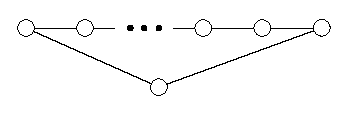
\includegraphics{table1_1(l)} & 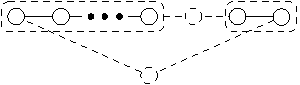
\includegraphics{table1_1(r)}
  \\ \hline
$C_n$ & 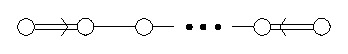
\includegraphics{table1_3(l)} & 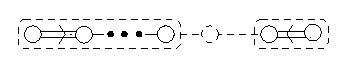
\includegraphics{table1_3(r)}
  \\ \hline
$D_n$ & 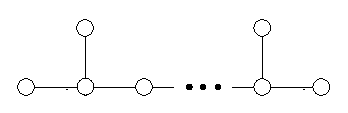
\includegraphics{table1_4(l)} & 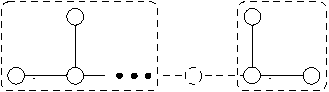
\includegraphics{table1_4(r)}
  \\ \hline
\end{tabular}
}
\caption{Подалгебры $\af,\;\afb$ для классических серий}
\end{table}

В случае серии $B$ ситуация отличается. Причина в том, что в данном случае подалгебра $\afb$ может быть больше, чем результат удаления поддиаграммы  $\af$ и соседних вершин. Подалгебры ортогональной пары $\ \af$ и $\afb$ не обязаны образовывать прямую сумму в $\gf$. Можно явно проверить, что при  $\gf=B_{r}$ и $\af=B_{r_{\af}}$ ортогональная подалгебра -- это $\afb=B_{r-r_{\af}}$. Рассмотрим вложение $B_{r_{\af}}\rightarrow B_{r},\quad 1<r_{\af}<r$. В результате удаления простого корня  $\alpha _{r_{\af}-1}=e_{r_{\af}-1}-e_{r_{\af}}$ расширенная диаграмма Дынкина для $B_{r}$ разбивается на несвязные диаграммы $\af=B_{r_{\af}}$ и $D_{r-r_{\af}}$. Однако корневая система  $\Delta _{\afb}$ содержит не только простые корни  $\left\{ e_{1}-e_{2},e_{2}-e_{3},\ldots ,e_{r_{\af}-2}-e_{r_{\af}-1},e_{1}+e_{2}\right\} $, но и корень $e_{r_{\af}-1}$. То есть  $\Delta _{\afb}$ образует систему типа  $B_{r-r_{\af}}$ и ортогональная пара для вложения $B_{r_{\af}}\rightarrow B_{r}$ -- это  $\left( B_{r_{\af}},B_{r-r_{\af}}\right) $. В следующем разделе мы приводим пример такой ортогональной пары для вложения $B_{2}\rightarrow B_{4}$ (см. Рис. \ref{fig:dynkin}).

Полная классификация регулярных подалгебр аффинных алгебр Ли приведена в недавней работе \cite{1751-8121-41-36-365204}. Из полной классификации максимальных специальных подалгебр классических алгебр Ли \cite{dynkin1952semisimple} мы получаем следующий список пар ортогональных подалгебр $\af,\;\afb$:
\begin{equation*}
\begin{array}{lll}
su(p)\oplus su(q) & \subset su(pq) &  \\
so(p)\oplus so(q) & \subset so(pq) &  \\
sp(2p)\oplus sp(2q) & \subset so(4pq) &  \\
sp(2p)\oplus so(q) & \subset sp(2pq) &  \\
so(p)\oplus so(q) & \subset so(p+q) & \text{для нечетных}\;p\;\text{и}\;q.
\end{array}
\end{equation*}


\subsubsection{Алгоритм рекурсивного вычисления коэффициентов ветвления}

\label{sec:algorithm}

Рекуррентные соотношения (\ref{recurrent-relation}) позволяют нам сформулировать алгоритм для рекурсивного вычисления коэффициентов ветвления. При этом для работы алгоритма не требуется построение модуля $L^{(\mu)}_{\gf}$ или какого-то из модулей $L^{(\nu)}_{\af}$

Алгоритм состоит из следующих шагов:

\begin{enumerate}[(i)]
\item Построить корневую систему $\Delta _{\af}$ для вложения $\af\rightarrow \gf$.

\item Выбрать все положительные корни $\alpha \in \Delta ^{+}$, ортогональные к  $\af$, то есть сформировать множество $\Delta_{\afb }^{+}$.

\item Построить множество $\Gamma _{\af\rightarrow \gf}$. Соотношение  (\ref{eq:142}) определяет знаковую функцию $s(\gamma)$ и множество $\Phi_{\af\subset \gf}$. Вычитание наименьшего веса $\gamma_0$ дает веер вложения (\ref{fan-defined}):
 $\Gamma _{\af\rightarrow \gf}=\left\{ \xi -\gamma _{0}|\xi \in \Phi _{\af\subset \gf}\right\} \setminus \left\{ 0\right\}$.

\item Построить множество $\widehat{\Psi ^{(\mu )}}=\left\{ w (\mu +\rho
)-\rho ;\;w \in W\right\} $ сингулярных весов для  $\gf$-модуля $L^{(\mu )}$.

\item Выбрать веса $\left\{ \mu _{\widetilde{\afb}}\left( w\right) =\pi _{\widetilde{\afb}}\left[ w(\mu +\rho
)-\rho \right] -\mathcal{D}_{\afb}\in \overline{C_{\widetilde{\afb}}}\right\} $. Так как множество  $\Delta_{\afb }^{+}$ фиксировано, легко осуществить проверку принадлежности веса $\mu _{\widetilde{\afb}}\left( w\right) $ к главной камере Вейля $\overline{C_{\widetilde{\afb}}}$ (достаточно вычислить скалярные произведения с фундаментальными весами $\afb^{+}$).

\item Для весов $\mu _{\widetilde{\afb}}\left( w\right) $ вычислить размерности соответствующих модулей, $\mathrm{\dim }\left(L_{\widetilde{\afb}}^{\mu _{\widetilde{\afb}}\left( u\right) }\right) $, используя формулу Вейля для размерностей. Затем построить сингулярный элемент $\Psi ^{\left( \mu \right) }_{\left(  \af, \afb \right)}$.

\item Вычислить сингулярные коэффициенты ветвления используя рекуррентное соотношение (\ref{recurrent-relation}) и выбрать среди них те, которые соответствуют весам в главной камере Вейля $\overline{C_{\af}}$.
\end{enumerate}

Можно ускорить работу алгоритма путем однократного вычисления представителей классов смежности $W/W_{\afb }$.

Следующий раздел состоит из примеров, иллюстрирующих применение данного алгоритма.


\section{Примеры вычисления коэффициентов ветвления модулей конечномерных алгебр Ли}
\label{sec:finite-dimens-lie}

\subsubsection{Регулярное вложение $A_1$ в $B_2$}
\label{sec:regul-embedd-a_1}

Рассмотрим регулярное вложение $A_1\to B_2$. Простые корни $\alpha_1, \alpha_2$ алгебры $B_2$ обозначены пунктирными стрелками на Рисунке \ref{fig:B2_A1}. Мы обозначаем соответствующие элементарные отражения через $w_1, w_2$. Простой корень $\beta = \alpha_1+2\alpha_2$ алгебры $A_1$ показан серым цветом.


\begin{figure}[p]
  \noindent\centering{
    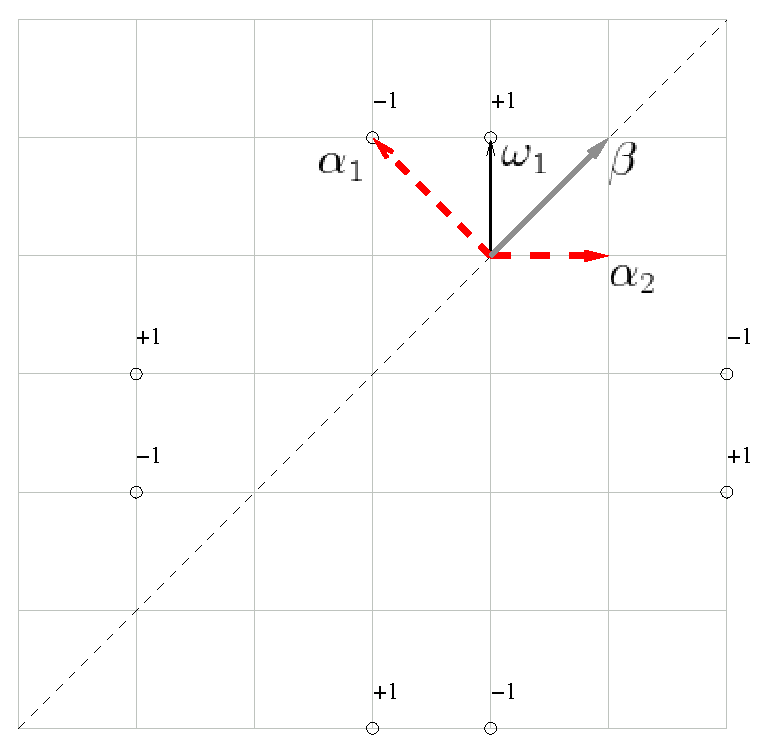
\includegraphics[width=80mm]{figure1}
  }
  \caption{Регулярное вложение  $A_1$ в $B_2$. Простые корни  $\alpha_1, \alpha_2$ алгебры $B_2$ обозначены пунктирными стрелками. Простой корень $\beta = \alpha_1+2\alpha_2$ подалгебры $A_1$ показан серым цветом. Старший вес фундаментального представления $L^{(1,0)=\omega_1}_{B_2}$ выделен черным. Веса сингулярного элемента $\Psi^{(\omega_1)}$ отмечены кругами с подписанными значениями соответствующих определителей $\epsilon(w)$.}
  \label{fig:B2_A1}

%\end{figure}
%\begin{figure}[pb]
  \noindent\centering{
    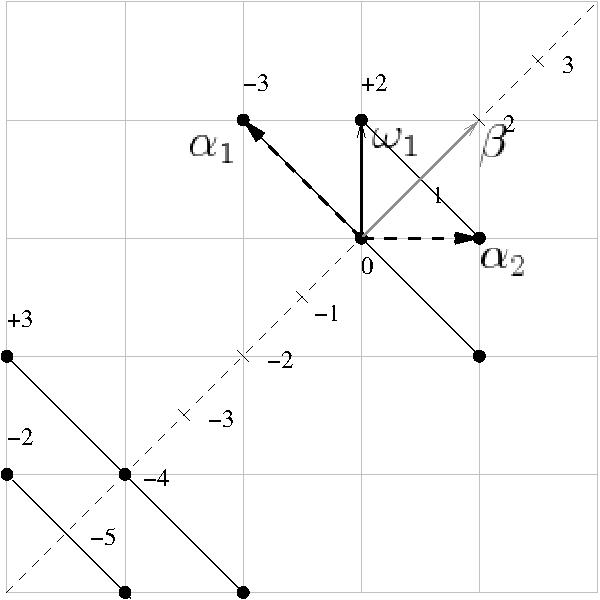
\includegraphics[width=80mm]{figure2}
  }
  \caption{Здесь диаграмма, показанная выше (Рисунок \ref{fig:B2_A1}), дополнена весами $\left( \afb=A_1 \right)$-модулей $L_{\af_{\perp }}^{\mu_{\af_{\perp }}\left( u\right) }$, построенных в точках $\pi _{\af}\left[ u(\mu +\rho )-\rho \right] $ и показанных пунктирными линиями. 
    Подписи к старшим весам   $\mu_{\af_{\perp }}\left( u\right)$ представляют собой значения произведений $\epsilon(u)\dim\left(L_{\afb}^{\mu_{\af_{\perp }}\left( u\right) }\right)$.
    Координаты вдоль корня $\beta$ указаны по отношению к фундаментальному весу $\af$. }
\label{fig:B2_A1_2}
\end{figure}

Выполним редукцию фундаментального представления  $L^{(1,0)=\omega_1}_{B_2}$ ($\omega_1$ -- черная стрелка на Рисунке \ref{fig:B2_A1}) в соответствии с алгоритмом.
Корень $\alpha_1$ ортогонален к $\beta$, так что  $\Delta_{\afb}^+ = \left\{ \alpha_1 \right\}$ (шаг (ii)).
В соответствии с Определением \ref{fan-definition} веер вложения $\Gamma_{A_1\to B_2}$ (шаг (iii)) состоит из двух весов:
\begin{equation*}
  \label{eq:22}
  \Gamma_{A_1\to B_2}=\left\{ (1;2),\; (2;-1) \right\},
\end{equation*}
где вторая компонента -- это значение знаковой функции  $s(\gamma)$.
Сингулярные веса  $\left\{ w (\omega_1 +\rho)-\rho ;\;w \in W\right\}$ (шаг (iv)) показаны кругами с подписанными значениями $\epsilon\left( w \right)$. Пространство  $U$ представляет собой факторпространство $W/W_{\afb}$, где $W_{\afb}=\left\{e,w_1\right\}$. Это означает, что сингулярные веса, находящиеся над прямой, заданной корнем $\beta$, принадлежат главной камере Вейля $\overline{C_{\widetilde{\af_{\perp }}}}$. Из формулы (\ref{defect-perp})  мы получаем  $\mathcal{D}_{\af_{\perp }}=0$ и $\hf_{\perp }=0$, то есть $\left\{ \mu _{\afb}\left( w\right)=\pi _{\afb}\left[ w(\mu +\rho)-\rho \right]\right\}$. Значит есть четыре старших веса для $\af_{\perp }$-модулей.  В базисе фундаментального веса $\frac{1}{2} \alpha_1$ алгебры $\afb$ координаты этих весов
$\left\{ \mu _{\afb}\left( u\right)=\pi _{\afb}\left[ u(\mu +\rho)-\rho \right]| u \in U \right\}$
равны
$\left\{ \left( 1\right) \left( 2\right) \left( 2\right) \left( 1\right) \right\}$ (шаг v).
На Рисунке (\ref{fig:B2_A1_2}) соответствующие весовые диаграммы
$\left\{ \mathcal{N}_{\af_{\perp }}^{\mu _{\af_{\perp }}\left( u\right) }\right\} $
построены из весов $\left\{ \mu _{\af}\left( u\right)\right\} =\left\{\pi _{\af}\left[ u(\mu +\rho )-\rho \right]\right\}
=\left\{ \left( 1\right) \left( 0\right) \left( -4\right) \left( -5\right) \right\}$ подалгебры   $\af$.
В действительности весовые диаграммы нам не нужны, достаточно знать лишь размерности модулей
$L_{\af_{\perp }}^{\mu_{\af_{\perp }}\left( u\right) }$ умноженные на
$\epsilon \left( u\right) $ (шаг vi). Полученные значения должны быть связаны с точками
$\left\{ \left( 1\right) \left( 0\right) \left( -4\right) \left( -5\right) \right\}$ в $P_{\af}$. Сингулярный элемент $\Psi ^{\left( \mu \right) }_{\left(  \af, \afb \right)}$ содержит следующий набор весов и их сингулярных кратностей:
\begin{equation}
  \label{eq:25}
  \left\{(1;2),\; (0;-3),\; (-4;3),\; (-5;-2)\right\}.
\end{equation}

Применяя формулу (\ref{recurrent-relation}) с веером
$\Gamma_{A_1\to B_2}$ к множеству (\ref{eq:25}) (шаг vii)
мы получаем нули для весов больше старшего сингулярного вектора$(1;2)$ и  $k^{(1,0)}_1=2$ для самого вектора $(1;2)$.
Для сингулярного веса $(0;-3)$ на границе $\bar{C}^{(0)}_{\af}$ рекуррентное соотношение дает
\begin{equation*}
  \label{eq:23}
  k^{(1,0)}_{0}=-1\cdot k^{(1,0)}_2 +2\cdot k^{(1,0)}_1 - 3\cdot \delta_{0,0} = 1,
\end{equation*}
и редукция завершена: $L_{B_2\downarrow A_1}^{\omega_1}=
2L_{A_1}^{\omega_{\left(A_1\right)} }
\bigoplus
L_{A_1}^{2\omega_{\left(A_1\right)} }$.

\subsubsection{Вложение  $B_2$ в $B_4$}
\label{sec:someth-high-dimens}
Рассмотрим регулярное вложение $B_2 \rightarrow B_4$. Соответствующие диаграммы Дынкина показаны на Рисунке \ref{fig:dynkin}.
\begin{figure}[h]
  \centering
  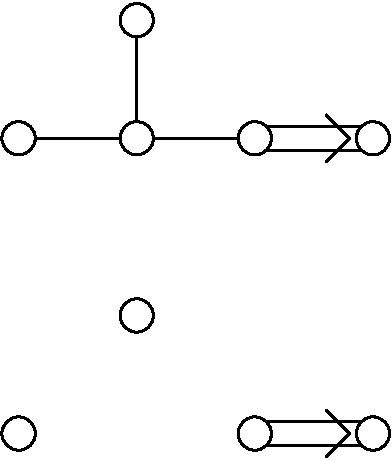
\includegraphics[width=60mm]{figure3}
  \caption{Регулярное вложение  $B_2 \rightarrow B_4$ получается путем исключения вершины из диаграммы Дынкина. 
    Напомним, что в данном случае $\afb$ равна $B_2$, тогда как на диаграмме видна только подалгебра $A_1\oplus A_1$ (см. раздел \ref{sect-embeddings}).}
  \label{fig:dynkin}
\end{figure}

\begin{figure}[pt]
  \centering
    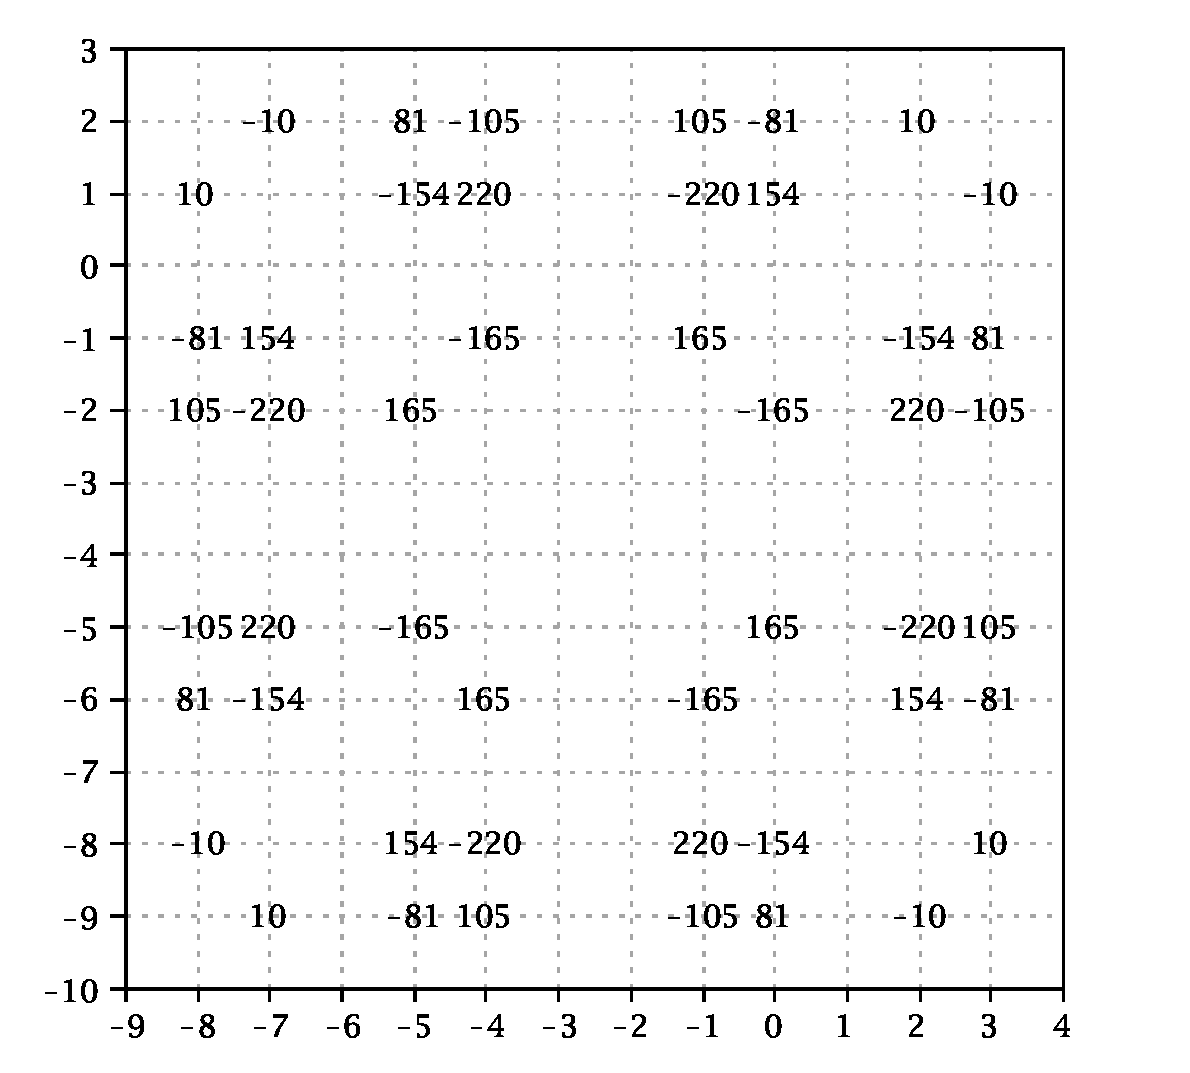
\includegraphics[width=100mm,height=90mm]{figure4}
  \caption{Сингулярный элемент  $e^{\gamma_0}\Psi ^{\left( \mu \right) }_{\left(  \af, \afb \right)}$ показан в весовом подпространстве $P_{\af}$, где $\af=B_2$ и базис равен $\left\{e_3,e_4\right\}$. Показаны спроектированные сингулярные веса $\left\{\pi _{\af}\left[ u(\mu +\rho )-\rho \right] +\gamma_0 | u \in U \right\}$, сдвинутые на  $\gamma_0$ и снабженные множителям  $\epsilon(u)\dim\left(L_{\af_{\perp }}^{\mu_{\af_{\perp }}\left( u\right) }\right)$.}
  \label{fig:B4B2anom}

%\end{figure}
%
%\begin{figure}[pb]
  \centering
  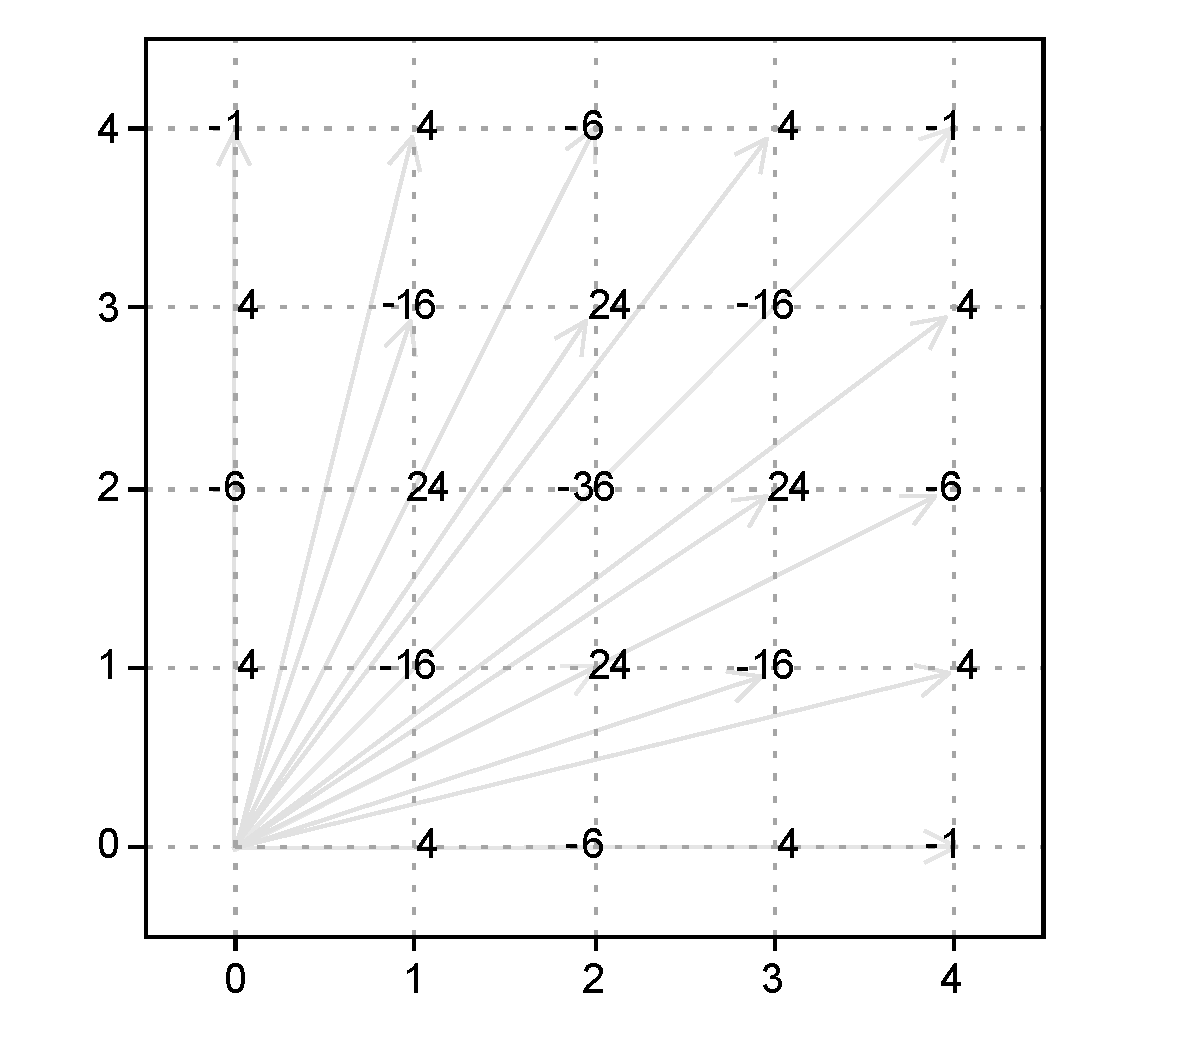
\includegraphics[height=80mm]{figure5}
  \caption{Веер $\Gamma$ для вложения $B_2\rightarrow B_4$ со значениями функции $s(\gamma+\gamma_0)$, указанными при соответствующих весах $\gamma \in \Gamma$.}
  \label{fig:B4B2Fan}
\end{figure}

В ортогональном базисе $\left\{e_1,\dots,e_4\right\}$ простые и положительные корни алгебры $B_4$ равны
\begin{eqnarray*}
  \label{eq:19}
  S_{B_4}= \{e_1 - e_2,\; e_2 - e_3,\; e_3 - e_4,\; e_4\},\\[2mm]
 \Delta^+_{B_4}=\left\{ (e_1 - e_2,\; e_2 - e_3,\; e_3 - e_4,\; e_4,\; e_1 - e_3,\; e_2 - e_4,\; e_3 + e_4,\; e_3,\; e_1 - e_4,\;\right.\\
 \left. e_2 + e_4,\; e_2,\; e_1 + e_4,\; e_2 + e_3,\; e_1,\; e_1 + e_3,\; e_1 + e_2\right\}
\end{eqnarray*}
Подалгебра  $\af=B_2$ задается простыми корнями
\begin{equation*}
  \label{eq:155}
 S_{B_2}=\{e_3-e_4,e_4\}.
\end{equation*}
Ее ортогональный партнер $\afb=B_2$ определяется корнями
\begin{eqnarray*}
  \label{eq:27}
  S_{\afb}=\{e_1-e_2,e_2\},\\
 \Delta^{+}_{\afb}= \left\{e_1-e_2,e_1+e_2,e_1,e_2\right\}.
\end{eqnarray*}
После определения множества $\Delta^+_{B_4} \setminus  \Delta^{+}_{\afb}$ можно построить веер вложения $\Gamma_{B_2 \to B_4}$ применяя Определение \ref{fan-definition}. Так как для этого вложения $s\left( \gamma_0\right)=-1$, в рекуррентном соотношении нам нужен только множитель $s\left(\gamma + \gamma_0\right)$. Результат построения веера показан на Рисунке \ref{fig:B4B2Fan}.

Рассмотрим модуль $L^{\mu}$ алгебры  $B_4$ со старшим весом $\mu=2e_1 + 2 e_2 + e_3 + e_4$; \,
$\mathrm{dim}(L^{\left[0,1,0,2\right]})=2772$.
В данном случае дефект не равен нулю, $\mathcal{D}_{\af_{\perp }}=-2\left( e_1 + e_2 \right)$, тогда как $\hf_{\bot}$ тривиальна. Среди сингулярных весов есть 
48 векторов со свойством $\left\{ \mu _{\afb}\left( u\right) =\pi _{\af_{\perp }}\left[ u(\mu +\rho)-\rho \right] -\mathcal{D}_{\afb}\in \overline{C_{\afb}}\right\} $.
Таким образом мы определили множество $U=\left\{ u \right\}$. Вычислим размерности соответствующих  $\afb$-модулей со старшими весами $\mu_{\afb}\left( u\right)$ (используем формулу Вейля для размерностей) и умножим их на $\epsilon\left( u \right)$. В результате получим сингулярный элемент
$\Psi ^{\left( \mu \right) }_{\left(  \af, \afb \right)}$, показанный на Рисунке \ref{fig:B4B2anom}.

Теперь поместим веер  $\Gamma$ (см. Рисунок \ref{fig:B4B2Fan}) в старший из весов, показанных на Рисунке \ref{fig:B4B2anom} и проведем рекурсивное вычисление коэффициентов ветвления (с использованием соотношения (\ref{recurrent-relation})):
\begin{eqnarray*}
  \label{eq:24}
  \pi_{\af} \left(ch L^{\left[0,1,0,2\right]}_{B_4}\right) = 6 \; ch L^{\left[0,0\right]}_{B_2}+ 60
  \; ch L_{B_2}^{\left[0,2\right]}+ 30 \; ch L_{B_2}^{\left[1,0\right]}+ 19 \; ch L_{B_2}^{\left[2,0\right]}+\\
  40 \; ch L_{B_2}^{\left[1,2\right]}+ 10 \; ch L_{B_2}^{\left[0,4\right]}.
\end{eqnarray*}

\section{Преимущества рекуррентного алгоритма для коэффициентов ветвления}
\label{sec:branching-algor-comparison}

При вычислении коэффициентов ветвления использование формулы Фрейденталя требует полного построения формальных характеров представления алгебры и всех представлений подалгебры, входящих в его разложение. Такой подход становится непрактичным для большого ранга алгебры и подалгебры, например, при максимальных вложениях. 

Альтернативный алгоритм описан в разделе \ref{sec:algorithm}. Рассмотренный там же пример регулярного вложения \ref{sec:someth-high-dimens}  $B_{2}\subset B_{4}$ позволяет сделать следующее сравнение числа требующихся операций. В данном примере веер вложения состоит из 24 элементов. Для разложения модуля алгебры  $B_{4}$ необходимо построить подмножество сингулярных весов модуля, проектирующихся в главную камеру Вейля подалгебры $B_{2}$. Полное множество сингулярных весов состоит из 384 элементов, в главную камеру Вейля проектируется не более 48, так что время на построение этого множества пренебрежимо мало, если число коэффициентов ветвления более 48. Мы можем оценить сверху общее число операций для вычисления коэффициентов ветвления произведением числа весов в главной камере Вейля подалгебры с ненулевыми коэффициентами ветвления на число элементов веера вложения. 
С другой стороны, при использовании алгоритма, основанного на построении всех характеров при помощи формулы Фрейденталя мы должны вычислить кратности для каждого модуля в разложении, так что общее количество операций растет с ростом числа весов в представлении быстрее, чем квадрат числа весов в главной камере Вейля подалгебры с ненулевыми коэффициентами ветвления. 

Чтобы проиллюстрировать эту разницу в производительности алгоритмов, мы приводим Рисунок \ref{fig:branching}, на котором показано время, необходимое для вычисления коэффициентов ветвления для вложения $B_{3}\subset B_{4}$.

\begin{figure}[h]
  \noindent\centering{
   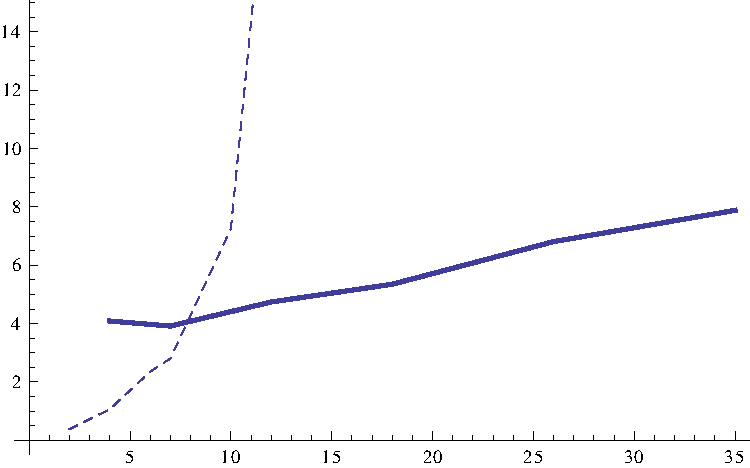
\includegraphics[width=100mm]{figures/branching-timing}
  }
  \caption{Время работы алгоритмов, основанных на применении формулы Фрейденталя \eqref{eq:15} (пунктиром)  и рекуррентного соотношения \eqref{recurrent-relation} (сплошная линия) с ростом числа весов в  $\bar C$ при вычислении коэффициентов ветвления для вложения $B_{3}\subset B_{4}$.}
  \label{fig:branching}
\end{figure}

%\newpage
\section{Примеры приложений в конформной теории поля}
\label{sec:phys-appl}

\subsubsection{Конформные вложения}
\label{sec:conformal-embeddings}

Как мы уже объясняли в разделе \ref{sec:modular-invariance}, коэффициенты ветвления для вложения аффинной алгебры Ли в аффинную алгебру Ли можно использовать для построения модулярно-инвариантной статсуммы для моделей Весса-Зумино-Новикова-Виттена в двумерной конформной теории поля (\cite{difrancesco1997cft}, \cite{Walton:1999xc}, \cite{walton1989conformal}, \cite{schellekens1986conformal}).
В этих моделях аффинные алгебры Ли являются алгебрами токов. 

Модулярная инвариантность статсуммы необходима для самосогласованности теории на торе и римановых поверхностях высшего рода, что важно для приложений конформной теории поля в теории струн и описании критического поведения.

Отметим, что случай конформных вложений довольно специфичен. Если рассмотреть соотношение (\ref{eq:153}) и асимптотику функций ветвления, то можно доказать теорему о конечной приводимости \cite{kac1988modular}. Она утверждает, что для конформного вложения  $\af\longrightarrow\mathfrak{g}$ лишь конечное число коэффициентов ветвления отлично от нуля. Кроме того, верно следующее замечание. 

\begin{mynote} Ортогональная подалгебра  $\afb$ всегда тривиальна в случае конформного вложения $\af\longrightarrow \mathfrak{g}$.
\begin{proof}
Рассмотрим разложение тензора энергии-импульса на моды:
\begin{equation*}
\label{eq:47}
  T(z)=\frac{1}{2(k+h^v)}\sum_n z^{-n-1}L_n.
\end{equation*}
Моды $L_n$ представляют собой комбинации нормально упорядоченных произведений генераторов алгебры $\gf$,
\begin{equation*}
\label{eq:48}
  L_n=\frac{1}{2(k+h^v)}\sum_{\alpha}\sum_m:J^{\alpha}_m J^{\alpha}_{n-m}: \; .
\end{equation*}
При конформном вложении тензоры энергии-импульса  $T_{\mathfrak{g}}(z)$ и $T_{\af}(z)$ равны (см. (\ref{eq:127})).

В эти комбинации мы должны подставить генераторы подалгебры $\af$ выраженные через генераторы $\mathfrak{g}$ и получить тензор энергии-импульса $T_{\mathfrak{g}}$. Но если набор генераторов, связанных с  $\Delta_{\afb}$ не пуст, это невозможно, так как  $T_{\mathfrak{g}}$ содержит генераторы $J^{\alpha}_n$, где $\alpha\in \Delta_{\afb}$.
\end{proof}
\end{mynote}



\subsubsection{Специальное вложение $\hat{A}_1\rightarrow\hat{A}_2$.}
\label{sec:spec-embedd-hata_1s}
Рассмотрим следующий пример конформного вложения  аффинной подалгебры $\af$ в  аффинную алгебру Ли $\gf$. Вложение $\hat{A}_1 \rightarrow \hat{A}_2$ является аффинным расширением специального вложения $A_1 \rightarrow A_2$ с индексом вложения $x_e=4$. Так как мы должны рассматривать $\gf$-модули уровня один, соответствующие  $\af$-модули будут иметь уровень $\tilde{k}=kx_e=4$.

Существует три фундаментальных веса алгебры  $\hat{A}_2$ имеющих уровень один. 
Легко видеть, что множество $\Delta_{ \afb }$ пусто и подалгебра $\afb=0$. Тогда ${\cal D}_{\afb}=0$, $\hf_{\perp}$ -- одномерная абелева подалгебра и размерность $\tilde\afb=\afb\oplus \hf_{\perp}$ также равна 1. Удобно выбрать классический корень для подалгебры $\hat{A}_1$ равным $\beta=\frac{1}{2}(\alpha_1+\alpha_2)$.

Используем Определение (\ref{fan-definition}) и построим веер $\Gamma_{\hat A_1\to\hat A_2}$. В этом случае $\gamma_0 =0$ и знак  $s\left( 0 \right)=-1$, то есть мы используем знаковую функцию $s(\gamma)$ (см. Рисунок \ref{fig:AffineA2A1Fan}).


\begin{figure}[h!bt]
  \centering
  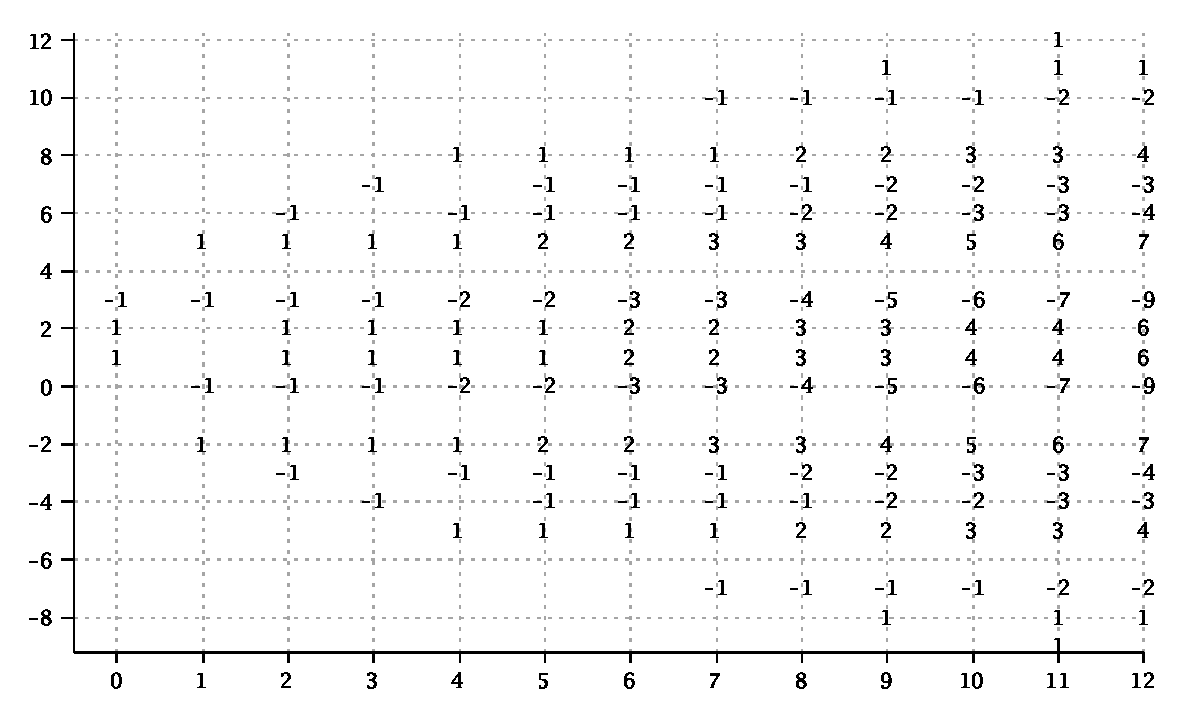
\includegraphics[width=125mm]{figure6}

  \caption{Веер  $\Gamma_{\hat{A_1}\rightarrow \hat{A_2}}$ для вложения $\hat{A_1}\rightarrow \hat{A_2}$ в базисе $\left\{\beta,\delta \right\}$. Заметим, что  $\gamma_0 =0$ и значения $s(\gamma)$ приписаны к весам $\gamma\in \Gamma_{\hat{A_1}\rightarrow \hat{A_2}}$}
  \label{fig:AffineA2A1Fan}
\end{figure}

Рассмотрим модуль $L^{\omega_0=(0,0;1;0)}$. Здесь мы используем обозначение (конечномерная часть; уровень; грейд)
для старшего веса и координаты конечномерной части даются индексами Дынкина (см. раздел \ref{sec:weights-roots}).

Множество весов $\widehat{\Psi^{(\omega_0)}}$ показано на Рисунке \ref{fig:affine_A2_anom_point} вплоть до шестого грейда.

\begin{figure}[h!tb]
  \hspace*{-1.5cm}
  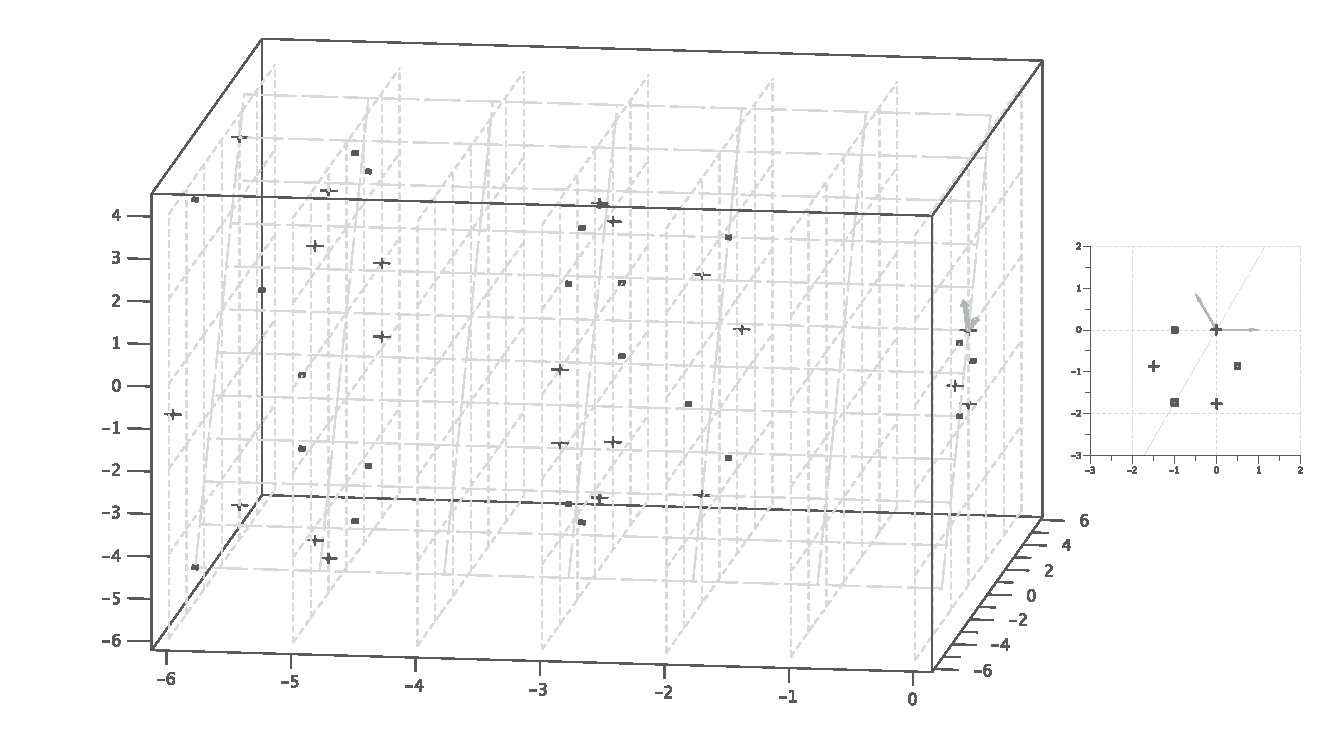
\includegraphics[width=180mm]{figure7}
  \caption{Сингулярные веса модуля $L_{\hat{A_2}}^{\omega_0}=L^{(0,0;1;0)}_{\hat{A_2}}$. Классическое сечение (нулевой грейд) диаграммы показано отдельно в правой части рисунка. 
    Мы используем ортогональный базис с единичным вектором, равным $\alpha_1$. Веса $w (\omega_0+\rho)-\rho$ показаны крестами, если $\epsilon(w)=1$ и квадратами при $\epsilon(w)=-1$. Простые корни классической подалгебры  $A_2$ показаны серым, а диагональная плоскость соответствует подалгебре Картана вложенной алгебры $\hat{A}_1$.}
  \label{fig:affine_A2_anom_point}
\end{figure}

Следующий шаг состоит в проектировании сингулярных весов на $P_{\hat A_1}$. В результате получается элемент $\Psi ^{\left( \omega_0 \right) }_{\left(  \hat A_1\, , \, \afb=0 \right)}$, изображенный на Рисунке \ref{fig:AffineA2_A1_anom_proj} вплоть до двенадцатого грейда.
\begin{figure}[h!tb]
  \centering
  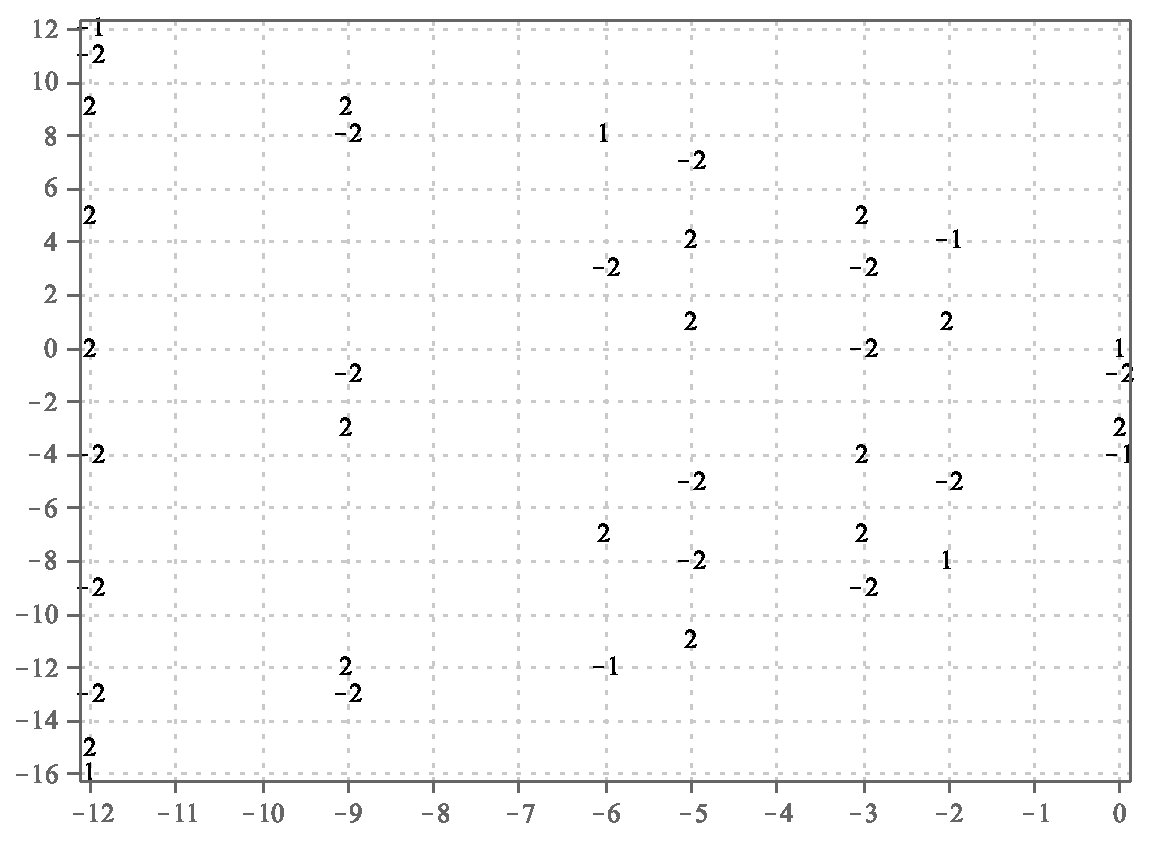
\includegraphics[width=130mm]{figure8}
  \caption{Сингулярный элемент $\Psi ^{\left( \omega_0 \right) }_{\left(  \hat A_1\, , \, \afb=0 \right)}$ показан в $P_{\hat A_1}$ с базисом $\left\{\beta,\delta \right\}$.}
  \label{fig:AffineA2_A1_anom_proj}
\end{figure}

Используя рекуррентное соотношение  (\ref{recurrent-relation}) с веером
$\Gamma_{\hat{A_1}\rightarrow \hat{A_2}}$ и сингулярными весами $\Psi ^{\left( \omega_0 \right) }_{\left(  \hat A_1\, , \, \afb=0 \right)}$, мы получаем сингулярные коэффициенты ветвления, показанные на Рисунке \ref{fig:AffineA2_A1_branching}.
\begin{figure}[h!tb]
  \centering
  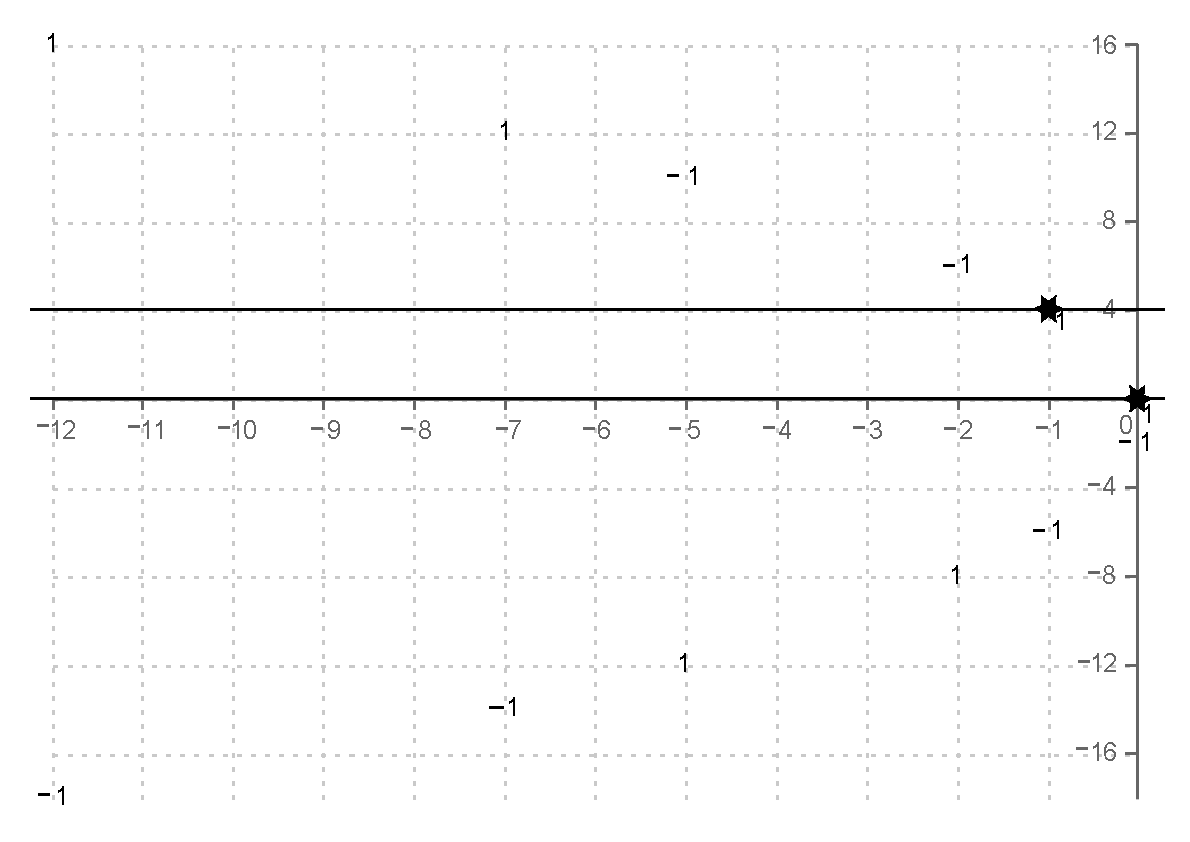
\includegraphics[width=130mm]{figure9}
  \caption{Сингулярные коэффициенты ветвления для вложения $\hat{A_1}\subset \hat{A_2}$. Границы главной камеры Вейля $\bar{C}_{\hat{A}_1}$ показаны черными линиями. Два сингулярных веса, расположенные в главной камере Вейля, отмечены звездочками. Они оба имеют кратность 1, то есть соответствующие коэффициенты ветвления равны 1.}
  \label{fig:AffineA2_A1_branching}
\end{figure}
Внутри камеры Вейля $\bar{C}_{\hat{A}_1}$ (ее границы показаны на Рисунке \ref{fig:AffineA2_A1_branching}) находятся только два ненулевых сингулярных веса и оба они имеют кратность 1. Это старшие веса подмодулей $\af$ и их кратности равны коэффициентам ветвления. То есть мы получаем разложение
\begin{equation*}
  \label{eq:43}
  L^{(0,0;1;0)}_{\hat{A_2}\downarrow \hat{A_1}}= L_{\hat{A_1}}^{(0;4;0)}\oplus L_{\hat{A_1}}^{(4;4;0)}.
\end{equation*}
Заметим, что теорема о конечной приводимости выполняется.

Тот же веер $\Gamma_{\hat{A_1}\rightarrow \hat{A_2}}$ можно использовать для других модулей старшего веса $L^{\mu}_{\hat{A_2}}$. В частности для неприводимых модулей уровня один мы получаем тривиальное ветвление:
\begin{eqnarray*}
  \label{eq:44}
   L^{(1,0;1;0)}_{\hat{A_2}\downarrow \hat{A_1}}= L_{\hat{A_1}}^{(2;4;0)},\\
   L^{(0,1;1;0)}_{\hat{A_2}\downarrow \hat{A_1}}= L_{\hat{A_1}}^{(2;4;0)}.
\end{eqnarray*}

Используя эти результаты легко получить модулярно-инвариантную статсумму:
\begin{equation*}
  \label{eq:45}
  Z=\left|\chi_{(4;4;0)}+\chi_{(0;4;0)}\right|^2+2\chi_{(2;4;0)}^2.
\end{equation*}

\subsubsection{Coset-модели}
\label{sec:coset-models}

Coset-модели \cite{Goddard198588}, тесно связанные с калибровочными ВЗНВ-моделями, активно изучаются в теории струн, особенно в струнных моделях в пространстве анти де Ситтера
\cite{Maldacena:2000hw,Maldacena:2000kv,Maldacena:2001km,Maldacena:2001ky,Aharony:1999ti}. Характеры в coset-моделях пропорциональны функциям ветвления.
\begin{equation}
  \label{eq:31}
  \chi^{(\mu)}_{\nu}(\tau)=e^{2\pi i \tau (m_{\mu}-m_{\nu})} b^{(\mu)}_{\nu}(\tau),
\end{equation}
где
\begin{equation*}
  \label{eq:46}
  m_{\mu}=\frac{\left|\mu+\rho\right|^2}{2(k+g)}-\frac{\left|\rho\right|^2}{2g}.
\end{equation*}
Проблема построения функций ветвления для  coset-моделей рассматривалась в работах  \cite{Dunbar:1992gh}, \cite{Hwang:1994yr}, \cite{lu1994branching}.

Вернемся к нашему примеру \ref{sec:regul-embedd-a_1} и рассмотрим аффинное расширение вложения $A_1 \rightarrow B_2$. Так как вложение регулярно и индекс $x_e=1$, модули подалгебры и исходный модуль имеют одинаковый уровень. Множество положительных корней с нулевой проекцией на корневое пространство подалгебры  $\hat{A_1}$ то же, что и в конечномерном случае: $\Delta^{+}_{\afb}=\left\{ \alpha_1 \right\}$ и $\afb=A_1$. Легко видеть, что здесь $\hf_{\perp}$ тривиальна и  ${\cal D}_{\afb}=0$.

Используя Определение \ref{fan-definition} мы получаем веер вложения $\Gamma_{\hat{A_1} \longrightarrow  \hat{B_2} }$. Заметим, что наименьший вес веера $\gamma_0$ равен нулю и  $s\left( \gamma_0 \right)=-1$. Значения знаковой функции  $s(\gamma)$ для $ \gamma \in \Gamma_{\hat{A_1} \longrightarrow  \hat{B_2} }$ показаны на Рисунке \ref{fig:AffineB2A1Fan}.
Мы ограничили вычисление двенадцатым грейдом. 
\begin{figure}[h!bt]
  \centering
  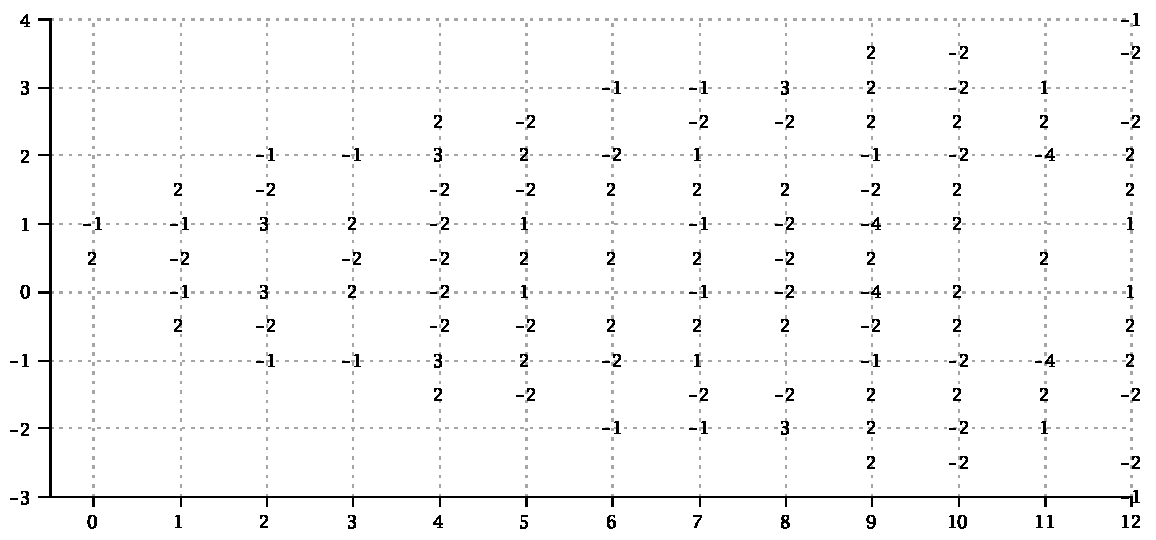
\includegraphics[width=135mm]{figure10}
  \caption{Веер $\Gamma_{\hat{A_1}\rightarrow \hat{B_2}}$ для вложения $\hat{A_1}\rightarrow \hat{B_2}$ в базисе $\left\{\beta,\delta \right\}$. Значения $s(\gamma)$ показаны для весов $\gamma\in \Gamma_{\hat{A_1}\rightarrow \hat{B_2}}$}
  \label{fig:AffineB2A1Fan}
\end{figure}

Рассмотрим модуль уровня один $L^{\left( 1,0;1;0 \right)}_{\hat{B_2}}$  со старшим весом  $\omega_1=(1,0;1;0)$, где координаты конечномерной части даны в ортогональном базисе $e_1,e_2$. Множество сингулярных весов для этого модуля вплоть до шестого грейда приведено на Рисунке \ref{fig:affine_B2_anom_point}.

\begin{figure}[h!tb]
%  \hspace*{-2cm}
  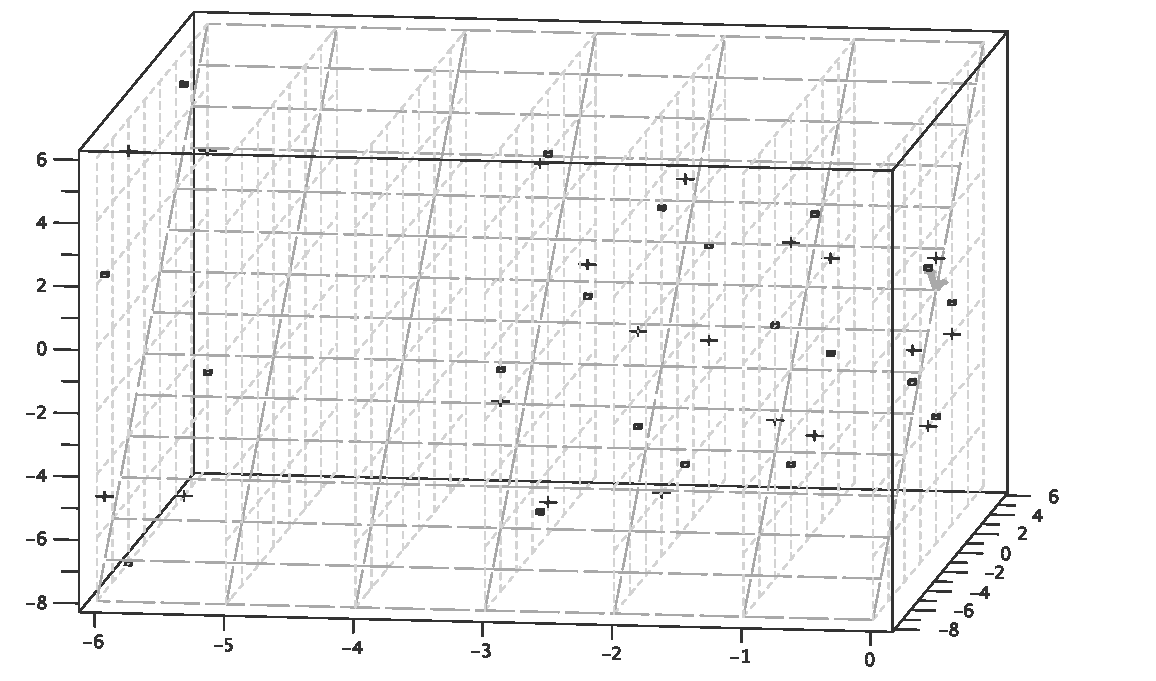
\includegraphics[width=140mm]{figure11}
  \caption{Сингулярные веса модуля $L^{(1,0;1;0)}_{\hat B_2 }$. В классическом сечении используется стандартный базис  $\{e_1,e_2\}$. Веса в нулевом грейде те же, что и на Рисунке \ref{fig:B2_A1}. Веса  $w (\omega_1+\rho)-\rho$ отмечены крестами, если $\epsilon(w)=1$ и квадратами при $\epsilon(w)=-1$. Простые корни классической подалгебры  $B_2$ показаны серым, а диагональная плоскость соответствует подалгебре Картана вложенной алгебры $\hat{A}_1$.}
  \label{fig:affine_B2_anom_point}
\end{figure}

В соответствии с рекурсивным алгоритмом  \ref{sec:algorithm} мы проектируем сингулярные веса на $P_{\hat{A_1}}$ и вычисляем размерности $\afb$-модулей $L^{\pi_{\afb}(w(\mu+\rho))-\rho_{\afb}}_{\afb}$. В нулевом грейде эта проекция дает в точности множество $\Psi ^{\left( \mu \right) }_{\left(  A_1, A_1 \right)}$, соответствующее вложению классической алгебры Ли  $A_1\rightarrow B_2$. Это можно заметить сравнивая Рисунок \ref{fig:B2_A1} и Рисунок \ref{fig:AffineB2_A1_anom_proj}, на котором сингулярный элемент $\Psi ^{\left( \mu \right) }_{\left(  \widehat{A_1}, A_1 \right)}$ для аффинного вложения  $\hat{A_1}\to\hat{B_{2}}$  показан вплоть до двенадцатого грейда. Кратности старших весов внутри главной камеры Вейля
$\bar{C}^{\left( 0 \right)}_{\hat{A_1}}$ определяют следующие значения коэффициентов ветвления (до двенадцатого грейда):
\begin{eqnarray*}
  \label{eq:28}
  L^{\omega_1}_{\hat{B_2}\downarrow \hat{A_1}}
  &=&2 L_{\hat{A_1}}^{\omega_1}\oplus 1 L_{\hat{A_1}}^{\omega_0}\oplus 4 L_{\hat{A_1}}^{\omega_0-\delta}\oplus\\
    &&2 L_{\hat{A_1}}^{\omega_1-\delta}\oplus 8 L_{\hat{A_1}}^{\omega_0-2\delta}\oplus
    8 L_{\hat{A_1}}^{\omega_1-2\delta}\oplus 15 L_{\hat{A_1}}^{\omega_0-3\delta}\oplus\\
    &&12 L_{\hat{A_1}}^{\omega_1-3\delta}\oplus 26 L_{\hat{A_1}}^{\omega_1-4\delta}\oplus
    29 L_{\hat{A_1}}^{\omega_0-4\delta}\oplus 51 L_{\hat{A_1}}^{\omega_0-5\delta}\oplus\\
    &&42 L_{\hat{A_1}}^{\omega_1-5\delta}\oplus 78 L_{\hat{A_1}}^{\omega_1-6\delta}\oplus
    85 L_{\hat{A_1}}^{\omega_0-6\delta}\oplus 120 L_{\hat{A_1}}^{\omega_1-7\delta}\oplus\\
    &&139 L_{\hat{A_1}}^{\omega_0-7\delta}\oplus 202 L_{\hat{A_1}}^{\omega_1-8\delta}\oplus
    222 L_{\hat{A_1}}^{\omega_0-8\delta}\oplus 306 L_{\hat{A_1}}^{\omega_1-9\delta}\oplus\\
    &&346 L_{\hat{A_1}}^{\omega_0-9\delta}\oplus 530 L_{\hat{A_1}}^{\omega_0-10\delta}\oplus
    482 L_{\hat{A_1}}^{\omega_1-10\delta}\oplus 714 L_{\hat{A_1}}^{\omega_1-11\delta}\oplus\\
    &&797 L_{\hat{A_1}}^{\omega_0-11\delta}\oplus 1080 L_{\hat{A_1}}^{\omega_1-12\delta}\oplus
    1180 L_{\hat{A_1}}^{\omega_0-12\delta}\oplus \dots
\end{eqnarray*}
\begin{figure}[h!tb]
  \centering
  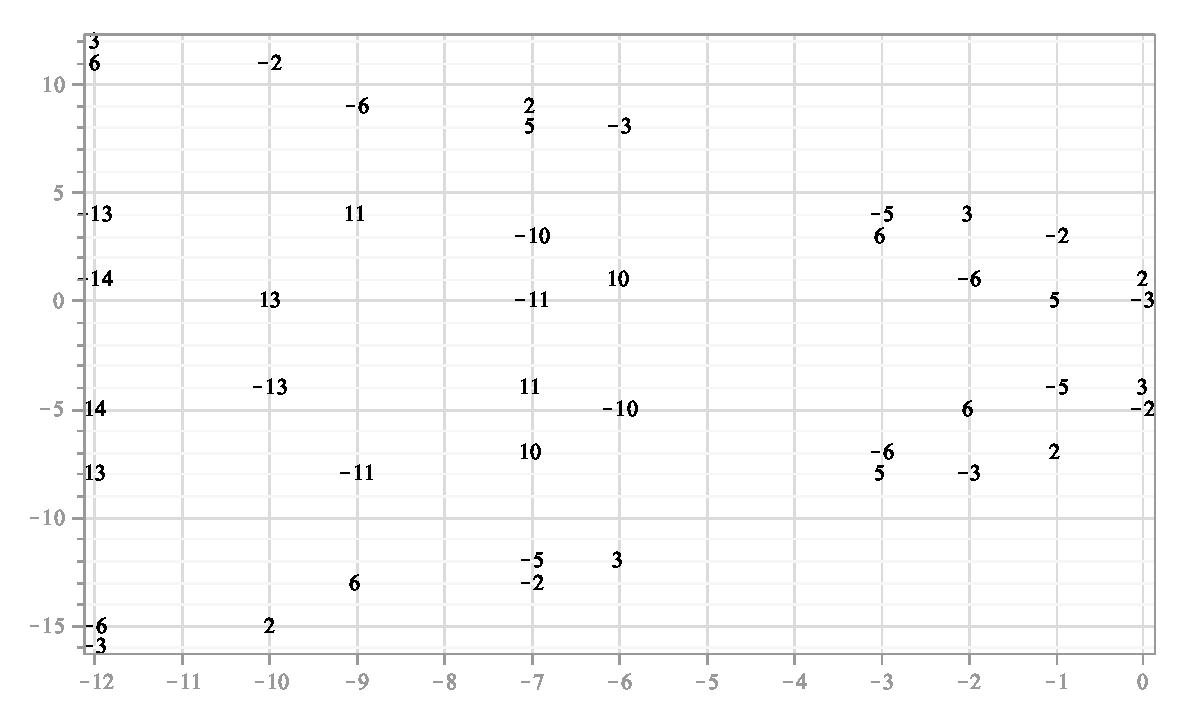
\includegraphics[width=120mm]{figure12}
  \caption{Сингулярный элемент $\Psi ^{\left( \omega_1 \right) }_{\left(  \widehat{A_1}, A_1 \right)}$ в базисе $\{\beta,\delta\}$. Размерности соответствующих  $\afb=A_1$-модулей со знаками  $\epsilon(u)$ представлены на рисунке.}
  \label{fig:AffineB2_A1_anom_proj}
\end{figure}

\begin{figure}[tb]
  \centering
  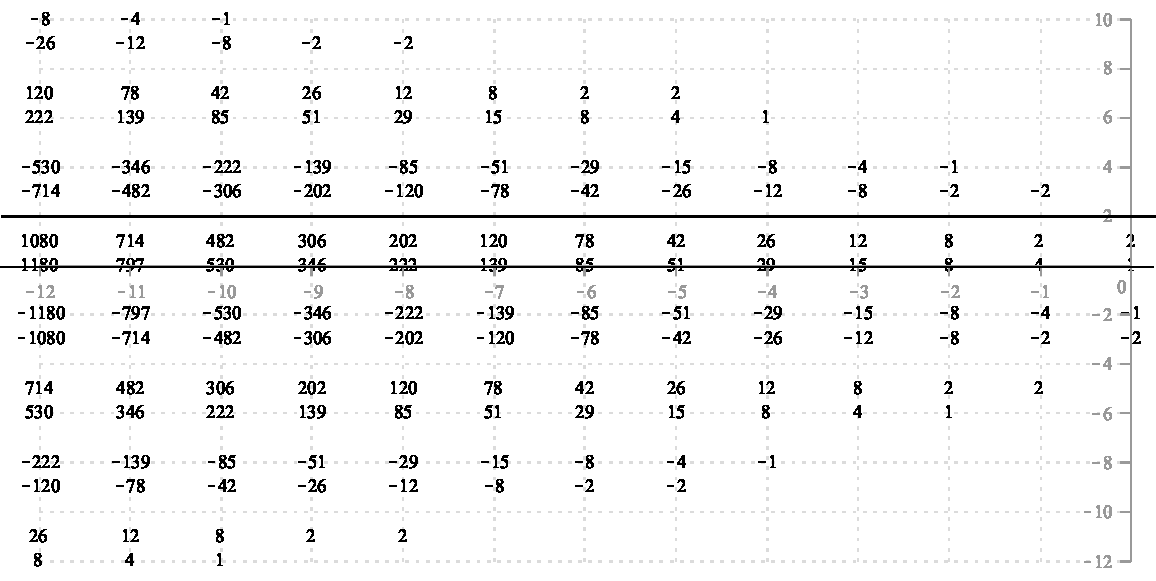
\includegraphics[width=120mm]{figure13}
  \caption{Сингулярные коэффициенты ветвления для вложения $\hat{A_1}\rightarrow \hat{B_2}$. Использован базис $\{\beta,\delta\}$. Границы главной камеры Вейля $\bar{C}_{\hat{A}_1}$ показаны черными линиями. Сингулярные коэффициенты ветвления внутри главной камеры Вейля равны коэффициентам ветвления для вложения $\hat{A_1}\rightarrow \hat{B_2}$.}
  \label{fig:AffineB2_A1_branching}
\end{figure}

Этот результат можно представить в виде набора функций ветвления:
\begin{eqnarray*}
  \label{eq:29}
  \begin{array}{cc}
    b^{(\omega_1)}_{0}= & 1 + 4\,q^{1}+ 8\,q^{2}+ 15\,q^{3}+ 29\,q^{4}+ 51\,q^{5}+ 85\,q^{6}+ 139\,q^{7}+\\
     &222\,q^{8}+ 346\,q^{9}+ 530\,q^{10}+ 797\,q^{11}+ 1180\,q^{12}+\dots\\
  \end{array}\\
  \begin{array}{cc}
    b^{(\omega_1)}_{1}= &2+2\,q^{1}+8\,q^{2}+12\,q^{3}+26\,q^{4}+42\,q^{5}+78\,q^{6}+120\,q^{7}+\\
    & 202\,q^{8}+306\,q^{9}+482\,q^{10}+714\,q^{11}+1080\,q^{12}+\dots
  \end{array}
\end{eqnarray*}
Здесь $q=\exp (2\pi i \tau)$ и нижний индекс нумерует функции ветвления по их старшим весам в  $P^+_{\hat{A_1}}$, равным фундаментальным весам $\omega_0=\lambda_0=(0,1,0),\; \omega_1=\alpha/2=(1,1,0)$.

Теперь мы можем вернуться к равенству (\ref{eq:31}) и получить выражение для характеров coset-модели $B_2/A_1$:
\begin{equation*}
  \label{eq:35}
  \begin{array}{cc}
    \chi^{(\omega_1)}_{1}(q)= & q^{\frac{7}{12}}\left( 2+2\,q^{1}+8\,q^{2}+12\,q^{3}+26\,q^{4}+42\,q^{5}+78\,q^{6}+120\,q^{7}+\right. \\
    & \left. 202\,q^{8}+306\,q^{9}+482\,q^{10}+714\,q^{11}+1080\,q^{12}+\dots \right),\\
    \chi^{(\omega_1)}_{0}(q) = & q^{\frac{5}{6}}\left(1 + 4\,q^{1}+ 8\,q^{2}+ 15\,q^{3}+ 29\,q^{4}+ 51\,q^{5}+ 85\,q^{6}+ 139\,q^{7}+\right. \\
    &\left. 222\,q^{8}+ 346\,q^{9}+ 530\,q^{10}+ 797\,q^{11}+ 1180\,q^{12}+\dots\right).
  \end{array}
\end{equation*}

\section{Заключение}
\label{sec:conclusion}

Мы продемонстрировали, что техника веера вложения может использоваться для работы с произвольными редуктивными подалгебрами (как максимальными, так и не максимальными). Также показано, что проблема редукции для  $\af \subset \gf$ тесно связана со свойствами ортогонального партнера $ \afb $ подалгебры $\af$. Подалгебра  $\afb$ соответствует подмножеству положительных корней $\Delta^{+}_{\afb}$ в $\Delta_{\mathfrak{g}}^{+}$, которое тривиализует подалгебру Картана $\hf_{\afb}$. Веер вложения и множества сингулярных весов для модулей старшего веса алгебры $\gf$ существенным образом зависят от структуры  $\afb$ и ее подмодулей.  Для веера  $\Gamma_{\af\rightarrow \gf}$ эта зависимость почти очевидна: в элементе  $\Phi_{\af\rightarrow \gf}$ исключены множители, соответствующие корням  $\Delta^{+}_{\afb}$. Преобразование множества спроектированных сингулярных весов более интересно. Мы показали, что в новом сингулярном элементе $\Psi ^{\left( \mu \right) }_{\left(  \af, \afb \right)}$ коэффициенты зависят от $\afb$-подмодулей (их старшие веса $\mu _{\widetilde{\afb}}\left( u\right)$ заданы вложением и весами первоначального элемента $\Psi^{\mu}$). К счастью, для вычислений не требуется никакой информации о  $L^{\mu _{\widetilde{\afb}}\left( u\right)}_{\left\{ \afb \right\}}$-подмодулях, кроме их размерностей. В новом сингулярном элементе $\Psi ^{\left( \mu \right) }_{\left(  \af, \afb \right)}$ кратности весов равны размерностям $\dim\left(L^{\mu _{\widetilde{\afb}}\left( u\right)}_{\left\{ \afb \right\}}\right)$ соответствующих  $\afb$-модулей, умноженным на значения $\epsilon (u)$. В результате старшие веса подмодулей $\af$ и их кратности удовлетворяют набору линейных соотношений (\ref{eq:121}). Эти свойства выполняются для любой редуктивной подалгебры $\af\rightarrow \gf$ и уравнения могут быть переписаны в виде рекуррентных соотношений, которые можно решать последовательно.

Эффективность полученного алгоритма была продемонстрирована на различных примерах. В частности, мы построили примеры модулярно-инвариантных статсумм методом конформных вложений и статсумм в coset-моделях рациональной конформной теории поля.
Дальнейшее улучшение алгоритма может быть достигнуто при использовании техники сложенных вееров \cite{il2010folded}.
% Нужно отметить, что даже в случае струнных функций явное решение соответствующих рекуррентных соотношений представляет собой сложную проблему (см. подробности в работе\cite{il2010folded}). Тем не менее, мы надеемся, что развитие процедуры сложения позволит получить явные решения хотя бы для некоторых функций ветвления и соответствующих характеров coset-моделей.

%-----------------------------------------------------------------------------------------------------



%%
%% End of file
%%% Local Variables: 
%%% mode: latex
%%% TeX-master: "thesis"
%%% End: 


\chapter{Коэффициенты ветвления и обобщенная резольвента Бернштейна-Гельфанда-Гельфанда}
\label{cha:BGG}

Как мы показали в предыдущей главе, рекуррентные соотношения для коэффициентов ветвления основываются на определенном разложении сингулярного элемента. В данной главе мы показываем, что такое разложение может использоваться для построения параболических модулей Верма и получения обобщенных формул Вейля-Верма для характеров. Также мы демонстрируем, что ветвление для произвольной редуктивной подалгебры связано с БГГ резольвентой и демонстрирует свойства резольвенты в категории $\mathcal{O}^{p}$ \cite{lepowsky1977generalization} (параболического обобщения категории $\mathcal{O}$ \cite{bernstein1976category}).

Резольвента для неприводимых модулей в терминах бесконечномерных модулей важна для теории интегрируемых спиновых цепочек \cite{derk1008}. В подходе  $\mathcal{Q}$-оператора Бакстера \cite{derk09} общие трансфер-матрицы, соответствующие (обобщенным) модулям Верма, факторизуются в произведение операторов Бакстера. Резольвента позволяет вычислить трансфер-матрицы для конечномерных вспомогательных пространств.

Чтобы продемонстрировать связь БГГ резольвенты с ветвлением мы используем рекурсивный подход, представленный в работе \cite
{2010arXiv1007.0318L} (аналогичный подход для максимальных вложений использовался в работе \cite{ilyin812pbc}) и изложенный в главе \ref{cha:affine-lie-algebras}. Мы рассматриваем подалгебру $\af \hookrightarrow \gf$ вместе с $\afb$ -- ``ортогональным партнером'' $\af$ по отношению к форме Киллинга, а также подалгебру $\widetilde{\afb}:=\afb\oplus \frak{h}_{\perp }$, где $\frak{h}=\frak{\frak{h}_{\af}}\oplus
\frak{h}_{\afb}\oplus \frak{h}_{\perp }$. Для любой редуктивной подалгебры $\af$ алгебра $\afb\hookrightarrow \gf$ регулярна и редуктивна. Для интегрируемого модуля старшего веса $%
L^{\left(\mu \right) }$ и ортогональной подалгебры  $\af_{\bot }$ мы рассматриваем сингулярный элемент $\Psi ^{\left( \mu \right) }$ (числитель в формуле Вейля для характеров $ch\left( L^{\mu }\right) =\frac{\Psi ^{\left(
\mu \right) }}{\Psi ^{\left( 0\right) }}$, см. раздел \ref{sec:high-weight-modul}) и знаменатель Вейля $\Psi _{\af_{\bot
  }}^{\left( 0\right) }$ для ортогонального партнера. Ниже мы показываем, что элемент  $\Psi _{\gf%
}^{\left( \mu \right) }$ может быть разложен в комбинацию числителей Вейля $\Psi _{\af_{\bot }}^{\left( \nu \right) }$, где $\nu \in P_{%
\mathfrak{a}_{\bot}}^{+}$. Это разложение дает возможность построить множество модулей старшего веса $L_{\afb}%
^{\mu _{\afb}}$. В том случае, если вложение\ $\af%
_{\bot }\hookrightarrow \gf$ \ удовлетворяет ``стандартным параболическим'' условиям, эти модули порождают параболические модули Верма $M_{\left(
\afb \hookrightarrow \gf\right) }^{\mu _{%
\afb}}$, так что исходный характер $ch\left(
L^{\mu }\right) $ в итоге раскладывается в знакопеременную сумму таких модулей. С другой стороны, если параболическое условие нарушено, конструкция сохраняется и порождает разложение по отношению к набору обобщенных модулей Верма  $M_{\left( \widetilde{\frak{b}_{\perp }},\gf\right) }^{\mu _{%
\widetilde{\afb}}}$, где $%
\widetilde{\frak{b}_{\perp }}$ уже не является подалгеброй в $\gf$, а оказывается сжатием $\widetilde{\afb}$.

Возможные обобщения полученных результатов обсуждаются в Разделе \ref{sec:conclusions}.

\section{Ортогональная подалгебра и сингулярные элементы}

\label{sec:recurr-form-branch}

В этом разделе мы покажем, как рекуррентный подход к проблеме ветвления естественным образом приводит к представлению формального характера $\frak{g}$-модуля в виде комбинации характеров, соответствующих параболическим (обобщенным) модулям Верма. Рассмотрим редуктивную алгебру Ли  $\frak{g}$ и ее редуктивную подалгебру $\frak{a}\subset \frak{g}$.
Пусть  $L^{\mu} $ -- интегрируемый модуль старшего веса алгебры  $\frak{g}$, $\mu \in P^{+}$.  Будем считать  $L^{\mu}$ вполне приводимым по отношению к подалгебре $\frak{a}$,
\begin{equation*}
L_{\frak{g}\downarrow \frak{a}}^{\mu }=\bigoplus\limits_{\nu \in P_{\frak{a}%
}^{+}}b_{\nu }^{\left( \mu \right) }L_{\frak{a}}^{\nu }.
\end{equation*}
Это разложение может быть записано в терминах формальных характеров с использованием оператора проекции  $\pi _{\frak{a}}$ (на весовое пространство $\frak{h_{a}}^{\ast }$):
\begin{equation}
\pi _{\frak{a}}ch\left( L^{\mu }\right) =\sum_{\nu \in P_{\frak{a}%
}^{+}}b_{\nu }^{(\mu )}ch\left( L_{\frak{a}}^{\nu }\right) .
\label{branching12}
\end{equation}
Для модуля  $L^{\mu }$ существует БГГ резольвента (см. \cite
{bernstein1976category,bernstein1975differential,bernstein1971structure} и
\cite{humphreys2008representations}). Все члены фильтрующей последовательности представляются суммами модулей Верма со старшими весами $\nu$, сильно связанными с $\mu$:
\begin{equation*}
\left\{ \nu \right\} =\left\{ w\left( \mu +\rho \right) -\rho |w\in
W\right\} .
\end{equation*}

Воспользуемся введенным в главе \ref{cha:affine-lie-algebras} понятием ``ортогонального партнера''  $\mathfrak{a}_{\bot }\hookrightarrow \frak{g}$ для подалгебры   $\mathfrak{a}\hookrightarrow \frak{g}$.
Заметим, что подалгебра  $\mathfrak{a}_{\bot}$ по определению регулярна, так как она построена на подмножестве корней алгебры $\mathfrak{g}$.

\subsection{Разложение сингулярного элемента.}

\label{subsec:decomp-sing-element-again}

Выполним разложение сингулярного элемента  $\Psi ^{\left(\mu \right) }$ на сингулярные элементы модулей ортогонального партнера. Это разложение в целом аналогично разложению в Лемме \ref{lemma}, однако в данном случае его составляющими являются сингулярные элементы ортогонального партнера $\afb$.

\begin{lemma}

Пусть  $\frak{a}_{\bot }$ -- ортогональный партнер редуктивной подалгебры  $\frak{a}\hookrightarrow \frak{g}$ и $\frak{h}=\frak{\frak{h}_{\frak{a}}}\oplus \frak{h}_{\frak{a}_{\perp }}\oplus \frak{h}_{\perp }$, $\widetilde{%
\frak{a}_{\perp }}=\frak{a}_{\perp }\oplus \frak{h}_{\perp }$, $%
\widetilde{\frak{a}}=\frak{a}\oplus \frak{h}_{\perp }$.

Пусть $L^{\mu }$ -- интегрируемый модуль старшего веса  $\mu \in P^{+}$ и 

$\Psi ^{\left( \mu \right) }$\ -- сингулярный элемент $L^{\mu }$.

Тогда элемент  $\Psi ^{\left( \mu \right) }$ может быть разложен в сумму по  $u\in U$ (см. (\ref{U-def})) сингулярных элементов $\Psi _{\frak{a}_{\perp }}^{\mu _{\frak{a}_{\perp }}\left( u\right) }$ с коэффициентами
$\epsilon (u)e^{\mu _{\widetilde{\mathfrak{a}}}\left( u\right) }$:
\begin{equation}
\Psi ^{\left( \mu \right) }=\sum_{u\in U}\;\epsilon (u)e^{\mu _{\widetilde{%
\mathfrak{a}}}\left( u\right) }\Psi _{\frak{a}_{\perp }}^{\mu _{\frak{a}%
_{\perp }}\left( u\right) }.  \label{sing decomp main}
\end{equation}
\label{Psi-decomp-lemma}
\end{lemma}

\begin{proof}
Пусть
\[
u(\mu +\rho )=\pi _{\left( \aft\right) }u(\mu +\rho )+\pi _{\left(
\frak{a}_{\perp }\right) }u(\mu +\rho ),
\]
где $u\in U$. Для произвольного  $v\in W_{\frak{a}_{\bot }}$ рассмотрим сингулярный вес  $vu(\mu +\rho )-\rho $ и выполним разложение:
\begin{equation}
\begin{array}{lcl}
vu(\mu +\rho )-\rho  & = & \pi _{\left( \frak{a}\right) }\left( u(\mu +\rho
)\right) -\rho +\rho _{\frak{a}_{\perp }}
\\
&  & +\ v\left( \pi _{\left( \aft_{\perp }\right) }u(\mu
+\rho )-\rho _{\frak{a}_{\perp }}+\rho _{\frak{a}_{\perp }}\right) -\rho _{%
\frak{a}_{\perp }} .
\end{array}
\label{sing-decomp-2}
\end{equation}
Используем дефект $\mathcal{D}_{\frak{a}_{\bot }}$ (\ref{defect-perp}), чтобы упростить первую строку в формуле (\ref{sing-decomp-2}):
\[
\begin{array}{r}
\pi _{\left( \aft\right) }\left( u(\mu +\rho )\right) -\rho +\rho _{%
\frak{a}_{\perp }}= \\
\pi _{\left( \aft\right) }\left( u(\mu +\rho )\right) -\pi _{\aft%
}\rho -\pi _{\af_{\bot }}\rho +\rho _{\frak{a}_{\bot }}= \\
=\pi _{\left( \aft\right) }\left( u(\mu +\rho )-\rho \right) +\mathcal{D}%
_{\frak{a}_{\bot }},
\end{array}
\]
и вторую строку
\[
\begin{array}{c}
v\left( \pi _{\left( \frak{a}_{\perp }\right) }u(\mu +\rho
)-\rho _{\frak{a}_{\perp }}+\rho _{\frak{a}_{\perp }}\right) -\rho _{\frak{a}%
_{\perp }}= \\
v\left( \pi _{\left( \frak{a}_{\bot }\right) }u(\mu +\rho )-%
\mathcal{D}_{\frak{a}_{\bot }}-\pi _{\left( \frak{a}_{\bot }\right) }\rho
+\rho _{\frak{a}_{\bot }}\right)
-\rho _{\frak{a}_{\bot }}= \\
=v\left( \pi _{\left( \frak{a}_{\bot }\right) }\left[ u(\mu
+\rho )-\rho \right] -\mathcal{D}_{\frak{a}_{\bot }}+\rho _{\frak{a}_{\bot
}}\right) -\rho _{\frak{a}_{\bot }}.
\end{array}
\]
В результате получаем требуемое разложение сингулярного элемента $\Psi ^{\mu }$ на сингулярные элементы $\Psi_{\frak{a}_{\perp}}^{\eta}$ модулей $L_{\frak{a}_{\perp }}^{\eta }$ подалгебры $\frak{a}_{\perp }$: 
\begin{equation}
\begin{array}{l}
\Psi ^{\mu }=\sum_{u\in U}\sum_{v\in W_{\frak{a}_{\perp }}}\epsilon
(v)\epsilon (u)e^{vu(\mu +\rho )-\rho }= \\
=\sum_{u\in U}\epsilon (u)e^{\pi _{\aft}\left[ u(\mu +\rho )-\rho \right]
+\mathcal{D}_{\frak{a}_{\perp }}}\sum_{v\in W_{\frak{a}_{\perp }}}\epsilon
(v)e^{v\left( \pi _{\left( \frak{a}_{\perp }\right) }\left[
u(\mu +\rho )-\rho \right] -\mathcal{D}_{\frak{a}_{\perp }}+\rho _{\frak{a}%
_{\perp }}\right) -\rho _{\frak{a}_{\perp }}}= \\
=\sum_{u\in U}\;\epsilon (u)\Psi _{\af_{\perp }}^{\pi
_{\left( \frak{a}_{\perp }\right) }\left[ u(\mu +\rho )-\rho
\right] -\mathcal{D}_{\frak{a}_{\perp }}}e^{\pi _{\left( \aft\right) }%
\left[ u(\mu +\rho )-\rho \right] +\mathcal{D}_{\frak{a}_{\perp }}}.
\end{array}
\label{singular main}
\end{equation}
\end{proof}

%\bigskip

\begin{remark}
Это соотношение можно рассматривать как обобщение формулы Вейля для сингулярного элемента $\Psi _{\frak{g}}^{\mu }$: векторы $\mu _{%
\widetilde{\mathfrak{a}}}\left( u\right) $ играют роль сингулярных весов, в то время как множители  $\epsilon (u)$ расширены до $\epsilon
(u)\Psi _{\frak{a}_{\perp }}^{\mu _{\frak{a}_{\perp }}\left( u\right) }$.

Действительно, при  $\frak{a=g}$ подалгебры  $\frak{a}_{\perp }$, и $\frak{h}_{\perp }$ тривиальны, $U=W$ и оригинальная формула Вейля восстанавливается, так как сингулярные элементы $\epsilon (u)\Psi _{\frak{a}_{\perp %
}}^{\mu _{\frak{a}_{\perp }}\left( u\right) }=\epsilon (u)$ становятся  тривиальными.

В противоположном пределе, когда $\frak{a}=0$, $\Delta _{\frak{a}_{\perp }}=\Delta _{\frak{g}}$, $%
\frak{h}_{\perp }^{\ast }=0$, $\frak{a}_{\perp }=\frak{g}$, $\mathcal{D}_{%
\frak{a}_{\perp }}=0$ и $U=W/W_{\frak{a}_{\perp }}=e$, вновь приходим к выражению для  сингулярного элемента
 $\Psi ^{\mu }$, теперь -- в результате тривиализации множества векторов $\mu _{\af}\left( e\right) =0$.
\end{remark}

\begin{remark}

В предыдущей главе (и в нашей работе \cite{2010arXiv1007.0318L}) разложение, аналогичное формуле (\ref{singular main}), было использовано для построения рекуррентных соотношений (\ref{recurrent-relation}) для коэффициентов ветвления $k_{\xi}^{\left( \mu \right) }$, соответствующих вложению  $\frak{a}\hookrightarrow \frak{g}$.

Рекуррентное соотношение (\ref{recurrent-relation}) первоначально использовалось для описания ветвления интегрируемых модулей. Заметим, что существует важный класс модулей, которые также могут быть редуцированы при помощи веера вложения -- это модули Верма.
\end{remark}

\subsection{Фомулы Вейля-Верма.}

\begin{statement}
%\bigskip
Для ортогональной подалгебры  $\frak{a}_{\perp }$ в $\frak{g}$ (являющейся ортогональным партнером редуктивной подалгебры $\frak{a}\hookrightarrow \frak{g}$) характер интегрируемого модуля старшего веса  $L^{\mu }$ может быть представлен в виде комбинации (с целочисленными коэффициентами) характеров параболических модулей Верма, распределенных по множеству весов $\mu _{\widetilde{\mathfrak{a}}}\left(
u\right)$:
\begin{equation}
\mathrm{ch}\left( L^{\mu }\right) =\sum_{u\in U}\;\epsilon (u)e^{\mu _{%
\widetilde{\frak{a}}}\left( u\right) }\mathrm{ch}M_{I}^{\mu _{\frak{a}%
_{\perp }}\left( u\right) },  \label{gen Weyl-Verma}
\end{equation}
где  $U:=\left\{ u\in W|\quad \mu _{\frak{a}_{\perp }}\left( u\right) \in
\overline{C_{\frak{a}_{\perp }}}\right\} $ и $I$ -- такое подмножество в  $S$, что $\Delta _{I}^{+}$ эквивалентно $\Delta _{\frak{a}_{\perp }}^{+}$.
\end{statement}

%\bigskip
\begin{proof}
Подалгебра  $\mathfrak{a}_{\bot }$ регулярна и редуктивна по определению  (\ref{delta-a-ort}). Рассмотрим её знаменатель Вейля   $R_{\frak{a}_{\perp }}:=\prod_{\alpha \in \Delta _{\frak{a}%
_{\perp }}^{+}}\left( 1-e^{-\alpha }\right) ^{\mathrm{mult}_{\frak{a}}%
\mathrm{\left( \alpha \right) }}$ и элемент  $R_{J}:=\prod_{\alpha \in
\Delta ^{+}\setminus \Delta _{\frak{a}_{\perp }}^{+}}\left( 1-e^{-\alpha
}\right) ^{\mathrm{mult}(\alpha )}$ как сомножители в $R$:
\begin{equation*}
R=R_{J}R_{\frak{a}_{\perp }}.
\end{equation*}
Согласно этой факторизации и разложению  (\ref{sing decomp main}) характер $\mathrm{ch}\left( L^{\mu }\right) $ можно переписать в виде
\begin{eqnarray*}
\mathrm{ch}\left( L^{\mu }\right) &=&\left( R_{J}\right) ^{-1}\left( R_{%
\frak{a}_{\perp }}\right) ^{-1}\Psi ^{\mu }=\left( R_{J}\right)
^{-1}\sum_{u\in U}\;e^{\mu _{\widetilde{\frak{a}}}\left( u\right) }\epsilon
(u)\left( R_{\frak{a}_{\perp }}\right) ^{-1}\Psi _{\frak{a}_{\perp }}^{\mu _{%
\frak{a}_{\perp }}\left( u\right) } \\
&=&\left( R_{J}\right) ^{-1}\sum_{u\in U}\;e^{\mu _{\widetilde{\frak{a}}%
}\left( u\right) }\epsilon (u)\mathrm{ch}\left( L_{\frak{a}_{\perp }}^{\mu _{\frak{a}_{\perp
}}\left( u\right) }\right),
\end{eqnarray*}
где  $\left\{ L_{\frak{a}_{\perp }}^{\mu _{\frak{a}_{\perp }}\left(
u\right) }|u\in U\right\} $ -- множество конечномерных $\frak{a}%
_{\perp }$-модулей со старшими весами   $\mu _{\frak{a}_{\perp }}\left(
u\right) $. Нас интересуют нетривиальные подалгебры $\frak{a}$ и, соответственно, нетривиальные  $\frak{a}_{\perp }$ (случай тривиальной ортогональной подалгебры рассматривался выше в (см. Замечание 1)). Значит $r_{\frak{a}}\geq 1$ и $r_{\frak{a}%
_{\perp }}<r$. Так как диаграмма Дынкина для любой регулярной подалгебры получается в результате исключения одной, двух или более вершин из расширенной диаграммы Дынкина алгебры, а расширенная диаграмма содержит не более одного зависимого корня (старший корень), множество корней $\Delta _{\frak{a}_{\perp }}^{+}$ всегда эквивалентно некоторому множеству $\Delta _{I}^{+}$, порожденному набором  простых корней $I\subset S $.

Следовательно мы можем (переопределяя множество  $\Delta ^{+}$) отождествить $\Delta _{\frak{a}_{\perp }}^{+}$ с подмножеством  $\Delta _{I}^{+}$, где $I\subset S$. В результате мы можем определить объекты, необходимые для построения обобщенных модулей Верма \cite{lepowsky1977generalization,humphreys2008representations}. У нас есть два множества корневых векторов $\left\{ x_{\xi }\in \frak{g}_{\xi }|\xi \in \Delta _{I}^{+}\right\}
$ и $\left\{ x_{\eta }\in \frak{g}_{\eta }|\eta \in \Delta ^{+}\setminus
\Delta _{I}^{+}\right\} $, и соответствующие нильпотентные подалгебры в  $\frak{n}%
^{+}$:
\begin{equation*}
\frak{n}_{I}^{+}:=\sum_{\xi \in \Delta _{I}^{+}}\frak{g}_{\xi },\quad
\frak{u}_{I}^{+}:=\sum_{\eta \in \Delta ^{+}\setminus \Delta _{I}^{+}}\frak{g}%
_{\eta }.
\end{equation*}
Первая подалгебра вместе со своей отрицательной копией  $\frak{n}%
_{I}^{-} $ порождает простую подалгебру 
\begin{equation*}
\frak{s}_{I}=\frak{n}_{I}^{-}+\frak{h}_{I}+\frak{n}_{I}^{+}.
\end{equation*}
Мы расширяем ее оставшимися картановскими генераторами:
\begin{equation*}
\frak{l}_{I}=\frak{n}_{I}^{-}+\frak{h}+\frak{n}_{I}^{+}.
\end{equation*}
Полупрямое произведение  $\frak{l}_{I}$ и $\frak{u}_{I}^{+}$ дает параболическую подалгебру $\frak{p}_{I}\hookrightarrow \frak{g}$ :
\begin{equation}
\frak{p}_{I}=\frak{l}_{I}\vartriangleright \frak{u}_{I}^{+}.
\label{paralolic subalg}
\end{equation}
Ее универсальная обертывающая $U\left( \frak{p}_{I}\right) $ является подалгеброй в  $%
U\left( \frak{g}\right) $. Модули  $L_{\frak{a}_{\perp }}^{\mu _{%
\frak{a}_{\perp }}\left( u\right) }$ алгебры  $\frak{l}_{I}$ легко поднимаются до  $\frak{p}_{I}$-модулей при помощи тривиального действия нильрадикала $\frak{u}_{I}^{+}$. Последний стандартным образом индуцирует $U\left( \frak{g}\right) $-модули:
\begin{equation*}
M_{I}^{\mu _{\frak{a}_{\perp }}\left( u\right) }=U\left( \frak{g}\right)
\otimes _{U\left( \frak{p}_{I}\right) }L_{\frak{a}_{\perp }}^{\mu _{\frak{a}%
_{\perp }}\left( u\right) }.
\end{equation*}

Это  \textit{обобщенные модули Верма}  \cite{lepowsky1977generalization},
порожденные старшими весами  $\mu _{\frak{a}%
_{\perp }}\left( u\right) $. Как  $U\left( \frak{u}_{I}^{-}\right) $-модуль каждый  $M_{I}^{\mu _{\frak{a}_{\perp }}\left( u\right) }$ изоморфен  $%
U\left( \frak{u}_{I}^{-}\right) \otimes L_{\frak{a}_{\perp }}^{\mu _{%
\frak{a}_{\perp }}\left( u\right) }$ и его характер можно записать при помощи функции Костанта-Хекмана \cite{KostantHeckman1982}, соответствующей вложению ортогонального партнера $\frak{a}_{\perp
}\hookrightarrow \frak{g}$:
\begin{equation*}
\mathrm{ch}M_{I}^{\mu _{\frak{a}_{\perp }}\left( u\right) }=\mathcal{KH}_{%
\frak{a}_{\perp }\hookrightarrow \frak{g}}\mathrm{ch}L_{\frak{a}_{\perp
}}^{\mu _{\frak{a}_{\perp }}\left( u\right) }.
\end{equation*}
Функция  $\mathcal{KH}_{\frak{a}_{\perp }\hookrightarrow \frak{%
g}}$ генерируется знаменателем  $R_{I}$, так что последнее выражение можно переписать следующим образом
\begin{equation*}
\mathrm{ch}M_{I}^{\mu _{\frak{a}_{\perp }}\left( u\right) }=\frac{1}{R_{I}}%
\mathrm{ch}L_{\frak{a}_{\perp }}^{\mu _{\frak{a}_{\perp }}\left( u\right) }.
\end{equation*}
Таким образом мы получили обобщенную формулу Вейля-Верма для характеров -- разложение  $\mathrm{ch}\left(
L^{\mu }\right) $ на характеры обобщенных модулей Верма:
\begin{equation}
\mathrm{ch}\left( L^{\mu }\right) =\sum_{u\in U}\;e^{\mu _{\aft}\left(
u\right) }\epsilon (u)\mathrm{ch}M_{I}^{\mu _{\frak{a}_{\perp }}\left(
u\right) }.  \label{char in gen verma mod}
\end{equation}
\end{proof}

\begin{remark}
Здесь обобщенная формула Вейля-Верма для характеров (называемая формулой переменного суммирования в книге \cite{humphreys2008representations}) имеет специальный вид: веса $\mu _{\aft}$ отличны от старших весов обобщенных модулей Верма $\mu _{\afb}$. Причина в том, что старший вес $M_{I}$-модуля не равен проекции его максимального веса на  $h^*_{\afb}$ (он должен быть дополнительно сдвинут на дефект).
\end{remark}

\begin{example}
  Рассмотрим обобщенные модули Верма для вложения $A_{1}\hookrightarrow B_{2}$, где подалгебра  $\afb$ связана с корнем  $\alpha_{1}$ алгебры  $B_{2}$. Обобщенный модуль Верма $M^{\omega_{1}}_{I}$ со старшим весом   $\omega_{1}=e_{1}$ показан на Рисунке \ref{fig:B2_Verma_Decomp}.
  \begin{figure}[h!bt]
  \noindent\centering{
   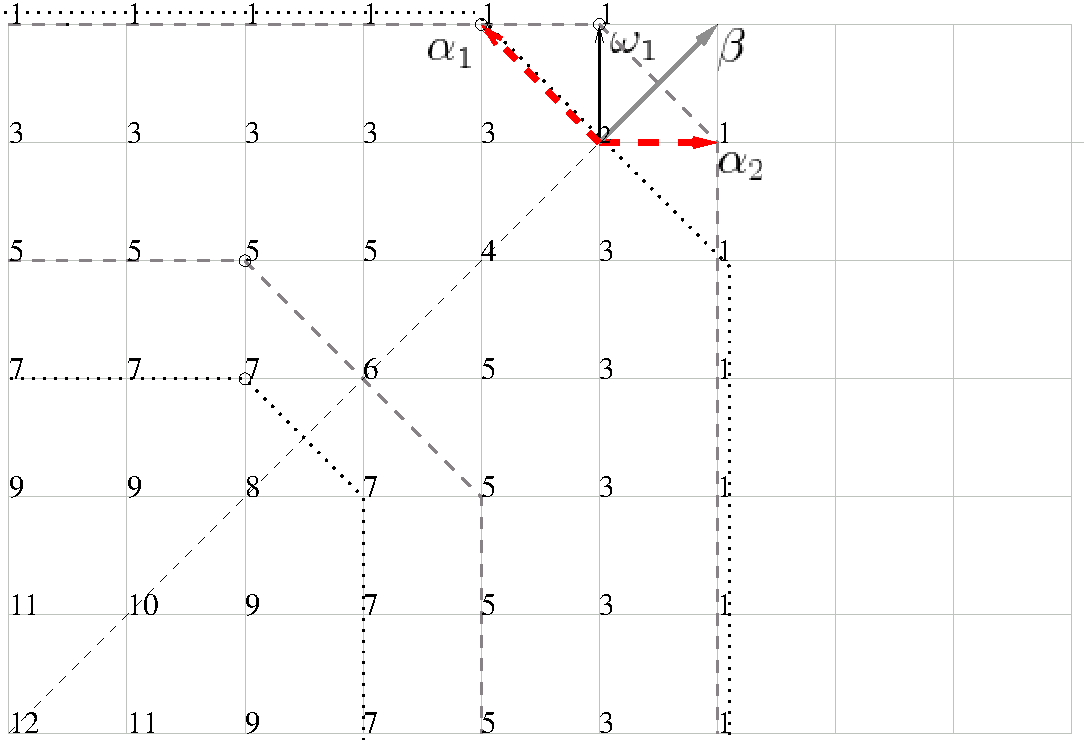
\includegraphics[width=120mm]{B2_Gen_Verma_Decomp}
  }
  \caption{Обобщенные модули Верма для регулярного вложения  $A_1$ в $B_2$. 
    Простые корни $\alpha_1, \alpha_2$ алгебры $B_2$ показаны пунктирными стрелками. Простой корень  $\beta = \alpha_1+2\alpha_2$ алгебры $A_1$ изображен серым вектором. Разложение $L^{\omega_{1}}$ представлено набором контуров входящих в него обобщенных модулей Верма. Пунктирные контуры соответствуют положительным значениям  $\epsilon(u)$, а точечные -- отрицательным. }

 \label{fig:B2_Verma_Decomp}
\end{figure}

\end{example}

\begin{remark}
Как доказано, например, в книге  \cite{humphreys2008representations} (см. утверждение 9.6), характеры обобщенных модулей Верма $M_{I}^{\mu _{\frak{a}_{\perp }}\left( u\right) }$ могут также описываться как линейные комбинации обычных модулей Верма алгебры $\frak{g}$:
\begin{equation*}
\mathrm{ch}M_{I}^{\mu _{\frak{a}_{\perp }}\left( u\right) }=\sum_{w\in W_{%
\frak{a}_{\perp }}}\epsilon \left( w\right) \mathrm{ch}M^{w\left( \mu _{%
\frak{a}_{\perp }}\left( u\right) +\rho _{\frak{a}_{\perp }}\right) -\rho _{%
\frak{a}_{\perp }}}
\end{equation*}
Подставляя это выражение в формулу (\ref{char in gen verma mod}) и используя определения  (\ref{eq:136}) и (\ref{defect-perp}), мы восстанавливаем стандартное разложение Вейля-Верма для характера:
\begin{equation*}
\mathrm{ch}\left( L^{\mu }\right) =\sum_{w\in W}\;\epsilon (u)\mathrm{ch}%
M^{w\left( \mu +\rho \right) -\rho }.
\end{equation*}
\end{remark}

\section{БГГ резольвента и ветвление}
В работе \cite{lepowsky1977generalization} показано, что для модуля старшего веса $L^{\mu }$, где $\mu \in P^{+}$, последовательность (обобщенная БГГ резольвента)
\begin{equation}
0\rightarrow M_{r}^{I}\overset{\delta _{r}}{\rightarrow }M_{r-1}^{I}\overset{%
\delta _{r-1}}{\rightarrow }\ldots \overset{\delta _{1}}{\rightarrow }%
M_{0}^{I}\overset{\varepsilon }{\rightarrow }L^{\mu }\rightarrow 0,
\label{resolution sequence}
\end{equation}
где
\begin{equation}
M_{k}^{I}=\bigoplus_{u\in U,\;\mathrm{length}\left( u\right)
=k}M_{I}^{u\left( \mu +\rho \right) -\rho },\quad M_{0}^{I}=M_{I}^{\mu }
\label{Verma elements sequence}
\end{equation}
является точной и формула (\ref{gen Weyl-Verma}%
) следует из этого разложения.

\begin{figure}[h!bt]
 \noindent\centering{
   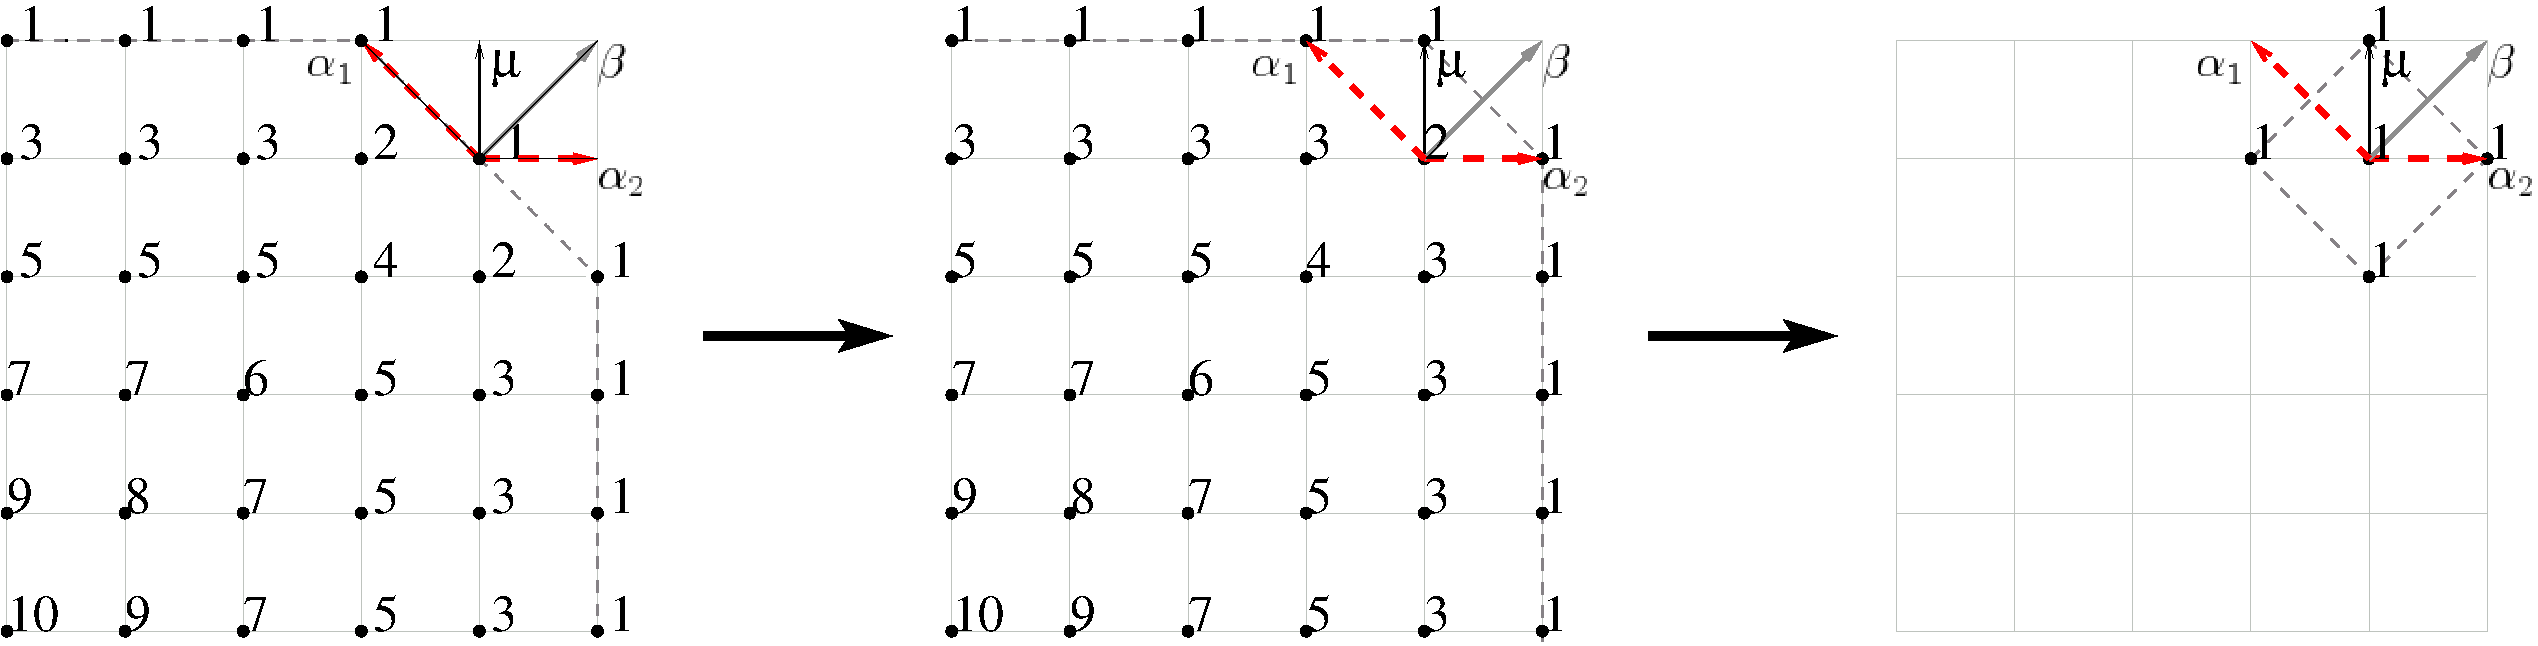
\includegraphics[width=140mm]{B2_Exact}}
 \caption{Вложение $A_1\hookrightarrow B_2$ (см. Рисунок \ref{fig:B2_Verma_Decomp}). Ортогональный партнер, подалгебра $A_1$, соответствует корню $\alpha_1$.
   Резольвента простого модуля $L^{\omega_1}$. Показана центральная часть точной последовательности
   $0 \to Im(\delta_2) \to \left( e^{\mu _{\widetilde{%
\frak{a}}}\left( e\right) }\mathrm{ch}M_{I}^{\pi _{\afb}\left[ \omega_1 \right] -%
\mathcal{D}_{\afb} }=M^{\omega_1}_{I}\right) \to
   L^{\omega_1}\to 0 $.  Здесь $\mu _{\widetilde{\frak{a}}}\left( e\right) =\pi _{\aft}\left[ \mu \right] + \mathcal{D}_{\afb}$.
   }
\end{figure}


\begin{statement}
Пусть $L^{\mu }$ --  $\frak{g}$-модуль со старшим весом $\mu \in P^{+}$, и пусть регулярная подалгебра  $\afb\hookrightarrow \frak{g}$ является ортогональным партнером редуктивной подалгебры $\frak{a}\hookrightarrow \frak{g}$. Тогда разложение (\ref{sing decomp main}) определяет как обобщенную резольвенту $L^{\mu }$ по отношению к $\afb$, так и правила ветвления $L^{\mu }$ по отношению к $\afb$, так и правила ветвления $L^{\mu }$ по отношению к $\af$ .
\end{statement}

\begin{proof}
Положим
\begin{equation*}
\mathrm{ch}M_{I}^{u\left( \mu +\rho \right) -\rho }=e^{\mu _{\widetilde{%
\frak{a}}}\left( u\right) }\mathrm{ch}M_{I}^{\mu _{\frak{a}_{\perp }}\left(
u\right) },\mathrm{ch}M_{I}^{\mu }=e^{\mu _{\widetilde{\frak{a}}}\left(
e\right) }\mathrm{ch}M_{I}^{\pi _{\frak{a}_{\perp }}\left[ \mu \right] -%
\mathcal{D}_{\frak{a}_{\perp }}},
\end{equation*}
где \ $\mu _{\widetilde{\frak{a}}}\left( u\right) ,\mu _{\frak{a}_{\perp
}}\left( u\right) $ и $\mathcal{D}_{\frak{a}_{\perp }}$ заданы как в Лемме \ref{Psi-decomp-lemma}, $%
u\in U$ определено формулой (\ref{U-def}). В результате получим элементы фильтрующей последовательности (\ref{resolution sequence}).

Рассмотрим множество $\left\{ \mu _{\frak{a}_{\perp }}\left( u\right) |u\in U\right\} $ как множество старших весов простых модулей $L_{\frak{a}%
_{\perp }}^{\mu _{\frak{a}_{\perp }}\left( u\right) }$ и вычислим размерности этих модулей. Вместе с 
$\left\{ \mu _{\widetilde{\mathfrak{a}}}\left( u\right) |u\in
U\right\} $ мы получим набор сингулярных весов
\begin{equation*}
\left\{ \epsilon (u)\;
e^{\mu _{\widetilde{\mathfrak{a}}}\left( u\right) }
\dim \left( L_{\frak{a}_{\perp }}^{\mu _{\frak{a}_{\perp
}}\left( u\right) }\right) \right\} .
\end{equation*}
Ветвление  $L_{\frak{g}\downarrow \frak{a}}^{\mu }=\bigoplus\limits_{\nu
\in P_{\frak{a}}^{+}}b_{\nu }^{\left( \mu \right) }L_{\frak{a}}^{\nu }$  определяется веером вложения  $\Gamma _{\frak{a}\rightarrow \frak{g}}$ и соотношением (\ref{recurrent-relation}), которое дает нам коэффициенты  $k_{\xi
}^{\left( \mu \right) }$, а значит определяет и  $b_{\nu }^{\left( \mu \right) }$, так как  $b_{\nu }^{\left( \mu \right) }=k_{\nu }^{\left( \mu
\right) }$ при $\nu \in \overline{C_{\frak{a}}}$ .
\end{proof}

\begin{corollary}
Пусть  $L^{\mu }$ --  $\frak{g}$-модуль со старшим весом $\mu \in P^{+}$ и  $\frak{a}\hookrightarrow \frak{g}$ -- редуктивная подалгебра $\frak{g}$. Пусть $\frak{a}_{\perp }$ -- ортогональный партнер для $\frak{a}$, -- эквивалентен  $A_{1}$, $\frak{a}_{\perp }\approx $ $A_{1}$, и $\widetilde{\frak{a}}=\frak{a}\oplus \frak{h}_{\perp }$ с $\frak{h=\frak{h}_{\frak{a}}}\oplus \frak{h}_{\frak{a}_{\perp }}\oplus \frak{h}_{\perp }$. Пусть $L_{\frak{g}\downarrow \widetilde{\frak{a}}}^{\mu }=\bigoplus\limits_{\nu \in P_{\widetilde{\frak{a}}}^{+}}b_{\nu }^{\left( \mu \right) }L_{\widetilde{\frak{a}}}^{\nu }$ -- ветвление модуля $L^{\mu }$ относительно подалгебры $\widetilde{\frak{%
a}}$. Тогда коэффициенты $b_{\nu }^{\left( \mu \right) }$ определяют обобщенную резольвенту (\ref{resolution sequence}) модуля $L^{\mu }$
по отношению к  $\frak{a}_{\perp }$.
\end{corollary}

\begin{proof}
Пусть $\alpha $ -- простой корень  $A_{1}$. Используем преобразования из группы Вейля чтобы перевести его в некоторый простой корень алгебры $\frak{g}$, например $\alpha _{1}$. Построим сингулярный элемент для модуля  $L_{\frak{g}\downarrow
\widetilde{\frak{a}}}^{\mu }$, то есть  $\Psi _{\widetilde{\frak{a}}%
}^{\left( L_{\frak{g}\downarrow \widetilde{\frak{a}}}^{\mu }\right)
}=\sum_{\nu \in P_{\widetilde{\frak{a}}}^{+},b_{\nu }^{\left( \mu \right)
}>0}b_{\nu }^{\left( \mu \right) }\Psi _{\widetilde{\frak{a}}}^{\left( \nu
\right) }$, и разложим его $\Psi _{\widetilde{\frak{a}}}^{\left( L_{\frak{%
g}\downarrow \widetilde{\frak{a}}}^{\mu }\right) }=k_{\xi }^{\left( \mu
\right) }e^{\xi }$. В нашем случае представители $u$ в рекуррентном соотношении (\ref{recurrent-relation}) определяются весом $\xi $ однозначно:
\begin{equation*}
\epsilon (u\left( \xi \right) )\;\dim \left( L_{\frak{a}_{\perp }}^{\mu _{%
\frak{a}_{\perp }}\left( u\left( \xi \right) \right) }\right) =-s\left(
\gamma _{0}\right) k_{\xi }^{\left( \mu \right) }-\sum_{\gamma \in \Gamma _{%
\widetilde{\frak{a}}\rightarrow \frak{g}}}s\left( \gamma +\gamma _{0}\right)
k_{\xi +\gamma }^{\left( \mu \right) }.
\end{equation*}
Тогда
\begin{equation*}
\dim \left( L_{\frak{a}_{\perp }}^{\mu _{\frak{a}_{\perp }}\left( u\left(
\xi \right) \right) }\right) =\left| s\left( \gamma _{0}\right) k_{\xi
}^{\left( \mu \right) }+\sum_{\gamma \in \Gamma _{\widetilde{\frak{a}}%
\rightarrow \frak{g}}}s\left( \gamma +\gamma _{0}\right) k_{\xi +\gamma
}^{\left( \mu \right) }\right|
\end{equation*}
и
\begin{equation*}
\mu _{\frak{a}_{\perp }}\left( u\left( \xi \right) \right) =\frac{1}{2}%
\left( \dim \left( L_{A_{1}}^{\mu \left( \xi \right) }\right) -1\right)
\alpha _{1}
\end{equation*}
Таким образом, множество обобщенных модулей Верма  $e^{\xi +\mathcal{D}%
_{\frak{a}_{\perp }}}\mathrm{ch}M_{I}^{\mu _{\frak{a}_{\perp }}\left(
u\left( \xi \right) \right) }$ полностью фиксировано:
\begin{equation*}
\left\{ e^{\mu _{\widetilde{\mathfrak{a}}}\left( u\right) }\mathrm{ch}%
M_{I}^{\mu _{\frak{a}_{\perp }}\left( u\right) }|u\in U\right\} .
\end{equation*}
Упорядочивая эти модули по длине $u$, мы получаем компоненты (\ref{Verma elements sequence}) резольвенты (\ref{resolution sequence}).
\end{proof}

\begin{remark}
В главе \ref{cha:affine-lie-algebras}  было показано, что метод веера вложения работает также и для специальных вложений. Надо заметить, что  разложения Вейля-Верма также могут быть получены в этом случае. Резольвенты, соответствующие специальным подалгебрам, описывают соотношения между проекциями характера начального модуля и обобщенными модулями Верма со старшими весами в подпространстве $h^*$.

Рассмотрим ситуацию, когда выбор простых корней зафиксирован какими-то внешними факторами (возникающими, например, из требований физических приложений). В этом случае ортогональный партнер не может порождаться только простыми корнями. Элементы   $\frak{u}_{I}^{+}:=\sum_{\eta \in \Delta
^{+}\setminus \Delta _{I}^{+}}\frak{g}_{\eta }$ не образуют подалгебру в  $%
\mathfrak{g}$, так как некоторые не простые корни отсутствуют в  $\Delta ^{+}\setminus
\Delta _{I}^{+}$. Важно отметить, что в этом случае формула Вейля-Верма по-прежнему существует. В ней обобщенные модули Верма соответствуют сжатиями \cite{Doebner1967Melsheimer} алгебры $%
\frak{n}^{+}$ и соотношения Вейля-Верма описывают разложение пространства представления $L^{\mu}$ в набор обобщенных модулей Верма сжатой алгебры  $U\left(\frak{n}_c^{+}\right)$. Весовые векторы образованы базисом Пуанкаре-Биркгофа-Витта алгебр $U\left(\frak{n}_c^{+}\right)$ и
$U\left( \mathfrak{a}_{\bot} \right)$. Чтобы рассмотреть такое пространство как  $%
\mathfrak{g}$-модуль мы должны выполнить деформацию \cite
{Nijenhuis1966Richardson} алгебры $\frak{n}_c^{+}$ (то есть восстановить первоначальный закон композиции). Пространство сохраняется, и после такой деформации генераторы начальной алгебры будут действовать на нем правильным образом.
\end{remark}

\section{Заключение}

\label{sec:conclusions}

Мы показали, что разложение сингулярного элемента, возникающее при редукции модулей, оказывается связано с обобщенной резольвентой Бернштейна-Гельфанда-Гельфанда. При этом веер вложения порождает параболические модули Верма. Результаты данной главы опубликованы в работах \cite{2010LyakhovskyNazarovMQFT,2011arXiv1102.1702L}.

%%
%% End of file
%%% Local Variables: 
%%% mode: latex
%%% TeX-master: "thesis"
%%% End: 


\chapter{Сплинты корневых систем и функции ветвления}
\label{cha:splints}


Сплинт корневой системы простой алгебры Ли возникает при изучении регулярных вложений редуктивных подалгебр. Сплинт можно использовать для получения правил ветвления. Мы показываем, что использование свойств сплинта  позволяет сильно упростить вычисление коэффициентов ветвления. 

Вложение  $\phi$ корневой системы $\Delta_1$ в корневую систему $\Delta$ -- это биективное отображение корней из $\Delta_{1}$ в (собственное) подмножество $\Delta$, коммутирующее с законом сложения векторов в $\Delta_{1}$ и $\Delta$.

\begin{equation*}
\phi:\Delta_1 \longrightarrow \Delta
\end{equation*}
\begin{equation*}
\phi \circ (\alpha + \beta) =\phi \circ \alpha + \phi \circ \beta,
\,\,\, \alpha,\beta \in \Delta_1
\end{equation*}

Заметим, что образ  $Im(\phi)$ не обязан обладать свойствами корневой системы за исключением правил сложения, эквивалентных правилам сложения в  $\Delta_{1}$ (для прообразов). Два вложения  $\phi_1$ и $\phi_2$  {\it расщепляют} корневую систему  $\Delta$ если она может быть представлена, как несвязное объединение образов $Im(\phi_1)$ и $Im(\phi_2)$.   
Термин {\it сплинт} (расщепление) предложил D. Richter в работе  \cite{richter2008splints}, где  были получены все сплинты для простых алгебр Ли. В работе так же упоминалось, что сплинт должен быть тесно связан с конструкцией веера вложения. Веер вложения  $\Gamma\subset \Delta$ был введен в работе  \cite{lyakhovsky1996rra} как подмножество корневой системы, описывающее рекуррентные свойства коэффициентов ветвления для максимальных вложений. Веер вложения -- это эффективный инструмент для изучения правил ветвления. Позднее в работах \cite{2010arXiv1007.0318L, ilyin812pbc} эта конструкция была обобщена на не-максимальные вложения и бесконечномерные алгебры Ли.

В данной главе мы изучаем связь между сплинтом и веером вложения для регулярных вложений редуктивных подалгебр ${\mathfrak a}$ в простую алгебру Ли $\gf$. Мы демонстрируем, что (при выполнении определенных условий, описанных в разделе \ref{sec:stems and multiplicity functions}) сплинт является естественным инструментом для изучения свойств редукции  $\gf$-модулей по отношению к подалгебре $\af\longrightarrow\gf$. Используя этот инструмент мы получаем основной результат данной главы -- однозначное соответствие между кратностями весов неприводимых модулей сплинта и коэффициентов ветвления для редуцированного модуля $L^{\mu}_{\gf\downarrow \af}$.

\section{Вложения и сплинты}

\label{sec:Injections and splints}

Рассмотрим простую алгебру Ли $\gf$ и ее  регулярную подалгебру $\af \hookrightarrow \gf$, такую, что $\af$ -- редуктивную подалгебра $\af\subset \gf$ и корневые системы согласованы $\hf_{\af}^{\ast}\subset\hf_{\gf}^{\ast}$. Пусть $\af^{\mathfrak{s}}$ -- полупростое слагаемое в $\mathfrak{a}$, то есть  $\af=\af^{\mathfrak{s}} \oplus \uf(1)\oplus \uf(1)\oplus \dots$. Мы будем считать, что $\af^{\mathfrak{s}}$ -- собственная регулярная подалгебра и что $\af$ -- максимальная подалгебра с заданной  $\af^{\mathfrak{s}}$, то есть ранг $r$ подалгебры $\af$ равен рангу $\gf$.


Пусть $L^{\mu }$ -- вполне приводимый по отношению к  $\af$ модуль алгебры $\gf$,
\[
L_{\gf\downarrow \af}^{\mu }=\bigoplus\limits_{\nu \in P_{\af%
}^{+}}b_{\nu }^{\left( \mu \right) }L_{\af}^{\nu }.
\]
\begin{equation}
\pi _{\af}ch\left( L^{\mu }\right) =\sum_{\nu \in P_{\af%
}^{+}}b_{\nu }^{(\mu )}ch\left( L_{\af}^{\nu }\right) .
\label{branching13}
\end{equation}
Для модулей, которые мы исследуем, формула Вейля для характеров $\mathrm{ch}\left(L^{\mu }\right) $ может быть записана через сингулярные элементы \cite{humphreys1997introduction}
\[
\Psi ^{\left( \mu \right) }:=\sum\limits_{w\in W}\epsilon (w)e^{w(\mu +\rho
)-\rho },
\]
а именно,
\begin{equation}
\mathrm{ch}\left( L^{\mu }\right) =\frac{\Psi ^{\left( \mu \right) }}{\Psi
^{\left( 0\right) }}=\frac{\Psi ^{\left( \mu \right) }}{R}.
\label{Weyl-Kac22}
\end{equation}
Это же верно и для подмодулей $\mathrm{ch}\left( L_{\af}^{\nu}\right) $ в уравнении (\ref{branching13})
\[
\mathrm{ch}\left( L_{\af}^{\nu }\right) =\frac{\Psi _{\af}^{\left(
\nu \right) }}{\Psi _{\af}^{\left( 0\right) }}=\frac{\Psi _{\af%
}^{\left( \nu \right) }}{R_{\af}},
\]
где
\[
\Psi _{\af}^{\left( \nu \right) }:=\sum\limits_{w\in W_{\af%
}}\epsilon (w)e^{w(\nu +\rho _{_{\af}})-\rho _{_{\af}}}.
\]

Применяя формулу (\ref{Weyl-Kac22}) к правилам ветвления (\ref{branching13}) мы получаем соотношение, связывающее сингулярные элементы $\Psi ^{\left( \mu\right) }$ и $\Psi _{\af}^{\left( \nu \right) }$ :
\begin{eqnarray}
\frac{\sum_{w \in W}\epsilon (w )e^{w (\mu +\rho )-\rho }}{\prod_{\alpha \in
\Delta ^{+}}(1-e^{-\alpha })} &=&\sum_{\nu \in P_{\af}^{+}}b_{\nu
}^{(\mu )}\frac{\sum_{w \in W_{\af}}\epsilon (w )e^{w (\nu +\rho _{%
\af})-\rho _{\af}}}{\prod_{\beta \in \Delta _{\af%
}^{+}}(1-e^{-\beta })},  \nonumber  \label{eq:132} \\
\frac{\Psi ^{\left( \mu \right) }}{R} &=&\sum_{\nu \in P_{\af%
}^{+}}b_{\nu }^{(\mu )}\frac{\Psi _{\af}^{\left( \nu \right) }}{R_{%
\af}}.  \label{singular main}
\end{eqnarray}

В работе \cite{2010arXiv1007.0318L} (см. главу \ref{cha:affine-lie-algebras}) было доказано, что коэффициенты ветвления $b_{\xi }^{\left(\mu\right)}$, отвечающие вложению $\af\hookrightarrow \gf$, удовлетворяют следующим рекуррентным соотношениям:
\begin{equation}
\begin{array}{c}
b_{\xi }^{\left( \mu \right) }=-\frac{1}{s\left( \gamma _{0}\right) }\left(
\sum_{u\in W/W_{\perp}}\epsilon (u)\;\dim \left( L_{\af_{\perp }}^{\mu _{\af%
_{\perp }}\left( u\right) }\right) \delta _{\xi -\gamma _{0},\pi _{%
\widetilde{\af}}(u(\mu +\rho )-\rho )}+\right. \\
\left. +\sum_{\gamma \in \Gamma _{\widetilde{\af}\rightarrow \gf%
}}s\left( \gamma +\gamma _{0}\right) b_{\xi +\gamma }^{\left( \mu \right)
}\right) ,
\end{array}
\label{recurrent rel}
\end{equation}
где $\afb$ -- подалгбера, задающаяся корнями  $\gf$, ортогональными ко всем корням $\af$ и $W_{\perp}$ -- подгруппа Вейля, соответствующая $\afb$,
\begin{eqnarray}
\Delta _{\af_{\perp }} &:&=\left\{ \beta \in \Delta _{\gf}|\forall
h\in \frak{h}_{\af};\beta \left( h\right) =0\right\} ,
\label{delta a ort}
\end{eqnarray}
\begin{eqnarray}
\widetilde{\af_{\perp }} :=\af_{\perp }\oplus \frak{h}_{\perp }
\qquad \widetilde{\af} :=\af\oplus \frak{h}_{\perp }
\end{eqnarray}
и $\pi$ -- оператор проекции. Если вложение максимально, то оператор проекции становится тривиальным и соотношение (\ref{recurrent rel}) упрощается:
\begin{equation}
\begin{array}{c}
b_{\xi }^{\left( \mu \right) }=-\frac{1}{s\left( \gamma _{0}\right) }\left(
\sum_{u\in W}\epsilon (u) \delta _{\xi -\gamma _{0}, u(\mu +\rho )-\rho
}+\right. \\
\left. +\sum_{\gamma \in \Gamma _{\af\rightarrow \gf}}s\left(
\gamma +\gamma _{0}\right) b_{\xi +\gamma }^{\left( \mu \right) }\right) .
\end{array}
\label{recurrent relation max}
\end{equation}
Рекурсия задается множеством  $\Gamma _{\af\rightarrow \gf}$, называющимся ``веер вложения''. Оно определяется как носитель $\left\{ \xi \right\} _{\af\rightarrow \gf}$ для коэффициентоной функции $s(\xi )$
\[
\left\{ \xi \right\} _{\af\rightarrow \gf}:=\left\{ \xi \in P_{%
\af}|s(\xi )\neq 0\right\}
\]
возникающей в разложении
\begin{equation}
\prod_{\alpha \in \Delta ^{+}\setminus \Delta _{\af}^{+}}\left( 1-e^{
-\alpha }\right) =-\sum_{\gamma \in P_{\af}}s(\gamma )e^{-\gamma };\quad
\label{product}
\end{equation}

Теперь мы приведем два определения, введенные в работе \cite{richter2008splints}

\begin{Def}
Пусть $\Delta _{0}$ и $\Delta$ -- корневые системы с соответствующими весовыми решетками $P_{0}$ и $P$. Тогда отображение $\phi $ -- ``вложение''
\begin{equation}
\phi :\left\{
\begin{array}{l}
\Delta _{0}\hookrightarrow \Delta , \\
P_{0}\hookrightarrow P,
\end{array}
\right.
\end{equation}
если \newline
\noindent (a) оно вкладывает $\Delta _{0}$ в $\Delta $, и \newline
\noindent (b) $\phi$ действует гомоморфно по отношению к группам сложения векторов в $P_{0}$ и $P$:
\[
\phi (\gamma )=\phi (\alpha )+\phi (\beta )
\]
для любой тройки $\alpha ,\beta ,\gamma \in P_{0}$, такой, что $\gamma =\alpha+\beta $.
\end{Def}

$\phi$ индуцирует вложение формальных алгебр: ${\mathcal{E}}_0\hookrightarrow \mathcal{E}$ и для образа ${\mathcal{E}}_i=\mathrm{Im}_{\phi}\left( {\mathcal{E}}_0\right)$ можно рассмотреть обратное отображение $\phi^{-1}:{\mathcal{E}}_i \longrightarrow {\mathcal{E}}_0$.

Заметим, что нужно различать два класса вложений: когда скалярное произведение (заданное формой Киллинга) в корневом пространстве $P_0$ инвариантно по отношению к  $\phi$ и когда оно не  $\phi$-инвариантно. Вложения первого класса называются ``метрическими'', второго -- ``неметрическими''. 

\begin{Def}
Корневая система $\Delta$ ``расщепляется'' на  $(\Delta _{1},\Delta _{2})$, если существует два вложения  $\phi _{1}:\Delta _{1}\hookrightarrow \Delta $ и $\phi _{2}:\Delta _{2}\hookrightarrow \Delta $, где (a) $\Delta $ -- несвязное объединение образов $\phi _{1}$ и $\phi _{2}$, и (b) ни ранг  $\Delta _{1}$, ни ранг  $\Delta _{2}$ не превосходит ранга $\Delta $.
\end{Def}

Эквивалентно, можно сказать, что  $(\Delta_1,\Delta_2)$  -- ``сплинт'' (расщепление)  $\Delta$ и мы можем обозначить его через $\Delta \approx (\Delta_1,\Delta_2)$. Каждая из компонент  $\Delta_1$ и $\Delta_2$ называется ``стеблем'' сплинта $(\Delta_1,\Delta_2)$.

Чтобы показать связь веера вложения со сплинтом рассмотрим случай, когда один из стеблей $\Delta _{1}=\Delta _{\af}$  является подсистемой корневой системы. 

Сплинт $\Delta \approx (\Delta _{1},\Delta _{2})$ называется ``инъективным'', если $\Delta _{1}=\Delta _{\af}$, -- подсистема корневой системы $\Delta $, соответствующая регулярной редуктивной подалгебре $\af\hookrightarrow \gf$. 

В случае инъективного сплинта второй стебель $\Delta _{\sfr}:=\Delta_{2}=\Delta \setminus \Delta _{\af}$ может быть переписан как произведение (\ref{product}) и определяет веер вложения  $\Gamma _{\af\hookrightarrow \gf}$. Обозначим через $\Delta_{\mathfrak{s}0}$ кообраз второго вложения $\phi:\Delta_{\mathfrak{s}0}\to \Delta_{\gf}$. Верна следующая гипотеза.

\begin{Cnj}
Каждый инъективный сплинт $\Delta \approx (\Delta _{\af},\Delta _{\sfr})$ определяет веер вложения с носителем $\left\{ \xi \right\} _{\af\rightarrow \gf}$, задающимся произведением
\begin{equation}
\prod_{\beta \in \Delta _{\sfr}^{+}}\left( 1-e^{-\beta }\right)
=-\sum_{\gamma \in P}s(\gamma )e^{-\gamma }\quad   \label{splint product}
\end{equation}
\end{Cnj}

В случае инъективного сплинты мы можем сказать, что подалгебра $\af\hookrightarrow \gf$ расщепляется $\Delta$ (и назовем $\af$ ``расщепляющей подалгеброй'' алгебры $\gf$).  Сплинты были классифицированы в работе \cite{richter2008splints}  (см. Приложение в конце главы) и первые три класса сплинтов в этой классификации инъективны. 

\section{Как стебли определяют функции кратности}

\label{sec:stems and multiplicity functions}

В этом разделе мы рассмотрим свойства инъективных сплинтов $\Delta \approx (\Delta _{\af},\Delta _{\sfr})$. Мы покажем, что в этом случае вычисление коэффициентов ветвления для расщепляющего вложения $\af\hookrightarrow\gf$ эквивалентно нахождению кратностей весов неприводимого $\sfr$-модуля $L_{\sfr}^{\nu }$ с определенным старшим весом $\nu $. Заметим, что алгебра $\sfr$ не обязательно должна быть подалгеброй $\gf$.

Вернемся к соотношению  (\ref{singular main}) и домножим обе стороны на  $R_{\af}$:
\begin{equation}
\frac{1}{\prod_{\beta \in \Delta _{\sfr}^{+}}(1-e^{-\beta })}\Psi _{\gf}^{\left( \mu \right) }=\sum_{\nu \in P_{\af}^{+}}b_{\nu}^{(\mu )}\Psi _{\af}^{\left( \nu \right) }.
\label{singular main-2}
\end{equation}
Здесь первый множитель в левой части -- это формальный элемент, обратный к вееру $\Gamma _{\af\rightarrow \gf}$. Рассмотрим модуль старшего веса $L_{\sfr}^{\nu }$. Вложение $\phi :\Delta _{\sfr\,0}\longrightarrow \Delta_{\gf}$ переводит сингулярный элемент  $\Psi _{\sfr}^{\left( \nu\right) }$ в $\Psi _{\gf}^{\left( \mu \right) }$. Применяя обратный морфизм $\phi ^{-1}$ к произведению $\left( \prod_{\beta \in \Delta_{\sfr}^{+}}(1-e^{-\beta })\right) ^{-1}\phi \left( \Psi _{\sfr}^{\left( \nu \right) }\right) $, мы получаем характер модуля $L_{\sfr}^{\nu }$,

\begin{equation}
\phi ^{-1}\left( \frac{1}{\prod_{\beta \in \Delta _{\sfr%
}^{+}}(1-e^{-\beta })}\phi \left( \Psi _{\sfr}^{\left( \nu \right)
}\right) \right) =\frac{1}{\prod_{\beta \in \Delta _{\sfr0
}^{+}}(1-e^{-\beta })}\Psi _{\sfr}^{\left( \nu \right) }=\mathrm{ch}%
\left( L_{\sfr}^{\nu }\right) .  \label{inverse for stem}
\end{equation}
Наша задача состоит в том, чтобы доказать, что сингулярный элемент $\Psi _{\gf}^{\left(\mu\right) }$ содержит элемент $\Psi _{\sfr}^{\left( \xi \right) }$ для модуля $L_{\sfr}^{\xi }$, однозначно определяемого модулем $L_{\gf}^{\mu }$ и что коэффициенты ветвления $b_{\nu }^{(\mu )}$ в правой части равенства (\ref{singular main-2}) совпадают с кратностями $m_{\zeta }^{\left( \xi\right) }$ соответствующих весов в $\mathcal{N}_{\sfr}^{\xi }$ .

Для неприводимого модуля старшего веса $L_{\gf}^{\mu }$ сингулярный элемент $\Psi _{\gf}^{\left( \mu \right) }$ -- это элемент $\mathcal{E}$, соответствующий сдвинутой орбите группы веса $\left( \mu +\rho\right) \in P^{+}$, со знаковой функцией $\epsilon \left( w\right) $. Удобно использовать также не сдвинутые сингулярные элементы
\begin{equation}
\Phi ^{\left( \mu \right) }:=\Psi ^{\left( \mu \right) }e^{\rho }.
\label{definition Phi}
\end{equation}
В этих обозначениях соотношение (\ref{singular main-2}) имеет вид
\begin{equation}
\frac{e^{\rho _{\gf}-\rho _{\af}}}{\prod_{\beta \in \Delta _{\frak{%
s}}^{+}}(1-e^{-\beta })}\Phi _{\gf}^{\left( \mu \right) }=\sum_{\nu \in
P_{\af}^{+}}b_{\nu }^{(\mu )}\Phi _{\af}^{\left( \nu \right) }.
\label{singular main-3}
\end{equation}
Орбита, связанная с  $\Phi _{\gf}^{\left( \mu \right) }$, полностью определяется набором ребер $\left\{ \lambda _{i}\right\} _{i=1,\dots ,r}$ построенным из конца вектора старшего веса $\mu +\rho $. Для $\mu=\sum m_{i}\omega _{i}$ эти ребра равны
\begin{equation}
\lambda _{i}=-\left( m_{i}+1\right) \alpha _{i},\quad i=1,\dots ,r.
\label{edge}
\end{equation}
Каждая формальная экспонента $e^{\mu +\rho +\lambda _{i}}$ in $\Phi _{\gf}^{\left( \mu \right) }$ снабжена знаковым коэффициентом  $\epsilon =(-)$. Можно определить $\Phi_{\gf}^{\left( \mu \right) }$ следующим свойством. Рассмотрим любую пару ребер $\lambda _{i},\lambda _{j}$ и соответствующие веса $\mu +\rho $, $\mu +\rho +\lambda _{i}$ и $\mu +\rho +\lambda _{j}$. 
Применим отражение $s_{\alpha _{i}}$ (or $s_{\alpha _{j}}$),
\begin{equation}
s_{\alpha _{i}}\circ \left\{
\begin{array}{l}
\left( \mu +\rho \right)  \\
\left( \mu +\rho +\lambda _{i}\right)  \\
\left( \mu +\rho +\lambda _{j}\right)
\end{array}
\right. =\left\{
\begin{array}{l}
\left( \mu +\rho +\lambda _{i}\right)  \\
\left( \mu +\rho \right)  \\
\left( \mu +\rho +\lambda _{i}-(m_{j}+1)s_{\alpha _{i}}\circ \alpha
_{j}\right)
\end{array}
\right.   \label{reflected triple}
\end{equation}

\begin{Prop}
Ребро  $\lambda _{i,j}$ сингулярного элемента $\Phi _{\gf}^{\left( \mu \right) }$, начинающееся в весе $\left( \mu +\rho +\lambda _{i}\right) $ и направленное вдоль корня $-s_{\alpha _{i}}\circ \alpha _{j}$ имеет такую же длину, выраженную в длинах корня $(s_{\alpha_{i}}\circ \alpha _{j})$, как и $\lambda _{j}$ в длинах $\alpha _{j}$. (Это же верно для ребра $\lambda _{j,i}$, его длина в единицах $(s_{\alpha _{j}}\circ\alpha _{i})$ равна длине $\lambda _{i}$ в единицах $\alpha _{i}$.)
\label{diagram property}
\end{Prop}

В $\Phi _{\gf}^{\left( \mu \right) }$ элементы $e^{\left( \mu+\rho +\lambda_{i}-(m_{j}+1)s_{\alpha _{i}}\circ \alpha _{j}\right) }$ и $e^{\left( \mu +\rho +\lambda _{j}-(m_{i}+1)s_{\alpha_{j}}\circ \alpha_{i}\right) }$ имеют знаковый коэффициент  $\epsilon =(+)$.

Вспомним, что только три типа сплинтов инъективны и имеют естественную связь с ветвлениями. Ниже мы приводим часть таблицы сплинтов из работы \cite{richter2008splints}, соответствующую инъективным сплинтам:
\[
\begin{array}{cc||c|c}
\hbox{тип} & \hspace{0.25in}\Delta \hspace{0.25in} & \hspace{0.25in}\Delta
_{\af}\hspace{0.25in} & \hspace{0.25in}\Delta _{\sfr}\hspace{0.25in}
\\ \hline\hline
\hbox{(i)} & G_{2} & A_{2} & A_{2} \\
& F_{4} & D_{4} & D_{4} \\ \hline
\hbox{(ii)} & B_{r}(r\geq 2) & D_{r} & \oplus ^{r}A_{1} \\
& C_{r}(r\geq 3) & D_{r} & \oplus ^{r}A_{1} \\ \hline
\hbox{(iii)} & A_{r}(r\geq 2) & A_{r-1}\oplus u\left( 1\right)  & \oplus
^{r}A_{1} \\
& B_{2} & A_{1}\oplus u\left( 1\right)  & A_{2}
\end{array}
\]

Каждая строка в таблице соответствует сплинту  $(\Delta _{\af},\Delta _{\sfr})$  корневой системы $\Delta $. В случае первых двух типов и  $\Delta _{\af}$, и $\Delta _{\sfr}$ вложены метрически. Стебли для первого типа эквивалентны, а для второго -- нет. В случае третьего типа сплинтов только корневая система $\Delta _{\af}$ вложена метрически. Слагаемые $u\left( 1\right) $ добавлены, чтобы совпадали ранги $r_{\af}=r$. Такая добавка не меняет основных свойств ветвления, но позволяет использовать кратности весов $\sfr$-модулей без последующей проекции весов.

Сплинт индуцирует разложение множества $S=S_{\frak{c}}\cup S_{\frak{d}}$, где $S_{\frak{c}}=S\cap S_{\af}$ и $S_{\frak{d}}=S\cap S_{\sfr}$.  Легко проверить, что для любого инъективного сплинта подмножество  $S_{\frak{d}}$ не пусто. Следовательно, в множестве $\left\{ \lambda
_{i}\right\} _{i=1,\dots ,r}$ всегда найдется простые корни $\beta_{k}\in \Delta _{\sfr}$ и орбита, соответствующая $\Phi _{\gf}^{\left( \mu \right) }$ будет содержать ребра
\begin{equation}
\lambda _{k}=-\left( m_{k}+1\right) \beta _{k}  \label{beta edge},
\end{equation}
построенные из веса  $\mu +\rho $.  Так как $\Delta _{\af}$ -- корневая система и для любой пары простых корней из $S_{\frak{c}}$ выполнено свойство \ref{diagram property}, элемент  $\Phi _{\gf}^{\left( \mu \right) }$ является сингулярным элементом для набора  $\af$-модулей. Рассмотрим корень $\beta _{l}\in \Delta _{\sfr}$, кообраз которого в  $\Delta _{\sfr0}$  простой. В разделе \ref{sec:appendix} мы показываем, что для каждого такого $\beta _{l}$ существует корень  $\alpha _{l}\in S_{\frak{c}}$, такой, что $\beta _{l}=\alpha _{l}+\beta _{k}$. Легко видеть, что в этом случае соответствующее ребро пересекает гиперплоскость, ограничивающую главную камеру Вейля$ \bar{C_{\af}}$ и ортогональную к корню $\alpha _{l}$,
\begin{equation}
s_{\alpha _{l}}\left( \mu +\rho -p\beta _{l}\right) =s_{\alpha _{l}}\left(
\mu +\rho \right) -ps_{\alpha _{l}}\beta _{l}=\mu +\rho -p\beta _{l},
\label{intersection}
\end{equation}
\begin{equation}
\mu +\rho -s_{\alpha _{l}}\left( \mu +\rho \right) =\left( m_{l}+1\right)
\alpha _{l}=\left( m_{l}+1\right) \beta _{l}-\left( m_{l}+1\right) \beta
_{k}=p\beta _{l}-ps_{\alpha _{l}}\beta _{l}.  
\label{intersection-2}
\end{equation}
Следовательно,  $p=\left( m_{l}+1\right) $ и  $s_{\alpha _{l}}\beta_{l}=\beta _{k}$. Теперь применим оператор $s_{\beta _{k}}$ и заметим, что ребро, построенное вдоль корня $s_{\beta _{k}}\alpha _{l}$ из веса $s_{\beta _{k}}(\mu +\rho )$ тоже равно $-ps_{\beta _{k}}\alpha _{l}$. Значит, для тройки корней  $\beta _{k},\beta _{l}$ и $s_{\beta _{k}}\alpha _{l}$ in $\Delta _{\sfr}$ ребра $\lambda_{k}=-\left( m_{k}+1\right) \beta _{k}$, $\lambda _{l}=-\left(m_{l}+1\right) \beta _{l}$ и $\lambda _{kl}=-\left( m_{l}+1\right)s_{\beta _{k}}\alpha _{l}$ удовлетворяют свойству \ref{diagram property}.
Эту процедуру можно продолжить далее в двумерном подпространстве, заданном корнями $\beta _{k}$ и $\beta _{l}$ и показать, что множество формальных экспонент, снабженных соответствующими знаковыми множителями, составляет кообраз сингулярного элемента модуля подалгебры в  $\frak{
s}$ (ранг этой подалгебры $r=2$).

Аналогичное рассуждение  можно провести для любого положительного корня $\beta _{l}\in \Delta $, являющегося простым в $\Delta _{\sfr0}$ и, соответственно, для любой подалгебры ранга $r=2$ в $\sfr$. То есть чтобы ``найти'' сингулярный элемент $\sfr$-модуля в $\Phi_{\gf}^{\left( \mu \right) }$ необходимо сгруппировать с ним дополнительные формальные элементы  $\left\{ -e^{\mu +\rho-\left( m_{l}+1\right) \beta _{l}}|\beta _{l}\in S_{\frak{c}}\right\}.$ Эта процедура определяет начальные ребра диаграммы $\phi ^{-1}\left( \Phi _{\sfr}^{\widetilde{\mu }}\right) $. Как следует из процедуры восстановления, старший вес $\widetilde{\mu }$ полностью определяется весом $\mu $, эти веса имеют следующие индексы Дынкина:
\begin{equation}
\mu =\sum m_{k}\omega _{k}\qquad \Longrightarrow \quad \widetilde{\mu }=\sum
m_{k}\widetilde{\omega }_{k} . \label{new h weight}
\end{equation}
Следующим шагом построим полную  $W_{\sfr}$-орбиту элемента $\Phi _{\sfr}^{\left( \widetilde{\mu }\right) }$  в $P_{\sfr}$. Легко видеть, что его кообраз принадлежит  $\bar{C_{\af}}$ и что множество $\phi^{-1}\left( \Phi _{\sfr}^{\widetilde{\mu }}\right) \setminus \Phi _{\gf}^{\left( \mu \right) }|_{\bar{C_{\af}}}$ соответствует весам, принадлежащим границе$\bar{C_{\af}}$ (включая подмножество $\left\{ -e^{\mu +\rho -\left( m_{l}+1\right) \beta _{l}}|\beta _{l}\in S_{\frak{c}}\right\} $). То есть мы построили все формальные элементы с соответствующими знаковыми множителями, которые после сложения с  $\Phi _{\gf}^{\left( \mu \right) }|_{\bar{C_{\af}}}$ образуют диаграмму $\phi^{-1}\left( \Phi _{\sfr}^{\widetilde{\mu }}\right) $ в $\bar{C_{\af}}$.

Теперь вернемся к равенству (\ref{singular main-3}). Можно добавить к $\Phi _{\gf}^{\left( \mu \right) }$ пары формальных элементов, построенные выше, с противоположными знаками: $\epsilon \left( w\right)|_{w\in W_{\sfr}}$ and $-\epsilon \left( w\right) |_{w\in W_{\sfr}}$. 
Припишем знаки $\epsilon \left( w\right) |_{w\in W_{\sfr}}$ элементам, веса которых попадут в главную камеру $\bar{C_{\af}}$. К соседним камерам $\bar{C_{\af}^{(l)}}$ относятся те же элементы, но  с противоположным знаком  (Эти камеры связаны с главной простыми отражениями $s_{\alpha _{l}}$, так что противоположные знаки $-\epsilon \left( w\right) |_{w\in W_{\sfr}}$ здесь естественны). Можно повторить эту процедуру и получить дополнительные сингулярные веса в любой камере Вейля $\bar{C_{\af}^{(m)}}$, причем эти веса будут иметь знаки, противоположные знакам в соседних камерах. То есть не меняя элемент $\Phi _{\gf}^{\left( \mu \right) }$ его можно представить в виде суммы
\begin{equation}
\Phi _{\gf}^{\left( \mu \right) }=\sum_{w\in W_{\af}}w\circ \left(
e^{\rho _{\af}}\Psi ^{\widetilde{\mu }+\rho _{\sfr}}\right)
\label{singular final}
\end{equation}
где вес $\widetilde{\mu }=\sum m_{k}\omega _{\sfr}^{k}$ был введен выше. Разложение (\ref{singular final}) позволяет применить множитель $\left( \prod_{\beta \in \Delta _{\sfr}^{+}}(1-e^{-\beta })\right) ^{-1}$ к каждому слагаемому сингулярного элемента  $\Phi _{\gf}^{\left( \mu \right)}$ по отдельности, так как множества весов различных слагаемых Вейля не пересекаются. Воспользовавшись изоморфизмом  $\phi $ мы видим, что в главной камере Вейля  $\bar{C_{\af}}$ множество весов, порожденное действием $\left( \prod_{\beta\in \Delta _{\sfr}^{+}}(1-e^{-\beta })\right)^{-1}$ изоморфно весовой диаграмме  $\mathcal{N}_{\sfr}^{\widetilde{\mu }}$  модуля  $L_{\sfr}^{\widetilde{\mu }}$ алгебры $\sfr$. Теперь можно ограничить равенство (\ref{singular main-3}) на главную камеру Вейля $\bar{C_{\af}}$ и получить основной результат этого раздела:
\begin{Prop}
\begin{equation}
\frac{e^{\rho _{\gf}}}{\prod_{\beta \in \Delta _{\sfr%
}^{+}}(1-e^{-\beta })}\left( \Psi ^{\widetilde{\mu }+\rho _{\sfr%
}}\right) =\sum_{\widetilde{\nu }\in \mathcal{N}_{\sfr}^{\widetilde{\mu }%
}}M_{\left( \sfr\right) \widetilde{\nu }}^{\widetilde{\mu }}e^{\left(
\mu -\phi \left( \widetilde{\mu }-\widetilde{\nu }\right) \right)
}=\sum_{\nu \in P_{\af}^{++}}b_{\nu }^{(\mu )}e^{\nu }.
\label{singular main-4}
\end{equation}
Любой вес с ненулевой кратностью, входящий в правую часть равенства, равен одному из старших весов в разложении. Кратность $M_{\left( \sfr
\right) \widetilde{\nu }}^{\widetilde{\mu }}$ веса  $\widetilde{\nu}\in \mathcal{N}_{\sfr}^{\widetilde{\mu }}$ определяет коэффициент ветвления  $b_{\nu }^{(\mu )}$ для старшего веса $\nu =\left( \mu-\phi \left( \widetilde{\mu }-\widetilde{\nu }\right) \right) $:
\[
b_{\left( \mu -\phi \left( \widetilde{\mu }-\widetilde{\nu }\right) \right)
}^{(\mu )}=M_{\left( \sfr\right) \widetilde{\nu }}^{\widetilde{\mu }}.
\]
\end{Prop}

\section{Примеры}
\label{sec:examples}
\begin{example}
\label{example-1}
Рассмотрим алгебру Ли $A_{2} =\bf{sl}(3)$ и ветвление ее неприводимого модуля $L^{[3,2]}_{A_{2}}$ по отношению к редуктивной подалгебре $A_{1}\oplus u(1)$. Корневая система  $\Delta _{\af}= \Delta_{A_{1}\oplus u(1)}$ содержит простой корень $\alpha_1=e_1-e_2$ алгебры $A_{2}$. Сингулярный элемент $\Psi^{[3,2]}_{\af}$ раскладывается в сумму образов сингулярных элементов  модулей алгебры $A_{1}\oplus A_{1}$. Коэффициенты ветвления $b_{\nu }^{[ 3,2 ] }$ совпадают с кратностями весов модуля $L^{[3,2]}_{A_{1}\oplus A_{1}}$ (см. Рисунок. \ref{fig:a2_splint}).

  \begin{figure}[h!bt]
  \noindent\centering{
   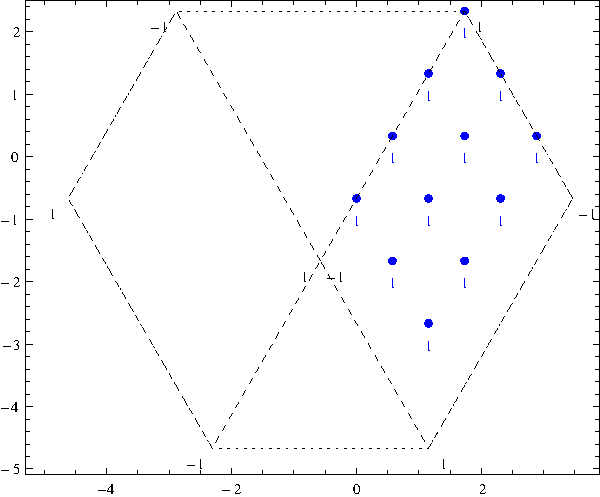
\includegraphics[width=80mm]{a2-a1}
  }
  \caption{Орбита группы Вейля (точечный контур), соответствующая сингулярному элементу $L^{[3,2]}_{A_{2}}$ и ее разложение в сумму образов сингулряных элементов модулей  $L^{[3,2]}_{A_{1}\oplus A_{1}}$ (пунктирные контуры). Кратности весов модуля $L^{[3,2]}_{A_{1}\oplus A_{1}}$ совпадают  с коэффициентами ветвления для редукции $L^{[3,2]}_{A_{2}\downarrow A_{1}\oplus u(1)}$.}

 \label{fig:a2_splint}
\end{figure}
\end{example}
\begin{example}
\label{example-2}
 Рассмотрим алгебру Ли $B_{2}= \bf{so}(5)$ и редукцию ее неприводимого модуля  $L^{[3,2]}$ на модули редуктивной подалгебры  $A_{1}\oplus u(1)$ с корневой системой, натянутой на первый простой корень $\alpha_1=e_1-e_2$ алгебры $B_{2}$. Сингулярный элемент $\Psi^{[3,2]}_{B_{2}}$ раскладывается в сумму образов сингулярных элементов модулей $A_{2}$ и коэффициенты ветвления совпадают с кратностями весов в модуле $A_{2}$ (см. Рисунок \ref{fig:b2_splint}).

  \begin{figure}[h!bt]
  \hspace*{-1.2cm}

   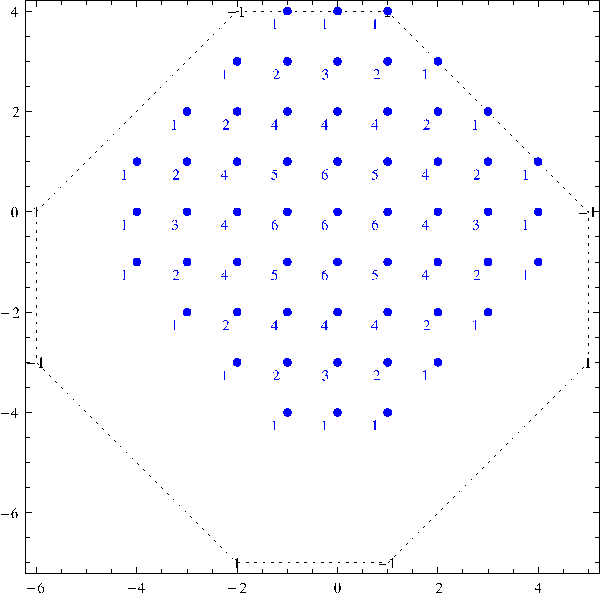
\includegraphics[width=65mm]{b2}
   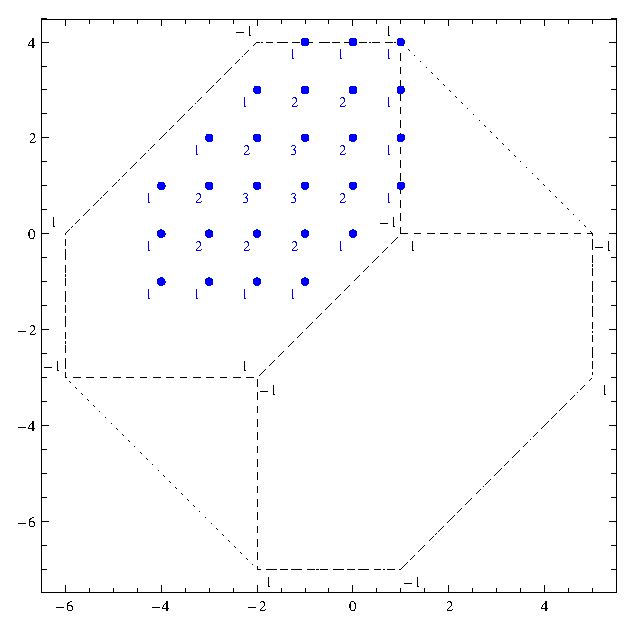
\includegraphics[width=65mm]{b2-a2-a1}
  \caption{Веса модуля  $L^{[3,2]}$ алгебры  $B_{2}$ показаны точками на левом рисунке (кратности подписаны). Контур сингулярного элемента показан коротким пунктиром. На правом рисунке представлено разложение сингулярного элемента $\Psi_{B_{2}}(L^{[3,2]}_{B_{2}})$ в сумму образов сингулярных элементов $\Psi_{A_{2}}(L^{[3,2]})$ (длинный пунктир). Кратности весов модуля $L^{[3,2]}_{A_{2}}$ совпадают с коэффициентами ветвления для редукции $L^{[3,2]}_{B_{2}\downarrow A_{1}\oplus u(1)}$.}

 \label{fig:b2_splint}
\end{figure}
\end{example}

\vspace{10mm}
\begin{example}
  Алгебра Ли  $G_{2}$ содержит регулярную подалгебры  $A_{2}$ с корневой системой $\Delta_{\af}=\Delta_{A_{2}}$, содержащей длинные корни $G_{2}$. Рассмотрим ветвление неприводимого модуля $L_{G_{2}}^{(3,2)}$ на модули подалгебры $A_{2}$. Сингулярный элемент $\Psi_{G_{2}}(L^{[3,2]})$ раскладывается в сумму образов сингулярных элементов  $\Psi_{A_{2}}(L^{[3,2]})$ и коэффициенты ветвления совпадают с кратностями весов модуля $L^{[3,2]}_{A_{2}}$ (см. Рисунок \ref{fig:g2_splint}).


  \begin{figure}[h!bt]
  \noindent\centering{
   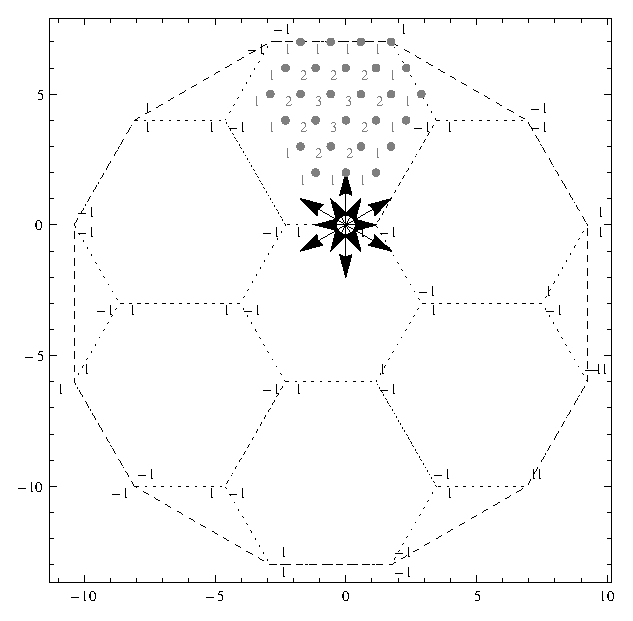
\includegraphics[width=120mm]{g2}
  }

  \caption{Орбита группы Вейля  (короткий пунктир) для сингулярного элемента  $\Psi_{G_{2}}(L^{[3,2]})$ и его разложение в сумму образов сингулярных элементов модулей алгебры $A_{2}$ (длинный пунктир). Кратности весов модуля $L^{[3,2]}_{A_{2}}$ совпадают с коэффициентами ветвления для редукции $L^{[3,2]}_{G_{2}\downarrow A_{2}}$.}


 \label{fig:g2_splint}
\end{figure}

\end{example}

\section{Сплинты и соотношения для аффинных алгебр Ли}
\label{sec:splints-affine}

Splint of root system of simple Lie algebra appears naturally in
the study of (regular) embeddings of reductive subalgebras. It can
be used to derive branching rules. Application of
splint properties drastically simplifies calculations of
branching coefficients. We study affine extension of splint root system of simple Lie algebra and obtain relations on theta and branching functions.

The term {\it splint} was introduced by D. Richter in \cite{richter2008splints} where the
classification of splints for simple Lie algebras was obtained. The fan $\Gamma \subset \Delta$ was
introduced in \cite{lyakhovsky1996rra} as a subset of root system describing recurrent properties of
branching coefficients for maximal embeddings. Injection fan is an efficient tool to study branching
rules. Later this construction was generalized to non-maximal embeddings and affine Lie algebras in
\cite{2010arXiv1007.0318L, ilyin812pbc}. In paper \cite{2011arXiv1111.6787L} we have shown that the
existence of a splint for a root system of a simple Lie algebra leads to simplifications in
reduction procedures of a Lie algebra module to modules of a subalgebra. This effect is based on the
injection fan and singular element properties of Lie algebra modules.

In the present note we discuss possible applications of splint in
a root system of simple Lie algebra related to representation
theory of affine Lie algebras. We discuss the structure of
injection fan for affine Lie algebras and show that it admits a
decomposition similar to that used in \cite{2011arXiv1111.6787L}
for simple Lie algebras. Such a decomposition leads to equations
for theta-functions. We study graded branching of affine Lie
algebra modules reduced to a finite-dimensional subalgebra and
discuss consequences of splint in this case.

\subsection{Splints and affine Lie algebras}
\label{sec:definitions}

Consider simple Lie algebra $\gf$ with a root system $\Delta$. Let
$\af_{1}\subset \gf$ be its reductive subalgebra of the same rank, such that
$\Delta_{\af}\equiv\Delta_{1}\subset\Delta$ and $Q_{\af}\subset Q$, where $Q$ is the root lattice. Irreducible highest-weight modules of
$\gf$ and $\af$ are denoted by $L^{\mu}$ and $L^{\nu}_{\af}$
correspondingly. Weyl character formula for irreducible modules is
$\mathrm{ch}L^{\mu}=\frac{\Psi^{(\mu)}}{\prod_{\alpha\in\Delta}(1-e^{-\alpha})}$,
where $\Psi^{(\mu)}=\sum_{w\in W}\epsilon(w) e^{w(\mu+\rho)-\rho}$
is a singular element of the module and $W$ -- the Weyl group of
$\gf$. Formal character of irreducible module admits a
decomposition
\begin{equation}
  \label{eq:133}
  \mathrm{ch} L^{\mu}=\sum_{\nu\in P_{\af}} b^{\mu}_{\nu} \mathrm{ch} L^{\nu}_{\af},
\end{equation}
where $P$, $P_{\af}$ are weight lattices of $\gf$ and $\af$. We
want to study affine extension of this situation:
$\gf\subset\gfh,\; \af\subset\afh$, $\afh\subset\gfh$,
$\hat{\Delta}\subset\hat{\Delta}$ and
$\mathrm{ch}L^{\hat{\mu}}_{\gfh}=\sum_{\hat{\nu}}
b^{\hat{\mu}}_{\hat{\nu}} \mathrm{ch} L^{\hat{\nu}}_{\afh}$. For
weights of an affine Lie algebra $\gfh$ we have
$\hat{\mu}=(\mu,k,n)$, where $\mu$ is a weight of $\gf$, $k$ --
the level of the module and $n$ -- the grade of the weight
$\hat{\mu}$

\begin{Def}
  Embedding $\phi$ of a root system $\Delta_1$ into a root system $\Delta$ is a bijective map of
  roots of $\Delta_{1}$ to a (proper) subset of $\Delta$ that commutes with vector composition law
  in $\Delta_{1}$ and $\Delta$.
\begin{equation*}
\phi:\Delta_1 \longrightarrow \Delta, \quad \phi \circ (\alpha + \beta) =\phi \circ \alpha + \phi \circ \beta,\,\,\, \alpha,\beta \in \Delta_1
\end{equation*}
\end{Def}

Note that the image $Im(\phi)$ must not inherit the root system properties except the addition rules
equivalent to the addition rules in $\Delta_{1}$ (for pre-images). Two embeddings $\phi_1$ and
$\phi_2$ can splinter $\Delta$ when the latter can be presented as a disjoint union of images
$Im(\phi_1)$ and $Im(\phi_2)$.

$\phi$ induces an injection of formal algebras $:{\mathcal{E}}_0
\hookrightarrow \mathcal{E}$ and for the image ${\mathcal{E}}%
_i=Im_{\phi}\left( {\mathcal{E}}_0\right)$ one can consider its inverse $%
\phi^{-1}:{\mathcal{E}}_i \longrightarrow {\mathcal{E}}_0$.

\begin{Def}
  A root system $\Delta $ ''splinters'' as $(\Delta _{1},\Delta _{2})$ if there are two embeddings
  $\phi _{1}:\Delta _{1}\hookrightarrow \Delta $ and $%
  \phi _{2}:\Delta _{2}\hookrightarrow \Delta $ where (a) $\Delta $ is the disjoint union of the
  images of $\phi _{1}$ and $\phi _{2}$ and (b) neither the rank of $\Delta _{1}$ nor the rank of
  $\Delta _{2}$ exceeds the rank of $%
  \Delta $.
\end{Def}

It is equivalent to say that $(\Delta_1,\Delta_2)$ is a "splint'' of $\Delta$ and we shall denote
this by $\Delta \approx (\Delta_1,\Delta_2)$. Each component $\Delta_1$ and $\Delta_2$ is a "stem''
of the splint.

We consider the case when one of the stems $\Delta _{1}=\Delta _{\frak{a}}$ is a root subsystem. As shown in paper \cite{2011arXiv1111.6787L} the second stem $\Delta _{\frak{s}}:=\Delta
_{2}=\Delta \setminus \Delta _{\frak{a}}$ can be translated into a product
$\prod_{\beta \in \Delta _{\frak{s}}^{+}}\left( 1-e^{-\beta }\right)=-\sum_{\gamma \in P}s(\gamma )e^{-\gamma }\quad   \label{splint product}$
and it defines an injection fan $\Gamma _{\frak{a}%
\hookrightarrow \frak{g}}$ \cite{lyakhovsky1996rra,ilyin812pbc,2010arXiv1007.0318L}.

Since the singular element of $L^{\mu}$ can be
written as $\Psi _{\frak{g}}^{\left( \mu \right) }=e^{-\rho }
\sum_{w\in W_{\frak{a}}}\epsilon \left( w \right) w\circ \left(
e^{\rho _{\frak{a}}}\Psi ^{\widetilde{\mu }+\rho
_{\frak{s}}}\right)$  for branching coefficients we get the
identity \cite{2011arXiv1111.6787L}:
\begin{equation}
  \label{eq:146}
b_{\left( \mu -\phi \left( \widetilde{\mu }-\widetilde{\nu }\right) \right)
}^{(\mu )}=M_{\left( \frak{s}\right) \widetilde{\nu }}^{\widetilde{\mu }}  
\end{equation}
Here the highest weight $\widetilde{\mu }$ is totally defined by the weight $\mu $, they have the
same Dynkin numbers: $\mu =\sum m_{k}\omega _{k}\qquad \Longrightarrow \quad \widetilde{\mu }=\sum
m_{k}\omega_{(\sfr) k} . \label{new h weight}$ So branching coefficients coincide with weight
multiplicities of $\sfr$-modules.

Now we consider affine extension of this setup, $\afh\subset\gfh$. Since $\mathrm{rank}\gf\leq
\mathrm{rank} \af+\mathrm{rank}\sfr$ for Weyl denominators we get
 \[
\prod_{\alpha\in\hat{\Delta}^{+}_{1}}(1-e^{-\alpha})^{\mathrm{mult}(\alpha)}\prod_{\beta\in\hat{\Delta}^{+}_{2}}(1-e^{\phi\circ \beta})^{\mathrm{mult}(\beta)}=\prod_{\gamma\in\hat{\Delta}^{+}}(1-e^{-\gamma})^{\mathrm{mult}(\gamma)}\prod_{n=0}^{\infty}(1-e^{-n\delta})^{\mathrm{rank}\af+\mathrm{rank}\sfr-\mathrm{rank}\gf}
\]

Using a specialization
\cite{kac1988modular,kac1984infinite,kac1990idl} and the
definition of Dedekind eta-function
$\eta(\tau)=q^{1/24}\prod_{n=1}^{\infty}(1-q^{n})$, where
$q=e^{2\pi i \tau}$ we can rewrite this identity as the relation
imposed on theta-functions $\Theta^{(\gfh)}_{\widehat{\lambda}=(\lambda,k,0)}(\tau,z)=\sum_{\xi\in Q_{\gf}+\frac{\lambda}{k}}e^{2\pi i k \left(\frac{1}{2} (\xi,\xi) \tau + (\xi,z)\right)}$:
\begin{multline}
  \label{eq:135}
  \eta(\tau)^{\mathrm{dim}(\af)}\prod_{\alpha\in\Delta_{1}^{+}}\frac{\Theta^{(\hat A_{1})}_{\alpha}(\tau,z)}{\eta(\tau)} \eta(\tau)^{\mathrm{dim}(\sfr)}\prod_{\beta\in\Delta_{2}^{+}}\frac{\Theta^{(\hat A_{1})}_{\phi\circ \beta}(\tau,z))}{\eta(\tau)}=\\
\eta(\tau)^{\mathrm{rank}(\af)+\mathrm{rank}(\sfr)-\mathrm{rank}(\gf)}
\eta(\tau)^{\mathrm{dim}(\gf)}\prod_{\alpha\in\Delta^{+}}\frac{\Theta^{(\hat A_{1})}_{\alpha}(\tau,z))}{\eta(\tau)}
\end{multline}
Here $z\in P_{\geq 0}\otimes \mathbb{C}$. Using Weyl denominator identity this relation can be
rewritten as a non-trivial relation connecting theta-functions of algebras $\gfh,\hat\sfr,\afh$:
\begin{equation}
  \label{eq:143}
  \left(\sum_{v\in W_{\af}}\epsilon(v) \Theta^{(\afh)}_{v\rho_{\af}}(\tau,z)\right)
  \cdot \left(\sum_{u\in W_{\sfr}}\epsilon(u) \Theta^{(\hat{\sfr})}_{\phi\circ(u\rho_{\sfr})}(\tau,z)\right)= 
  \left(\sum_{w\in W}\epsilon(w) \Theta^{(\gfh)}_{w\rho_{\gf}}(\tau,z)\right)
\end{equation}
%Now we can use Weyl denominator identity $e^{-\rho}\prod_{\alpha\in \hat{\Delta}^{+}}(1-e^{-\alpha})^{\mathrm{mult}(\alpha)}=\sum_{w\in \hat{W}}\det(w)e^{w\rho}$

Now consider the branching of $\gfh$-module to $\gf$-modules. For
formal characters we can write the following expression:
\begin{equation}
  \label{eq:149}
\mathrm{ch}L^{\hat{\mu}}_{\gfh}=\sum_{n=0}^{\infty}e^{-n\delta} \sum_{\nu\in P} b^{(\hat{\mu})}_{\nu}(n) \mathrm{ch} L^{\nu}_{\gf}.
\end{equation}
Rewriting this equation for weight multiplicities we get
$m^{(\hat{\mu})}_{\hat{\nu}=(\nu,k,n)}=\sum_{\xi\in P}
b^{(\hat{\mu})}_{\xi}(n) m^{(\xi)}_{\nu}$. We can introduce
branching functions similarly to the case of branching for affine
subalgebra \cite{kac1988modular,kac1990idl}:
$b^{(\hat{\mu})}_{\nu}(q)=\sum_{n=0}^{\infty}
b^{(\hat{\mu})}_{\nu}(n) q^{n}$.  These branching functions are connected to $q$-dimension of module $\mathrm{dim}_{q}L^{\hat \mu}_{\gfh}=\sum_{n=0}^{\infty}q^{n}\sum_{\nu\in P} b^{(\hat \mu)}_{\nu}(n) \mathrm{dim }L^{\nu}_{\gf}=\sum_{\nu\in P}b^{(\hat\mu)}_{\nu}(q) \mathrm{dim} L^{\nu}_{\gf}$. It is well-known that $q$-dimension is a modular function for some $\Gamma\subset SL_{2}(\mathbb{Z})$  \cite{gannon2006moonshine}, so branching functions $b^{(\hat \mu)}_{\nu}(q)$ have modular properties.

 For string functions of a module
$L^{\hat{\mu}}$ we have
\begin{equation}
  \label{eq:145}
   \sigma^{(\hat{\mu})}_{\nu}(q) = \sum_{\xi\in P} m^{(\xi)}_{\nu} b^{(\hat{\mu})}_{\xi}(q).
\end{equation}

Introduce an ordering of the set of weights $\xi$ as follows:
attribute to a weight $(\rho,\xi)$ its product $(\rho,\xi)$ with
the Weyl vector $\rho$. Then relation \eqref{eq:145} can be written
in the matrix form $\sigma(q)=M b(q)$ or as an inverse relation
$b(q)=M^{-1}\sigma(q)$. Here $\sigma(q)$ and $b(q)$ are infinite
columns of string and branching functions. Matrix $M$ contains
multiplicities of weights in $\gf$-modules similar to that of
Table 1 in paper \cite{2010arXiv1001}. The inverse matrix $M^{-1}$
encodes recurrent relations imposed weight multiplicities
\cite{il2010folded}.

Now consider the branching of $\gfh$-modules in $\af$-modules and
assume the existence of a splint
$\Delta^{+}_{\gf}=\Delta^{+}_{\af}\cup \phi(\Delta^{+}_{\sfr})$.
We decompose $\gf$-modules in equation \eqref{eq:149} into
$\af$-modules using property \eqref{eq:146}:
\begin{multline}
  \label{eq:125}
  \mathrm{ch}L^{\hat{\mu}}_{\gfh}=
\sum_{n=0}^{\infty}e^{-n\delta} \sum_{\nu\in P_{\af}} b^{(\hat{\mu})}_{(\gfh\downarrow\af)\nu}(n) \mathrm{ch} L^{\nu}_{\af}=
\sum_{n=0}^{\infty} e^{-n\delta} \sum_{\nu\in P} b^{(\hat{\mu})}_{(\gfh\downarrow\gf )\nu}(n) \sum_{\xi\in P_{\af}} b^{(\nu)}_{(\gf\downarrow \af) \xi}\mathrm{ch} L^{\xi}_{\af}=\\
=\sum_{n=0}^{\infty} e^{-n\delta} \sum_{\nu\in P} b^{(\hat{\mu})}_{(\gfh\downarrow\gf )\nu}(n) \sum_{\xi\in P_{\af}} M^{\widetilde{\nu}}_{  \widetilde{\nu}-\phi^{-1}( \nu-\xi )}\mathrm{ch} L^{\xi}_{\af}
\end{multline}
We see that the similar matrix relation holds for branching
functions $b_{(\gfh\downarrow\af)}(q)= M_{\sfr}\;
b_{(\gfh\downarrow\gf)}(q)$ and we can write
$\sigma(q)=M_{\af}\; b_{(\gfh\downarrow\af)}(q)$. So if we know
branching coefficients for the embedding $\gf\subset\gfh$ (for
example, see book \cite{kass1990ala}) we can easily obtain
branching functions for the embedding $\af\subset \gfh$.
\subsection*{Conclusion}
\label{sec:conclusion} We have demonstrated that splint in affine
Lie algebras leads to new relations between theta-functions and
branching functions for branching to finite-dimensional
subalgebras, which can be useful for computations. Further
question is to generalize this analysis to affine subalgebras and
to apply the results to branching in the study of CFT coset
models.

\section{Выводы к четвертой главе}

\label{sec:4-conclusions}
Мы продемонстрировали, что сплинт представляет собой очень эффективный инструмент для вычисления коэффициентов ветвления.  В частности, инъективные сплинты дают возможность свести определение правил ветвления модулей старшего веса к вычислению кратностей весов для модуля с теми же индексами Дынкина алгебры Ли $\mathfrak{s}$. Эта алгебра $\mathfrak{s}$ не обязательно является подалгеброй в  $\gf$ , ее ранг $r_{\mathfrak{s}}=r$ совпадает с рангом $\gf$, но сома она ``проще'' чем  $\gf$, так как только подмножество корней корневой системы включено во второй ``стебель''  $\Delta_{\mathfrak{s}}$.

Важно отметить, что для вложений  $D_{r}\hookrightarrow B_{r}$ , $D_{r}\hookrightarrow C_{r}$ и $A_{r-1}\oplus u\left( 1\right) \hookrightarrow A_{r}$ техника сплинта ведет к появлению правил ветвления Гельфанда-Цейтлина: редукция свободна от множественности (все ненулевые коэффициенты ветвления равны 1). В данном случае это немедленное следствие структуры второго стебля, который является прямой суммой алгебр $A_{1}$, и того факта, что соответствующий модуль $L_{\sfr}^{\mu }$ неприводим.


%%%%%%%%%%%%%%%%%%%%%%%%%%%%%%%%%%%%%%%%%%%%%%%%%%%%%%%%%%%%%


%%%%%%%%%%%%%%%%%%%%%%%%%%%%%%%%%%%%%%%%%%%%%%%%%%%%%%%%%%%%%
\section*{Приложение}
\label{sec:appendix}
%%%%%%%%%%%%%%%%%%%%%%%%%%%%%%%%%%%%%%%%%%%%%%%%%%%%%%%%%%%%%
Покажем, что для инъективного сплинта классической алгебры Ли выполняется следующее свойство:
\begin{Prop}
Пусть $\Delta \approx (\Delta _{\af},\Delta _{\sfr})$ -- инъективный сплинт с разложением множества простых корней  $S=S_{\frak{c}}\cup S_{\frak{d}}$, где $S_{\frak{c}}=S\cap S_{\af}$ и $S_{\frak{d}}=S\cap S_{\sfr}$.

Тогда для каждого простого корня  $\beta \in S_{\sfr}$ существует пара корней  ( $\alpha $ ,$\beta ^{\prime }$), где $\alpha \in $ $S_{\frak{c}},\beta ^{\prime }\in S_{\sfr}$, такая, что $\alpha =\beta-\beta ^{\prime }$
\end{Prop}
\begin{itemize}
\item
Тип 1. $\Delta _{G_{2}}\approx (\Delta _{A_{2}},\Delta
_{A_{2}}).$

 \begin{figure}[h!bt]
  \noindent\centering{
   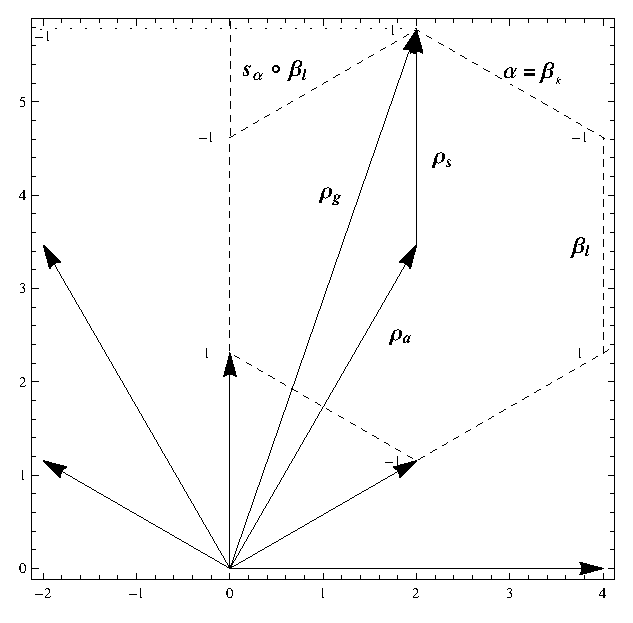
\includegraphics[width=100mm]{g2-roots}
  }
  \caption{Положительные корни $G_{2}$ и образование сингулярного элемента $\Phi^{(0)}_{\mathfrak{s}}$ в главной камере Вейля алгебры $\af=A_{2}$.}
  \label{fig:g2-roots}
\end{figure}
Здесь оба стебля метрические и соответствующие корневые системы эквивалентны. На Рисунке \ref{fig:g2-roots} показана часть сингулярного элемента $\Phi_{G_{2}}^{\left( 0\right) }$. Границы  $\bar{C_{\frak{a}}}$ изображены пунктирными линиями, начинающимися в центре сингулярного элемента. Они содержат ребро $\lambda _{2}=-\alpha _{2}=-\beta _{2}$ и корни $-\beta _{1}=-s_{\alpha _{2}}\circ \beta _{3}$ и $ -\beta _{3}$
($\beta _{3}$ показан, как $\beta _{l}$). Для корня $\beta_{1}$ искомая пара -- это  $(\alpha _{1}, \beta _{2})$: $\alpha _{1}=\beta _{1}-\beta _{2}$. Ребро $\lambda _{2,3}^{\sfr}=\beta _{3}$ равно  $\lambda _{1}^{\frak{s}}=\beta _{1}=s_{\alpha _{2}}\circ \beta _{3}$ и  $\sfr$-модуль получает индекс Дынкина $m_{1}$  и наследует второй индекс $m_{2}$. В этом частном случае  $m_{1}=m_{2}=0$.  Общий случай с начальным модулем $L^{\mu }$, где $\mu =m_{1}\omega _{1}+m_{2}\omega _{2}$, может быть рассмотрен аналогично: необходимо найти ребро $\lambda _{2}=-\left(
m_{2}+1\right) \beta _{2}$ и положить $\lambda_{1}^{\sfr}=-\left( m_{1}+1\right) \beta _{1}$, его конец принадлежит границе $\bar{C_{\af}}$. Отражение $s_{\beta_{2}} $ переводит $\beta _{1}$ в $\beta _{3}$ и соответствующее ребро
$\lambda _{2,3}^{\sfr}=-\left( m_{1}+1\right) \beta _{3}$ имеет длину $\left( m_{1}+1\right) $. Теперь рассмотрим ребра $\lambda _{1}^{\sfr}$ (или $\lambda _{2,3}^{\sfr} $) и $\lambda _{1,3}^{\sfr}$ (или $\lambda _{2,3,1}^{\sfr}$), и обнаружим, что они принадлежат границе  $\bar{C_{\af}}$ и Вейлевская симметрия предсказывает, что $\lambda _{1,3}^{\sfr}=-\left( m_{2}+1\right)\beta _{3}$ ($\lambda _{2,3,1}^{\sfr}=-\left( m_{2}+1\right) \beta _{1}$) . Наконец, ребро $\lambda _{1,3,2}^{\sfr}=-\left(m_{1}+1\right) \beta _{2}$ замыкает многогранник. Его вершины соответствуют весам сингулярного элемента $\Phi _{\sfr}^{\left( \widetilde{\mu }\right) }=\sum_{w\in W_{\sfr}}\varepsilon \left( w\right) e^{w\circ \left(
\widetilde{\mu }+\rho_{\sfr}\right) }$ модуля $L_{\sfr}^{\left( \widetilde{\mu }\right) }$, где $\widetilde{\mu }=m_{1}\widetilde{\omega }_{1}+m_{2}\widetilde{\omega }_{2}$. Заметим, что в этом случае знаковые множители можно получить прямо в первоначальной весовой системе, так как стебли метрические.
\item
Тип 1. $\Delta _{F_{4}}\approx (\Delta _{D_{4}},\Delta_{D_{4}}).$

Оба стебля здесь метрические и соответствующие корневые системы эквивалентны.  Система $\Delta _{D_{4}}$ подалгебры $\frak{a=}D_{4}$ формируется множеством $\left\{ \pm e_{i}\pm e_{j}\right\} _{|i,j=1,\ldots 4,\; i\neq j}.$ Простые корни $S_{\frak{c}}$ -- это $\left\{e_{2}-e_{3},e_{3}-e_{4}\right\} $ и $S_{\frak{d}}=\left\{ e_{4},\frac{1}{2}\left(e_{1}-e_{2}-e_{3}-e_{4}\right) \right\} $.
Для модуля $L^{\mu }$, где $\mu =\sum m_{k}\omega _{k}$ рассмотрим ребро $\lambda _{3}=-\left( m_{3}+1\right) e_{4}=-\left( m_{3}+1\right)
\beta _{3}$.
Построим ребро $\lambda _{2}^{\sfr}=-\left( \widetilde{m}_{2}+1\right) \beta _{2}$. Искомая пара корней -- это $\left(\alpha_{2}=e_{3}-e_{4},\beta _{3}\right) $. Пересечение  $\lambda _{2}^{\sfr}$ с  $\alpha _{2}$-границей камеры $\bar{C_{\af}}$ определяет длину $\lambda _{2}^{\sfr}=-\left( m_{2}+1\right) \beta _{2}$ и длины ребра $\lambda _{3,2}^{\sfr}$ равна длине $\lambda _{2}^{\sfr}$. Далее рассмотрим ребро $\lambda _{2}^{\sfr}=-\left( m_{2}+1\right) \beta _{2}$ и пару $\left( \alpha_{1}=e_{2}-e_{3},\beta _{1}=e_{2}\right) $. Длина   $\lambda _{1}^{\sfr}$ становится равной $\lambda_{1}^{\sfr}=-\left( m_{1}+1\right) \beta _{1}$. Продолжаем эту процедуру, пока не замкнем многогранник. Ребра, направленные вдоль корней типа $\alpha_4$, $\alpha _{4}=\beta_{4}=$ $\frac{1}{2}\left( e_{1}-e_{2}-e_{3}-e_{4}\right) $, рассматриваются аналогично и, наконец, сингулярный элемент $\Phi_{\sfr}^{\left( \widetilde{\mu }\right) }=\sum_{w\in W_{\sfr}}\varepsilon \left( w\right) e^{w\circ \left(\widetilde{\mu }+\rho _{\sfr}\right) }$ для модуля $L_{\sfr}^{\left( \widetilde{\mu }\right) }$, где
$\widetilde{\mu }=\sum m_{k}\widetilde{\omega }_{k}$ возникает в камере $\bar{C_{\af}}$.
\item
Тип 2. $\Delta _{B_{r}}\approx (\Delta _{D_{r}},\Delta _{\oplus^{r}A_{1}}). $

Оба стебля метрические. Вложения дается стеблем $\Delta_{D_{r}}$ с простыми корнями $S_{\af}=\left\{e_{1}-e_{2},e_{2}-e_{3},\ldots,e_{r-1}-e_{r},e_{r-1}+e_{r}\right\} $. Второй стебель соответствует прямой сумме алгебр $A_{1}$ с простыми корнями $S_{\sfr}=\left\{ e_{1},e_{2},\ldots ,e_{r-1},e_{r}\right\} $. Рассмотрим ребро $\lambda _{r}=-\left( m_{r}+1\right) \beta _{r}$ (здесь $\beta_{r}=e_{r}$) и ребро $\lambda _{r-1}=-\left(\widetilde{m}_{r-1}+1\right) \beta _{r-1}$, присоединенное к нему (здесь $\beta_{r-1}=e_{r-1}$). Соответствующая пара корней -- это $\left( \alpha _{r-1}=e_{r-1}-e_{r},\beta _{r-1}=e_{r-1}\right) $. Из условия пересечения определяется второе ребро $\lambda_{r-1}=-\left( m_{r-1}+1\right) \beta _{r-1}$ , оно ортогонально к  $\beta _{r}$, так что противоположное ребро имеет ту же длину. Индекс Дынкина $m_{r-1}$ теперь связан также с простым корнем $\beta _{r-1}$. Далее рассмотрим полученное ребро $\lambda _{r-1}=-\left( m_{r-1}+1\right) \beta _{r-1}$ и $\lambda_{r-2}=-\left( \widetilde{m}_{r-2}+1\right) \beta _{r-2}$, чтобы определить индекс $\widetilde{m}_{r-2}=m_{r-2}$ и ребро $\lambda _{r-2}=-\left( m_{r-2}+1\right) \beta _{r-2}$, и так далее, пока все пары ребер не будут определены. Наконец, в $\bar{C}_{D_{r}}$ элемент $\Phi _{\oplus ^{r}A_{1}}^{\left(\widetilde{\mu }\right) }=\sum_{w\in W_{\oplus^{r}A_{1}}}\varepsilon \left( w\right) e^{w\circ \left( \widetilde{\mu }+\frac{1}{2}\sum e_{k}\right) }$ может быть построен для модуля
$L_{\oplus ^{r}A_{1}}^{\left( \widetilde{\mu }\right) }$, где
$\widetilde{\mu }=\sum m_{k}\frac{1}{2}e_{k}$.

\item
Тип 2. $\Delta _{C_{r}}\approx (\Delta _{D_{r}},\Delta _{\oplus^{r}A_{1}}). $

Ситуация в этом случае эквивалентна предыдущему и дополнительные ребра строятся аналогично.

\item
Тип 3 $\Delta _{A_{r}}\approx (\Delta _{A_{r-1}\oplus u_{1}},\Delta _{\oplus ^{r}A_{1}}).$

Здесь только первый стебель метрический и он определяет вложение с простыми корнями  $S_{\af}=\left\{ e_{1}-e_{2},e_{2}-e_{3},\ldots ,e_{r-1}-e_{r}\right\} $. Второй стебель, соответствующий прямой сумме  $r$ копий алгебры $A_{1}$, имеет простые корни $S_{\sfr}=\left\{
e_{1}-e_{r+1},e_{2}-e_{r+1},\ldots ,e_{r}-e_{r+1}\right\} $. Рассмотрим ребро $\lambda _{r}=-\left( m_{r}+1\right) \beta _{r}$ с $\beta
_{r}=e_{r}-e_{r+1}$ и $\lambda _{r-1}=-\left( \widetilde{m}_{r-1}+1\right) \beta _{r-1}$  с $\beta_{r-1}=e_{r-1}-e_{r+1}$ присоединенным к нему. Тогда соответствующая пара равна $\left( \alpha _{r-1}=e_{r-1}-e_{r},\beta_{r-1}=e_{r-1}-e_{r+1}\right)$. Пересечение с границей $\bar{C}_{A_{r-1}}$, ортогональной $\alpha _{r-1}$ определяет второе ребро $\lambda _{r-1}=-\left(m_{r-1}+1\right) \beta _{r-1}$. Индекс Дынкина $m_{r-1}$ должен использоваться для фундаментального веса  $\omega _{r-1}.$ Отражение  $s_{\beta _{r}}$ переводит $\lambda _{r-1}=-\left(m_{r-1}+1\right) \beta _{r-1}$ в $\lambda _{r,r-1}=-\left(m_{r-1}+1\right) \beta _{r-1}.$ Далее рассмотрим полученное ребро edge
$\lambda _{r-1}=-\left( m_{r-1}+1\right) \beta _{r-1}$ и $\lambda _{r-2}=-\left( \widetilde{m}_{r-2}+1\right) \beta _{r-2}$ с  $\beta_{r-2}=e_{r-2}-e_{r+1} $ , чтобы получить индекс $\widetilde{m}_{r-2}=m_{r-2}$ и ребро $\lambda _{r-2}=-\left(m_{r-2}+1\right) \beta _{r-2}$, и так далее, пока не получим все пары ребер. Наконец, в  $\bar{C}_{D_{r}}$ элемент$\Phi _{\oplus ^{r}A_{1}}^{\left( \widetilde{\mu }\right)}=\sum_{w\in W_{\oplus^{r}A_{1}}}\varepsilon \left( w\right) e^{w\circ \left( \widetilde{\mu }+\widetilde{\rho }\right) }$ может быть построен для модуля $L_{\oplus ^{r}A_{1}}^{\left( \widetilde{\mu }\right) }$, где $\widetilde{\mu }=\sum m_{k}\beta _{k}.$ Простейший случай $\Delta _{A_{2}}\approx (\Delta _{A_{1}\oplus u_{1}},\Delta_{A_{1}\oplus A_{1}})$ показан в примере \ref{example-1} и на Рисунке \ref{fig:a2_splint}.
\item
Тип 3 $\Delta _{B_{2}}\approx (\Delta _{A_{1}},\Delta _{A_{2}}).$

Этот сплинт показан в примере \ref{example-2} и на Рисунке \ref{fig:b2_splint}, 
$S_{A\_1}=\left\{ e_{1}-e_{2}\right\} $, $S_{A\_2}=\left\{e_{1},e_{2}\right\} $. Ребро $\lambda _{\alpha _{2}}=\lambda_{\beta _{2}}=-\left( m_{2}+1\right) \beta _{2}$ продолжается ребром $\lambda _{\beta _{1}}=-\left( \widetilde{m}_{1}+1\right) \beta_{1}$. Рассмотрим пару $\left(\alpha_{1}=e_{1}-e_{2},\beta _{1}=e_{1}\right)$. Конец ребра $\lambda _{\beta _{1}}$ должен указывать вес, инвариантный по отношению к отражению  $s_{\alpha _{1}}$. Его длина таким образом фиксирована: $\lambda _{\beta _{1}}=-\left( m_{1}+1\right) \beta _{1}$ В кообразе второго стебля, то есть в корневой системе $\Delta_{A_{2}}$, отражение $s_{\beta _{2}}$ переводит $\lambda _{\beta _{1}}=-\left(m_{1}+1\right) \beta_{1}$ в $\lambda _{2,3}$, то есть это ребро имеет ту же длину в $\beta _{3}=e_{1}+e_{3}$, и $\lambda _{2,3}=-\left(m_{1}+1\right)\beta _{3}$ с $\beta_{3}=e_{1}+e_{3}$. Неприводимый  $\sfr$-модуль имеет старший вес $\widetilde{\mu }=m_{1}\widetilde{\omega }_{1}+m_{2}\widetilde{\omega }_{2}$. На Рисунке \ref{fig:b2_splint} мы видим детали этих соотношений и, в частности, случай, когда $L_{B_{2}}^{\left[ 3,2\right] }$ редуцируется на подалгебру $A_{1}\oplus u\left( 1\right) $ и соответствующие старшие веса (вместе с их кратностями) образуют диаграмму $\mathcal{N}_{A_2}^{\left[ 3,2\right] }$ .
\end{itemize}

%%%%%%%%%%%%%%%%%%%%%%%%%%%%%%%%%%%%%%%%%%%%%%%%%%%%%%%%%%%%%
%%%%%%%%%%%%%%%%%%%%%%%%%%%%%%%%%%%%%%%%%%%%%%%%%%%%%%%%%%%%%


%%
%% End of file
%%% Local Variables: 
%%% mode: latex
%%% TeX-master: "thesis"
%%% End: 

\conclusion
\label{cha:conclusion}

А карданный вал мы сделаем из дерева, потому что до сюда все равно никто не дочитает.


%%
%% End of file
%%% Local Variables: 
%%% mode: latex
%%% TeX-master: "thesis"
%%% End: 

% ----------------------------------------------------------------
\bibliography{bibliography,cpc}
\bibliographystyle{disser}
% ----------------------------------------------------------------
\appendix
\chapter{Вычислительные методы для теории представлений аффинных алгебр Ли}

\label{cha:computational-methods}
%% \newcommand{\go}{\stackrel{\circ }{\mathfrak{g}}}
%% \newcommand{\ao}{\stackrel{\circ }{\mathfrak{a}}}
%% \newcommand{\co}[1]{\stackrel{\circ }{#1}}
%% \newcommand{\pia}{\pi_{\mathfrak{a}}}
%% \newcommand{\piab}{\pi_{\mathfrak{a}_{\bot}}}
%% \newcommand{\gf}{\mathfrak{g}}
%% \newcommand{\af}{\mathfrak{a}}
%\newcommand{\bff}{\mathfrak{b}}
%% \newcommand{\afb}{\mathfrak{a}_{\bot}}
%% \newcommand{\hf}{\mathfrak{h}}
%\newcommand{\hfg}{\hf_{\gf}}
%% \newcommand{\hfb}{\mathfrak{h}_{\bot}}
%% \newcommand{\pf}{\mathfrak{p}}
%% \newcommand{\aft}{\widetilde{\mathfrak{a}}}


\begin{abstract}
%% Text of abstract
In this paper we present {\bf Affine.m} -- program for computations in representation theory of finite-dimensional and affine Lie algebras and describe implemented algorithms.  Algorithms are based on the properties of weights and Weyl symmetry. The most important problems for us are the ones, concerning computation of weight multiplicities in irreducible and Verma modules, branching of representations and tensor product decomposition. These problems have numerous applications in physics and we provide some examples of these applications. The program is implemented in popular computer algebra system {\it Mathematica} and works with finite-dimensional and affine Lie algebras. 

% A submitted program is expected to be of benefit to other physicists or physical chemists, or be an exemplar of good programming practice, or illustrate new or novel programming techniques which are of importance to some branch of computational physics or physical chemistry.
%
% Acceptable program descriptions can take different forms. The following Long Write-Up structure is a suggested structure but it is not obligatory. Actual structure will depend on the length of the program, the extent to which the algorithms or software have already been described in literature, and the detail provided in the user manual.

%Your manuscript and figure sources should be submitted through the Elsevier Editorial System (EES) by using the online submission tool at \\
% http://www.ees.elsevier.com/cpc.

%In addition to the manuscript you must supply: the program source code; job control scripts, where applicable; a README file giving the names and a brief description of all the files that make up the package and clear instructions on the installation and execution of the program; sample input and output data for at least one comprehensive test run; and, where appropriate, a user manual. These should be sent, via email as a compressed archive file, to the CPC Program Librarian at cpc@qub.ac.uk.

\end{abstract}



%%
%% Start line numbering here if you want
%%
% \linenumbers

% Computer program descriptions should contain the following
% PROGRAM SUMMARY.

{\bf PROGRAM SUMMARY}%/NEW VERSION PROGRAM SUMMARY}
  %Delete as appropriate.

\begin{small}
\noindent
{\em Manuscript Title:}{\bf Affine.m} -- {\it Mathematica} package for computations in representation theory of finite-dimensional and affine Lie algebras                                       \\
{\em Authors:}Anton Nazarov                                                \\
{\em Program Title:}Affine.m                                          \\
{\em Journal Reference:}                                      \\
  %Leave blank, supplied by Elsevier.
{\em Catalogue identifier:}                                   \\
  %Leave blank, supplied by Elsevier.
{\em Licensing provisions:}none                                   \\
  %enter "none" if CPC non-profit use license is sufficient.
{\em Programming language:}Mathematica                                   \\
{\em Computer:}i386-i686, x86\textunderscore 64                                               \\
  %Computer(s) for which program has been designed.
{\em Operating system:} Linux, Windows, MacOS, Solaris                                       \\
  %Operating system(s) for which program has been designed.
{\em RAM:} 5-500 Mb                                              \\
  %RAM in bytes required to execute program with typical data.
%{\em Number of processors used:}                              \\
  %If more than one processor.
%{\em Supplementary material:}                                 \\
  % Fill in if necessary, otherwise leave out.
{\em Keywords:} Mathematica; Lie algebra; affine Lie algebra; Kac-Moody algebra; root system; weights; irreducible modules, CFT, Integrable systems\\
  % Please give some freely chosen keywords that we can use in a
  % cumulative keyword index.
{\em Classification:} 5 Computer Algebra, 4.2 Other algebras and groups                                         \\
  %Classify using CPC Program Library Subject Index, see (
  % http://cpc.cs.qub.ac.uk/subjectIndex/SUBJECT_index.html)
  %e.g. 4.4 Feynman diagrams, 5 Computer Algebra.
%{\em External routines/libraries:}                            \\
  % Fill in if necessary, otherwise leave out.
%{\em Subprograms used:}                                       \\
  %Fill in if necessary, otherwise leave out.
%{\em Catalogue identifier of previous version:}*              \\
  %Only required for a New Version summary, otherwise leave out.
%{\em Journal reference of previous version:}*                  \\
  %Only required for a New Version summary, otherwise leave out.
%{\em Does the new version supersede the previous version?:}*   \\
  %Only required for a New Version summary, otherwise leave out.
{\em Nature of problem:}\\
  %Describe the nature of the problem here.
Representation theory of finite-dimensional Lie algebras has many applications in different branches of physics, including elementary particle physics, molecular physics, nuclear physics. Representations of affine Lie algebras appear in string theories and two-dimensional conformal field theory used for the description of critical phenomena in two-dimensional systems. Also Lie symmetries play major role in study of quantum integrable systems.
   \\
{\em Solution method:}\\
  %Describe the method solution here.
We work with weights and roots of finite-dimensional and affine Lie algebras and use Weyl symmetry extensively. Central problems which are the computations of weight multiplicities, branching and fusion coefficients are solved using one general recurrent algorithm based on generalization of Weyl character formula. We also offer alternative implementation based on Freudenthal multiplicity formula which can be faster in some cases.
   \\
%{\em Reasons for the new version:}*\\
  %Only required for a New Version summary, otherwise leave out.
%   \\
%{\em Summary of revisions:}*\\
  %Only required for a New Version summary, otherwise leave out.
%   \\
{\em Restrictions:}\\
  %Describe any restrictions on the complexity of the problem here.
Computational complexity grows fast  with the rank of algebra, so computations for algebra of rank greater than 8 are non practical.
   \\
{\em Unusual features:}\\
  %Describe any unusual features of the program/problem here.
We offer the possibility to use traditional mathematical notation for objects in representation theory of Lie algebras in computations if {\bf Affine.m} is used in {\it Mathematica} notebook interface.
   \\
%{\em Additional comments:}\\
  %Provide any additional comments here.
%   \\
{\em Running time:}\\
  %Give an indication of the typical running time here.
From seconds to days depending on rank of algebra and complexity of representations.
   \\

% \begin{thebibliography}{0}
% \bibitem{1}Reference 1         % This list should only contain those items referenced in the
% \bibitem{2}Reference 2         % Program Summary section.
% \bibitem{3}Reference 3         % Type references in text as [1], [2], etc.
%                                % This list is different from the bibliography at the end of
%                                % the Long Write-Up.
% \end{thebibliography}
% * Items marked with an asterisk are only required for new versions
% of programs previously published in the CPC Program Library.\\
\end{small}


%% main text
\section{Introduction}
\label{intro}

Representation theory of Lie algebras is of central importance for different areas of physics and mathematics. In physics Lie algebras are used to describe symmetries of quantum and classical systems. Computational methods in representation theory have a long history \cite{belinfante1989survey}, there exist numerous software packages for computations related to Lie algebras \cite{simplie}, \cite{vanleeuwen1994lsp}, \cite{stembridge1995mps,coxweyl}, \cite{fischbacher2002ilp}, \cite{Fuchs:1996dd}.

Most popular programs \cite{simplie}, \cite{vanleeuwen1994lsp}, \cite{fischbacher2002ilp}, \cite{coxweyl} are created to study representation theory of simple finite-dimensional Lie algebras. The main computational problems are the following:
\begin{enumerate}
\item Construction of root system which determine the properties of Lie algebra including its commutation relations.
\item Weyl group traversal which is important due to Weyl symmetry of root system and characters of representations.
\item Calculation of weight multiplicities, branching and fusion coefficients, which are essential for construction and study of representations.
\end{enumerate}
There are well-known algorithms for these tasks \cite{moody1982fast}, \cite{stembridge2001computational}, \cite{belinfante1989survey}, \cite{casselman1994machine}.
The third problem is most computation-intensive. There are two different recurrent algorithms which are based on the Weyl character formula and the Freudenthal multiplicity formula. In this paper we analyze them both.

Infinite-dimensional Lie algebras also have growing number of applications in physics for example in conformal field theory and in a study of  integrable systems. But infinite-dimensional algebras are much harder to investigate and the number of available computer programs is much smaller in this case.

Affine Lie algebras \cite{kac1990idl} constitute important and tractable class of infinite-dimensional Lie algebras. They are constructed as central extensions of loop algebras of (semi-simple) finite-dimensional Lie algebras and appear naturally in a study of Wess-Zumino-Witten and coset models in conformal field theory \cite{Walton:1999xc}, \cite{difrancesco1997cft}, \cite{Goddard198588}, \cite{Dunbar:1992gh}.

The structure of affine Lie algebras allows to adapt for them computational algorithms created for finite-dimensional Lie algebras  \cite{Fuchs:1996dd}, \cite{gannon2001algorithms}, \cite{kass1990ala}. The book \cite{kass1990ala} with the tables of multiplicities and other computed characteristics of affine Lie algebras and representations was published in 1990. But we are not aware of software packages for popular computer algebra systems which can be used to extend these results.
We address this issue and present {\bf Affine.m} -- {\it Mathematica} package for computations in representation theory of affine and finite-dimensional Lie algebras.  We describe the features and limitations of the package in the present paper.  We also provide representation-theoretical background of implemented algorithms and present examples of computations relevant to physical applications.

The paper starts with an overview of Lie algebras and their representation theory (Sec. \ref{sec:theor-backgr}). Then we describe datastructures of {\bf Affine.m} used to present different objects related to Lie algebras and representations (Sec. \ref{sec:core-datastructures}) and discuss implemented algorithms (Sec. \ref{sec:comp-algor}). Next section consists of physically interesting examples (Sec. \ref{sec:examples}). The paper is concluded with the discussion of possible extensions and refinements (Sec. \ref{sec:conclusion}).

\section{Theoretical background}
\label{sec:theor-backgr}

In this section we remind necessary definitions and present formulae used in computations. 

\subsection{Lie algebras of finite and affine types}
\label{sec:lie-algebras-finite}

{\it Lie algebra} $\gf$ is a vector space with bilinear operation $[\cdot,\cdot]:\gf\otimes\gf\to \gf$, which is called {\it Lie bracket}. If we choose the basis $X_{i}$ in $\gf$ we can specify commutation relations by the {\it structure constants} $C_{ijk}$:
\begin{equation}
  \label{eq:1}
  [X^{i},X^{j}]=\sum_{k} C^{ij}_{k} X^{k}
\end{equation}
Lie algebra is {\it simple} if it contains no non-trivial ideals with respect to commutator. {\it Semisimple} Lie algebra is a direct sum of simple Lie algebras. In the present paper we treat simple and semisimple Lie algebras. 

{\it Cartan subalgebra}  $\hfg$ is a nilpotent subalgebra of  $\gf$ that coincides with its normalizer. 
We denote the elements of basis of $\hfg$ by $H^{i}$.

Killing form on $\gf$ gives a non-degenerate bilinear form $(\cdot,\cdot)$ on $\hfg$ which can be used to identify $\hfg$ with the subspace of the dual space $\hfg^{*}$ of linear functionals on $\hfg$. {\it Weights} are the elements of $\hfg^{*}$ and are denoted by Greek letters $\mu,\nu, \omega, \lambda\dots$

Special choice of basis gives compact description of commutation relations (\ref{eq:1}). This basis can be encoded by the root system which is discussed in Section \ref{sec:weights-roots} (See also \cite{humphreys1997introduction,humphreys1992reflection}).

{\it Loop algebra} $L\gf=\gf\otimes \mathbb{C}[t,t^{-1}]$, corresponding to semisimple Lie algebra $\gf$, has commutation relations
\begin{equation}
  \label{eq:6}
  [X^{i}t^{n},X^{j}t^{m}]=t^{n_+m}\sum_{k}C^{ij}_{k}X^{k}
\end{equation}
Central extension leads to the appearance of an additional term
\begin{equation}
  \label{eq:7}
   [X^{i}t^{n}+\alpha c,X^{j}t^{m}+\beta c]=t^{n+m}\sum_{k}C^{ij}_{k}X^{k}+(X^{i},X^{j})n\delta_{n+m,0}c
\end{equation}
This algebra $\hat\gf=\gf\otimes\mathbb{C}[t,t^{-1}]\oplus\mathbb{C}c$ is called non-twisted {\it affine Lie algebra} \cite{kac1990idl}, \cite{wakimoto2001idl,wakimoto2001lectures}, \cite{kass1990ala}.

We do not treat twisted affine Lie algebras in the present paper.

\subsection{Modules, weights and roots}
\label{sec:weights-roots}

Let $\gf$ be a inite-dimensional or an affine Lie algebra.

Then $\gf$-module is a vector space $V$ together with a bilinear map $\gf \times V\to V$ such that
\begin{equation}
  \label{eq:2}
  [x,y]\cdot v = x\cdot(y\cdot v) - y\cdot(x\cdot v), \quad \mbox{for}\; x,y\in \gf, v\in V
\end{equation}
Representation of algebra $\gf$ on a vector space $V$ is the homomorphism $\gf\to gl(V)$ from $\gf$ to Lie algebra of endomorphisms of the  vector space $V$ with the commutator as a bracket.

For an arbitrary representation it is possible to diagonalize the operators corresponding to Cartan generators $H^{i}$ simultaneously by a special choice of basis $\{v_{j}\}$ in $V$:
\begin{equation}
  \label{eq:3}
  H^{i}\cdot v_{j}=\nu_{j}^{i}v_{j}
\end{equation}
Eigenvalues $\nu^{i}_{j}$ of Cartan generators on an element of basis $v_{j}$ determine a weight $\nu_{j}\in \hfg^{*}$ such that $\nu_{j}(H^{i})=\nu_{j}^{i}$. Vector $v\in V$ is called the weight vector of the weight $\lambda$ if $H v=\lambda_{j}(H)v,\; \forall H\in \hf$. The  weight subspace consists of all weight vectors $V_{\lambda}=\{v\in V: H v=\lambda_{j}(H)v,\; \forall H\in \hf\}$. The weight multiplicity $m_{\lambda}=\mathrm{mult}(\lambda)=\mathrm{dim} V_{\lambda}$ is the dimension of the weight subspace.

The structure of module is determined by the set of weights since the action of generators $E^{\alpha}$ on weight vectors is
\begin{equation}
  \label{eq:5}
  E^{\alpha}\cdot v_{\lambda} \propto v_{\lambda+\alpha}
\end{equation}
Module structure can be encoded by the formal character of a module
\begin{equation}
  \label{eq:10}
  \mathrm{ch}V=\sum_{\lambda}m_{\lambda} e^{\lambda}
\end{equation}
Character  $\mathrm{ch}V\in \mathcal{E}$ is an element of algebra $\mathcal{E}$ generated by formal exponents of weights.
A character can be specialized by taking its value on some element $\xi$ of $\hf$.

Lie algebra is its own module with respect to a special kind of representation. The action that
defines this representation is called adjoint and is given by the bracket $ad_{X} Y=[X,Y]$. 
{\it Roots} are weights of the adjoint representation of $\gf$. They encode the commutation relations of algebra in the following way. Denote by $\Delta$ the set of roots. For each $\alpha\in \Delta$ there exist a root $-\alpha\in \Delta$ and the generators $E^{\alpha}, E^{-\alpha}$ such that
\begin{align}
  \label{eq:4}
  &  [H^{i},E^{\alpha}]=\alpha^{i}E^{\alpha} \\
  &\left[E^{\alpha},E^{\beta}\right]=
  \begin{cases}
    N_{\alpha,\beta} E^{\alpha+\beta}, & \mbox{if}\; \alpha+\beta\in \Delta\\
    \frac{2}{(\alpha,\alpha)} \sum_{i}\alpha^{i} H^{i},&  \mbox{if}\; \alpha=-\beta\\
    0,&\mbox{otherwise}
  \end{cases}
\end{align}

Given the root system $\Delta$ we can choose the set of positive roots. This is a subset  $\Delta^{+}\subset \Delta$ such that for each root $\alpha\in\Delta$ exactly one of the roots $\alpha, -\alpha$ is contained in $\Delta^{+}$ and for any two distinct positive roots $\alpha, \beta\in \Delta^{+}$ such that $\alpha+\beta\in \Delta$ their sum is also positive $\alpha+\beta\in\Delta^{+}$.
Elements of $-\Delta^{+}$ are called negative roots.

A positive root is {\it simple} if it cannot be written as a sum of positive roots. The set of simple roots $\Phi=\left\{\alpha_{i}\right\}$ is a basis in $\hfg^{*}$ and each root can be written as $\alpha=\sum_{i}n_{i}\alpha_{i}$ with all $n_{i}$ non-negative or non-positive simultaneously. In case of a finite-dimensional Lie algebra $\gf$ simple roots are numbered from 1 to the rank of algebra $i=1,\dots,r,\quad r=\mathrm{rank}(\gf)$. By numbering simple roots with an index $i$ we introduce lexicographic ordering in the root system $\Delta$. Highest root with respect to this ordering is denoted by  $\theta=\sum_{i=1,\dots,r} a_i \alpha_i$, coefficients $a_i$ are called {\it marks}. $\theta$ is also the highest weight  of the adjoint module (See section \ref{sec:high-weight-modul}). {\it Comarcs} are the numbers equal to $a_i^{\vee}=\frac{(\alpha_i,\alpha_i)}{2} a_i$.

Although for affine Lie algebra $\hat\gf$ the set of roots $\Delta$ is infinite the set of simple roots $\Phi$ is finite and its elements are denoted by $\alpha_{0},\dots \alpha_{r}$ where $r=\mathrm{rank}(\gf)$. The roots $\alpha_1,\dots, \alpha_r$ are the roots of the underlying finite-dimensional Lie algebra $\go$. The root $\alpha_0=\delta-\theta$ is the difference of {\it imaginary root} $\delta$ and $\theta$ -- the highest root of the algebra $\go$.
Note that root multiplicity $\mathrm{mult}(\alpha)$ for an affine Lie algebra root can be greater than one.

Subalgebra  $\bff_{+}\subset \gf$ spanned by the generators $H^{i}, E^{\alpha}$ for positive roots $\alpha\in \Delta^{+}$ is called the Borel subalgebra.

{\it Parabolic subalgebra}  $\pf_{I}\supset \bff_{+}$ contains Borel subalgebra and is  generated by some subset of simple roots $\{\alpha_{j}:j\in I, I\subset \{1\dots r\}\}$. It is spanned by the subset of generators $\{H^{i}\}\cup \{E^{\alpha}:\alpha\in \Delta^{+}\}\cup \{E^{-\alpha}: \alpha\in\Delta^{+}, \alpha=\sum_{j\in I} n_{j} \alpha_{j}\}$.
{\it Regular subalgebra} $\af\subset\gf$ is determined by the root system $\Delta_{\af}$ with the set of simple roots $\{\beta_{i}, i=1,\dots,r_{\af}\}$ being a subset of set of roots $\{\alpha_{1},\dots,\alpha_{r}\}\cup \{-\theta\}$ .

The {\it Weyl group} $W_{\gf}$ is generated by reflections $\{s_{i}:\hfg^{*}\to\hfg^{*}\}$ corresponding to simple roots $\{\alpha_{i}\}$:
\begin{equation}
  \label{eq:8}
  s_{i}\cdot\lambda=\lambda-\frac{2(\alpha_{i},\lambda)}{(\alpha_{i},\alpha_{i})}\alpha_{i}
\end{equation}
Root system and characters of representation are invariant with respect to the Weyl group  action. Root system can be reconstructed from the set of simple roots by the Weyl group transformations.

Weyl groups are finite for finite-dimensional Lie algebras and finitely-generated for affine Lie algebras.

Consider an action of the element $s_{\alpha}s_{\alpha+\delta}$ of the Weyl group of affine Lie algebra  $\hat\gf$ for $\alpha$ being a simple root of the underlying finite-dimensional Lie algebra $\gf$. Using definition \eqref{eq:8} it is easy to see that $s_{\alpha}s_{\alpha+\delta} \cdot \lambda=\lambda+\frac{2}{(\alpha,\alpha)}\alpha+\left(\frac{(\alpha,\alpha)}{2 (\lambda,\delta)}+(\lambda,\alpha)\right) \delta$. So the Weyl group can be presented as a semidirect product of the Weyl group $W_{\gf}$ of $\gf$ and the set of translations corresponding to roots of $\gf$. 

A Weyl group element can be presented as a product of elementary reflections in multiple ways. Number of elementary reflections in the shortest sequence representing an element $w\in W_{\gf}$ is called the {\it length} of $w$ and is denoted by $l(w)$. We also use the notation $\epsilon(w)=(-1)^{l(w)}$ for the parity of the number of Weyl reflections generating $w$. 

Fundamental domain $\bar{C}$ for the Weyl group $W_{\gf}$ action  on $\hfg^{*}$ is determined by the requirement $\xi\in \bar{C}\Leftrightarrow (\xi,\alpha_{i})\geq 0$ for all simple roots $\alpha_{i}$. It is called a {\it main Weyl chamber}. 

The {\it Cartan matrix} $A$ is defined by products of simple roots
\begin{equation}
  \label{eq:9}
  A_{ij}=\frac{2(\alpha_{i},\alpha_{j})}{(\alpha_{j},\alpha_{j})}
\end{equation}
and can be used for a compact description of Lie algebra commutation relations in the Chevalley basis \cite{humphreys1997introduction}, \cite{fulton1991representation}, \cite{bourbaki2002lie}.

Form \eqref{eq:9} induces a basis dual  to the simple
roots basis. It is called the {\it fundamental weights basis}. We denote
its elements by $\omega_i$:
\begin{equation}
  \label{eq:20}
  \langle\omega_i,\alpha_j\rangle=\frac{2(\omega_{i},\alpha_{j})}{(\alpha_{j},\alpha_{j})}=\delta_{ij}
\end{equation}
For a finite-dimensional Lie algebra there are $r$ fundamental weights, $i=1,\dots, r$. For affine Lie algebra we have additional fundamental weight $\omega_0=\lambda$, $(\lambda,\delta)=1, \; (\lambda,\lambda)=(\delta,\delta)=0$. Other fundamental weights are equal to $\omega_i=a_i^v \omega_0 +\co{\omega_i}$, where $\co{\omega_i}$ is the fundamental weight of the finite-dimensional Lie algebra $\gf$.

 The sum of fundamental weights $\rho=\sum_{i} \omega_{i}$ is called a {\it Weyl vector}. It is an important tool in representation theory.

\subsection{Highest weight modules}
\label{sec:high-weight-modul}

We consider finitely-generated $\gf$-modules $V$ such that $V=\bigoplus_{\xi\in \hfg^{*}} V_{\xi}$, where each $V_{\xi}$ is finite-dimensional and there exists a finite set of weights $\lambda_{1},\dots \lambda_{s}$ which generates the weight system of $V$, i.e. if $\mathrm{dim}V_{\xi}\neq 0$ then $\xi=\lambda_{i}-\sum_{k=1,\dots, r} n_{k}\alpha_{k}$ where $n_{k}\in \mathbb{Z}_{+}$ (See \cite{humphreys2008representations}, \cite{carter2005lie}).

Highest weight module $V^{\mu}$ contains a single highest weight $\mu$, all the other weights are obtained by subtractions of linear combinations of simple roots $\lambda=\mu-n_{1}\alpha_{1}-\dots-n_{r}\alpha_{r},\; n_{k}\in \mathbb{Z} _{+}$.

The most simple type of highest weight modules is the Verma module
$M^{\mu}$. Its space can be defined as a module
\begin{equation}
  \label{eq:17}
  M^{\mu}=U(\gf)\underset{U(\bff_{+})}{\otimes} D^{\mu}(\bff_{+}),
\end{equation}
with respect to a multiplication in $U(\gf)$ and
$\underset{U(\bff_{+})}{\otimes}$ means that the action of elements of $U(\bff_{+})$ ``falls through'' the left part of tensor product onto the right part. Here $\bff_{+}$ is Borel subalgebra, $D^{\mu}(\bff_{+})$ is a representation of $\bff_{+}$ such that $D(E^{\alpha})=0,\; D(H)=\mu(H)$ for any positive root $\alpha$.
Elements of $\gf$ act from the left and we should commute all the elements of $\bff_{+}$ to the right, so that they can act on the space $D^{\lambda}(\bff_{+})$.

Weight multiplicities in Verma modules can be found by applying the Weyl
character formula
\begin{equation}
  \label{eq:11}
  \mathrm{ch} M^{\mu}=\frac{e^{\mu}}{\prod_{\alpha\in \Delta^{+}} \left( 1-e^{-\alpha}\right)^{\mathrm{mult}(\alpha)}}=\frac{e^{\mu}}{\sum_{w\in W} \epsilon(w) e^{w\rho-\rho}}
\end{equation}
Here we have used the Weyl denominator identity
\begin{equation}
  \label{eq:12}
  R:=\prod_{\alpha\in \Delta^{+}} \left( 1-e^{-\alpha}\right)^{\mathrm{mult}(\alpha)}=\sum_{w\in W} \epsilon(w) e^{w\rho-\rho},
\end{equation}
and $\epsilon \left( w\right) :=\det \left( w\right)$ is equal to 
the parity of the sequence of Weyl reflections generating $w$.

Verma module $M^{\mu}$ has the unique maximal submodule and the
unique nontrivial simple quotient $L^{\mu}$ which is an
{\it irreducible highest weight module}. 

Irreducible highest weight modules have no non-trivial submodules. 
The Weyl character formula for
irreducible highest weight modules is
\begin{equation}
  \label{eq:13}
  \mathrm{ch} L^{\mu}=\frac{\sum_{w\in W} \epsilon(w) e^{w(\mu+\rho)-\rho}}{\sum_{w\in W}\epsilon(w) e^{w\rho-\rho}}=\sum_{w\in W} \epsilon(w)\; \mathrm{ch} M^{w(\mu+\rho)-\rho}
\end{equation}
Thus the character of an irreducible highest weight module can be
seen as a combination of characters of Verma modules. ( This
fact is a consequence of the Bernstein-Gelfand-Gelfand resolution
(\cite{bernstein1976category,bernstein1971structure}, see also
\cite{humphreys2008representations}).)

Construction of generalized Verma modules is analogous to (\ref{eq:17}), but representation of Borel subalgebra is substituted by a representation of parabolic subalgebra $\pf_{I}\supset \bff_{+}$ generated by some subset $\{\alpha_{I}\}$ of simple roots $I\subset \{1,\dots, r\}$:
%% !!! \Delta_{p}?!
\begin{equation*}
M_{I}^{\mu}=U\left( \gf\right)\otimes _{U\left( \pf_{I}\right) }L_{\pf_{I}}^{\mu}.
\end{equation*}
Introduce a formal element $R_{I}:=\prod_{\alpha \in \Delta
^{+}\setminus \Delta _{\pf_{I}}^{+}}\left( 1-e^{-\alpha }\right)
^{\mathrm{mult}(\alpha )}$. Then the character of a generalized
Verma module can be written as
\begin{equation}
  \label{eq:18}
  \mathrm{ch}M_{I}^{\mu}=\frac{1}{R_{I}}\mathrm{ch}L_{\pf_{I}}^{\mu }.
\end{equation}


%% Define external border of irreducible representation here

We can use the Weyl character formula to obtain recurrent relations for weight multiplicities -- important tools for calculations \cite{il2010folded,kulish4sfa}. 

For irreducible highest-weight modules recurrent relations have the following form
\begin{equation}
\label{eq:14}
m_{\xi }=-\sum_{w\in W\setminus e}\epsilon (w)m_{\xi
-\left( w(\rho )-\rho \right) }+\sum_{w\in W}\epsilon
(w)\delta _{\left( w(\mu +\rho )-\rho \right) ,\xi }.
\end{equation}
Formulae for Verma and generalized Verma modules differ only in the second term on the right-hand side. In case of Verma module it is just $\delta_{\xi,\mu}$. For generalized Verma module the summation in the second term on the right-hand side of \eqref{eq:14} is over the Weyl subgroup generated by reflections corresponding to roots $\{\alpha_{I}\}$.

Other recurrent formula can be obtained from a study of Casimir
elements action on irreducible highest weight modules
\cite{humphreys1997introduction}:
\begin{equation}
  \label{eq:15}
  m_{\lambda}=\frac{2}{(\mu+\rho)^{2}-(\lambda+\rho)^{2}}\sum_{\alpha\in \Delta^{+}}\sum_{k\geq 1} (\lambda+k\alpha,\alpha)m_{\lambda+k\alpha}.
\end{equation}
It is called the Freudenthal multiplicity formula.
Note that it is applicable only to irreducible modules. 


We discuss the use of formulae \eqref{eq:14} and \eqref{eq:15} for computations in section \ref{sec:comp-algor}. 

Now consider an algebra $\gf$ and a reductive subalgebra
$\af\subset \gf$. Simple roots $\beta_{i}$ of the subalgebra $\af$
can be presented as linear combinations of $\gf$-algebra roots
$\alpha_{j}$: $\beta_{i}=\sum_{j=1,\dots,r_{\gf}}k_{j}
\alpha_{j},\ j=1,\dots,r_{\af}$.

Each irreducible $\gf$-module is also an $\af$-module, although
$L^{\mu}_{\gf}$ is in general not irreducible as $\af$-module. 
It can be
decomposed into a direct sum of irreducible $\af$-modules:
\begin{equation}
  \label{eq:16}
  L^{\mu}_{\gf}=\bigoplus_{\nu}b^{\mu}_{\nu}L^{\nu}_{\af}
\end{equation}
Coefficients in such a decomposition are called branching
coefficients. 

It is possible to calculate branching coefficients by constructing and successively  subtracting the submodules $L^{\nu}_{\af}$. 
This traditional approach has serious limitations especially in case of affine Lie algebras. We discuss them in the end of section \ref{sec:comp-algor}. 

Now we describe an alternative approach which is based on recurrent properties of branching coefficients. 
But before we proceed to these recurrent relations we need several additional definitions.

For a subalgebra $\af\subset \gf$ we introduce the subalgebra
$\afb$. Consider the root subspace $\hf_{\perp \af}^{\ast }$
orthogonal to $\hf_{\af}$,
\begin{equation*}
\hf_{\perp \af}^{\ast }:=\left\{ \eta \in \hf^{\ast }|\forall
h\in \hf_{\af};\eta \left( h\right) =0\right\} ,
\end{equation*}
and the roots (correspondingly -- positive roots) of $\gf$ orthogonal
to roots of $\af$,
\begin{eqnarray}
\Delta _{\afb} &:&=\left\{ \beta \in \Delta _{\gf}|\forall
h\in \hf_{\af};\beta \left( h\right) =0\right\} ,
\label{delta a ort} \\
\Delta _{\afb}^{+} &:&=\left\{ \beta ^{+}\in \Delta _{\gf%
}^{+}|\forall h\in \hf_{\af};\beta ^{+}\left( h\right) =0\right\} .
\notag
\end{eqnarray}
Let $W_{\afb}$ be a subgroup of $W$ generated by
reflections $w_{\beta }$ with the roots $\beta \in \Delta _{\af_{\perp
}}^{+}$. The subsystem $\Delta _{\afb}$ determines a 
subalgebra $\afb$ with the Cartan subalgebra $\hf_{\af%
_{\perp }}$.

The Cartan subalgebra $\frak{h}$ can be decomposed in the following way:  $\frak{h}=\frak{\frak{h}_{\af}}\oplus
\frak{h}_{\afb}\oplus \frak{h}_{\perp }$

We also introduce the notations
\begin{eqnarray}
\widetilde{\frak{a}_{\perp }} :=\frak{a}_{\perp }\oplus \frak{h}_{\perp }
\qquad
\widetilde{\frak{a}} :=\frak{a}\oplus \frak{h}_{\perp }.
\end{eqnarray}

For $\af$ and $\afb$ we consider the
corresponding Weyl vectors, $\rho _{\af}$ and $\rho _{\af_{\perp
}} $ and compose the so called ''defects'' $\mathcal{D}_{\af}$ and $\mathcal{%
D}_{\afb}$ of the injection:
\begin{equation}
\mathcal{D}_{\af}:=\rho _{\af}-\pi _{\af}\rho , \qquad
\mathcal{D}_{\afb}:=\rho _{\afb}-\pi _{\af%
_{\perp }}\rho .  \label{defect-ort}
\end{equation}

%%!!! Define P^+
For $\mu \in P^{+}$ consider the linked weights $\left\{ \left(
w(\mu +\rho )-\rho \right) |w\in W\right\} $ and their projections
to
$h_{\afb}^{\ast }$ additionally shifted by the defect $-%
\mathcal{D}_{\afb}$:
\begin{equation*}
\mu _{\afb}\left( w\right) :=\pi _{\afb}\left[
w(\mu +\rho )-\rho \right] -\mathcal{D}_{\afb},\quad w\in W.
\end{equation*}
Among the weights $\left\{ \mu _{\af_{\perp
}}\left( w\right) |w\in W\right\} $ one can always choose those located in
the fundamental chamber $\overline{C_{\afb}}$. Let $U$ be the
set of representatives $u$ for the classes $W/W_{\afb}$ such
that

\begin{equation}
U:=\left\{ u\in W|\quad \mu _{\afb}\left( u\right) \in
\overline{C_{\afb}}\right\} \quad .  \label{U-def}
\end{equation}
Thus we can form the subsets:
\begin{equation}
\mu _{\widetilde{\mathfrak{a}}}\left( u\right) :=\pi _{\widetilde{%
\mathfrak{a}}}\left[ u(\mu +\rho )-\rho \right] +\mathcal{D}_{\af%
_{\perp }},\quad u\in U,  \label{mu-a}
\end{equation}
and
\begin{equation}
\mu _{\afb}\left( u\right) :=\pi _{\afb}\left[
u(\mu +\rho )-\rho \right] -\mathcal{D}_{\afb},\quad u\in U.
\label{mu-a-tilda}
\end{equation}

Notice that the subalgebra $\mathfrak{a}_{\bot}$ is regular by definition
since it is built on a subset of roots of the algebra $\mathfrak{g}$.

Denote by  $k_{\xi }^{\left( \mu \right) }$ signed branching coefficients. If $\xi\in \bar C_{\af}$ is in main Weyl chamber $k_{\xi}^{(\mu)}=b^{(\mu)}_{\xi}$ otherwise $k_{\xi}^{(\mu)}=\epsilon(w) b^{(\mu)}_{w (\xi+\rho_{\af})-\rho_{\af}}$ where $w\in W_{\af}$ is such that $w (\xi+\rho_{\af})-\rho_{\af}\in \bar C_{\af}$. 

Now we can use the Weyl character formula to write a
recurrent relation \cite{2010arXiv1007.0318L} for signed branching
coefficients $k_{\xi }^{\left( \mu \right) }$ corresponding to an
injection $\af\hookrightarrow \gf$:
\begin{equation}
\begin{array}{c}
k_{\xi }^{\left( \mu \right) }=-\frac{1}{s\left( \gamma _{0}\right) }\left(
\sum_{u\in U}\epsilon (u)\;\dim \left( L_{\afb}^{\mu _{\af%
_{\perp }}\left( u\right) }\right) \delta _{\xi -\gamma _{0},\pi _{%
\widetilde{\af}}(u(\mu +\rho )-\rho )}+\right.  \\
\left. +\sum_{\gamma \in \Gamma _{\widetilde{\af}\rightarrow \gf%
}}s\left( \gamma +\gamma _{0}\right) k_{\xi +\gamma }^{\left( \mu \right)
}\right) .
\end{array}
\label{recurrent-rel}
\end{equation}
The recursion is governed by the set $\Gamma _{\af\rightarrow \gf}$ called the injection fan. The latter is defined by the
carrier set $\left\{ \xi \right\} _{\af\rightarrow \gf}$ for the
coefficient function $s(\xi )$
\begin{equation*}
\left\{ \xi \right\} _{\widetilde{\af}\rightarrow \gf}:=\left\{
\xi \in P_{\widetilde{\af}}|s(\xi )\neq 0\right\}
\end{equation*}
appearing in the expansion
\begin{equation}
\prod_{\alpha \in \Delta ^{+}\setminus \Delta _{\bot }^{+}}\left( 1-e^{-\pi
_{\widetilde{\af}}\alpha }\right) ^{\mathrm{mult}(\alpha )-\mathrm{mult}%
_{\af}(\pi _{\widetilde{\af}}\alpha )}=-\sum_{\gamma \in P_{%
\widetilde{\af}}}s(\gamma )e^{-\gamma };\quad
\end{equation}
The weights in $\left\{ \xi \right\} _{\widetilde{\af}\rightarrow \gf}$ are to be shifted by $\gamma _{0}$ -- the lowest vector in $\left\{ \xi
\right\} $ -- and the zero element is to be eliminated:
\begin{equation}
\Gamma _{\af\rightarrow \gf}=\left\{ \xi -\gamma
_{0}|\xi \in \left\{ \xi \right\} \right\} \setminus \left\{ 0\right\} .
\end{equation}
Formula (\ref{eq:14}) is a particular case of recurrent relation for branching coefficients (\ref{recurrent-rel}) in the case of Cartan subalgebra $\af=\hfg$.

If the root system of $\afb$ is generated by some subset of $\gf$
simple roots $\alpha_{1},\dots,\alpha_{r}$ then the recurrent
relation (\ref{recurrent-rel}) is connected with the generalized
Bernstein-Bernstein-Gelfand resolution for parabolic Verma modules
\cite{2011arXiv1102.1702L}.

Another particular case of this formula is connected with tensor
product decompositions. Consider the tensor product of two
irreducible $\gf$-modules $L^{\mu}\otimes L^{\nu}$. It is also a
$\gf$-module but not irreducible in general. So
\begin{equation}
  \label{eq:19}
  L^{\mu}\otimes L^{\nu}=\bigoplus_{\gamma} f^{\mu\nu}_{\gamma}L^{\gamma}
\end{equation}
The coefficients $f^{\mu\nu}_{\gamma}$ are called fusion
coefficients. The problem of computation of fusion coefficients is
equivalent to branching problem for the diagonal subalgebra
$\gf\subset \gf\oplus \gf$ (see \cite{LyakhovskyPostnova2011}). So our implementation of recurrent algorithm can be used to decompose tensor products (See Section \ref{sec:tens-prod-decomp}).

In the case of affine Lie algebras $\gf, \af$  the multiplicities
$m_{\nu}$ and the corresponding branching coefficients $b_{\nu}$
can be regarded as the coefficients in power series decomposition
of string and branching functions correspondingly:
\begin{align}
  \label{eq:21}
  &\sigma_{\nu}(q)=\sum_{n=0}^{\infty} m_{\nu-n\delta} q^n, \quad \nu=\sum_j c_j \omega_j,\quad c_j\geq 0\\
  & b_{\nu}(q)=\sum_{n=0}^{\infty} b_{\nu-n\delta} q^n,\quad  \nu=\sum_j c_j \omega_j, \quad c_j\geq 0
\end{align}
String and branching functions have  modular and analytic properties which are important for conformal field theory, especially in  coset models and the study of CFT on higher genus surfaces \cite{kac1988modular}, \cite{difrancesco1997cft}, \cite{Walton:1999xc}, \cite{walton1989conformal}.


{\bf Affine.m}  calculates weight multiplicities and branching coefficients for affine Lie algebras up to some finite grade. We present examples of computations in Sections \ref{sec:string-funct-affine}, \ref{sec:branch-funct-coset}. Now we proceed to the description of datastructures and algorithms implemented in {\bf Affine.m}.

\section{Core datastructures}
\label{sec:core-datastructures} Having introduced necessary
mathematical objects, problems and relations we now describe the
related datastructures of {\bf Affine.m}. Although {\it
Mathematica} is untyped language it is possible to create
structured objects and do type checks with patterns
\cite{shifrinmathematica}, \cite{maeder2000computer}.
\subsection{Weights}
\label{sec:weights}

Weights are represented  by two data-structures: \lstinline{finiteWeight} for finite-dimensional Lie algebras and \lstinline{affineWeight}  for affine.

Internally the finite weight is a \lstinline{List} with the
\lstinline{Head} \lstinline{finiteWeight}, its components are the
coordinates of the weight in the orthogonal Bourbaki  basis
\cite{bourbaki2002lie}.

Affine weight is an extension of a finite weight by supplying it
with level and grade coordinates. There is a set of functions
defined for finite and affine weights. The complete list can be
found in  online help of the package. The most important
are definitions of addition, multiplication by a number and a
scalar product (bilinear form) for weights. These definitions
allow to use traditional notation when working with {\bf
Affine.m}:
\begin{lstlisting}
  w=makeFiniteWeight[{1,0,3}];
  v=makeFiniteWeight[{3,2,1}];
  2*w+v==makeFiniteWeight[{5,2,7}]
  w.v==6
\end{lstlisting}

The use of orthogonal basis in the internal structure of weights allows us to work with weights without complete specification of root system which is useful for study of branching, since roots of the subalgebra can be specified by hand.

\subsection{Root systems}
\label{sec:root-systems}

To specify an algebra of finite or affine type it is enough to fix
its root system. Root systems are represented by two datatypes
\lstinline{finiteRootSystem} and \lstinline{affineRootSystem}. The
latter is an extension of the former. We offer several different
constructors for these datastructures. It is possible to specify
the set of simple roots explicitly, for example to study the
subalgebra $B_2\subset B_4$ we can use the definition
\begin{lstlisting}
  b2b4=makeFiniteRootSystem[ { {1,-1,0,0}, {0,1,0,0} } ]
\end{lstlisting}
There are constructors for root systems of simple finite-dimensional Lie algebras:
\begin{lstlisting}
  b2=makeSimpleRootSystem[B,2]
\end{lstlisting}
We use typographic features of {\it Mathematica} frontend to offer mathematical notation for simple Lie algebras:


\begin{lstlisting}[mathescape=true]
  $B_2$ == makeFiniteRootSystem[ { {1, -1}, {0, 1} }]
\end{lstlisting}

Non-twisted affine root systems can be created as affine extensions of finte root systems, e.g.
\begin{lstlisting}
  b2affine = makeAffineExtension[b2]
\end{lstlisting}
In notebook interface this can be written simply as $\hat{B}_2$.

Semisimple Lie algebras can be created as sums of simple:
\begin{lstlisting}[mathescape=true]
  $A_1\oplus A_1$ == finiteRootSystem[2, 2, {finiteWeight[2, {1, 0}], finiteWeight[2, {0, 1}]}]
\end{lstlisting}
%% The problem is here

Predicate \lstinline{rootSystemQ} checks if the object is root systems of finite or affine type.

List of simple roots is the property of root system so it is accessed as \lstinline{rs[simpleRoots]}.

We have implemented several functions to get major properties of root systems. Weyl vector is given by the function \lstinline{rho[rs_?rootSystemQ]}:
\begin{lstlisting}[label=list:1]
  In[1]  =  rho[b2]
  Out[1]  =  finiteWeight[2, {3/2, 1/2}]
\end{lstlisting}
Positive roots can be constructed with \lstinline{positiveRoots[rs_?rootSystemQ]}. For an affine Lie algebra this and related functions return the list up to fixed grade. This grade limit is set through the value of \lstinline{rs[gradeLimit]} which is equal to 10 by default. List of roots (up to \lstinline{gradeLimit}) is returned by \lstinline{roots[rs]}. Cartan matrix and fundamental weights are calculated by the functions \lstinline{cartanMatrix} and \lstinline{fundamentalWeights} correspondingly.

It is possible to specify a weight of a Lie algebra by its Dynkin labels
\begin{lstlisting}
  weight[b2][1,2] == makeFiniteWeight[{2, 1}]
\end{lstlisting}
The function \lstinline{dynkinLabels[rs_?rootSystemQ][wg_?weightQ]} returns Dynkin labels of weight \lstinline{wg} in the root system \lstinline{rs}.

Elements of Weyl group are specified by the set of indices of reflections, so the element  $w=s_{1}s_{2}s_{1}$ of the Weyl group of algebra $B_{2}$ is constructed with \lstinline{weylGroupElement[b2][1,2,1]}. Then it can be applied to the weights:
\begin{lstlisting}
  w = weylGroupElement[b2][1,2,1];
  w @ makeFiniteWeight[{1,0}] == makeFiniteWeight[{-1,0}]
\end{lstlisting}

Computation of lexicographically minimal form \cite{casselman1994machine,casselman1995automata} for Weyl group elements can be conveniently implemented through the use of pattern-matching in {\it Mathematica}. In \cite{KallenShortlex} rewrite rules for simple finite dimensional and affine Lie algebras are presented as {\it Mathematica} patterns. Our presentation of Weyl group elements is compatible with the code of \cite{KallenShortlex}
\begin{lstlisting}[mathescape=true]
  In[1]  = $<<$A3reduce;
           reduce[s[1,2,1,2,1,3,2,1,1]]
  Out[1] = s[2, 3, 2]

  In[2]  = (weylGroupElement[$A_{3}$] @@ reduce[s[1,2,1,2,1,3,2,1,1]]) @ weight[$A_{3}$][-1,-2,-1]
  Out[2] = finiteWeight[4, {-2, 2, 1, -1}]

  In[3]  = dynkinLabels[$A_{3}$][Out[2]]
  Out[3] = {-4, 1, 2}
\end{lstlisting}

\subsection{Formal elements}
\label{sec:formal-elements}

We represent formal characters of representations by special structure \lstinline{formalElement}. This structure is a hash-table implemented with \lstinline{DownValues}. The keys are weights at the exponents and the values are the  corresponding multiplicities. \lstinline[mathescape=true]!makeFormalElement[{$\gamma_{1},\dots,\gamma_{n}$},{$m_{1},\dots,m_{n}$}]! creates data-structure which represents the element $\sum_{i=1}^{n} m_{i} e^{\gamma_{i}}$ of the formal algebra $\mathcal{E}$. The operations in $\mathcal{E}$ are implemented for \lstinline{formalElement} data-type: formal elements can be added, multiplied by a number or by an exponent of a weight. There exists also a multiplication of formal elements but no division.
\begin{lstlisting}[mathescape=true]
  In[1]  = makeFormalElement[{makeFiniteWeight[{1,1}],makeFiniteWeight[{0,0}]},{1,2}] *
             (2 * Exp[makeFiniteWeight[{1,0}]] *
             makeFormalElement[{makeFiniteWeight[{1,1}],makeFiniteWeight[{0,0}]},{1,2}]);
  In[2]  = In[1][weights]
  Out[2] = {finiteWeight[2, {1, 0}], finiteWeight[2, {2, 1}], finiteWeight[2, {3, 2}]}

  In[3]  = In[1][multiplicities]
  Out[3] = {8, 8, 2}
\end{lstlisting}

\subsection{Modules}
\label{sec:modules}

{\bf Affine.m} can be used to study different kinds of modules, i.e. Verma modules, irreducible modules and parabolic Verma modules.  We need datastructure \lstinline{module} to represent generic module of Lie algebra $\gf$. Module properties can be deduced from its set of singular weights using Weyl character formulae \eqref{eq:11},\eqref{eq:12},\eqref{eq:18},\eqref{eq:13}. Set of singular weights can have Weyl symmetry. It can be a symmetry with respect to the Weyl group $W_{\gf}$ or with respect to some subalgebra $W_{\af}$ as in the case of parabolic Verma modules. Then it is possible to study only the main Weyl chamber $C_{\af}$. To use this symmetry generic constructor for \lstinline{module} datastructure accepts several parameters \lstinline{makeModule[rs_?rootSystemQ][singWeights_formalElement,subs_?rootSystemQ|emptyRootSystem[],limit:10}. Here \lstinline{rs} is the root system of the Lie algebra $\gf$,\lstinline{singWeights} is the set of singular weights,  \lstinline{subs} is the root system corresponding to the Weyl group $W_{\af}$ which is the (anti-)symmetry of the set of singular weights. Parameter \lstinline{limit} limits computation for infinite-dimensional modules such as Verma or parabolic Verma.
There are several specialized constructors for different types of highest weight modules:
\begin{lstlisting}[mathescape=true]
vm=makeVermaModule[$B_{2}$][{2,1}];
pm=makeParabolicVermaModule[$B_{2}$][weight[$B_{2}$][2,1],{1}];
im=makeIrreducibleModule[$B_{2}$][2,1];
GraphicsRow[textPlot/@{im,vm,pm}]
$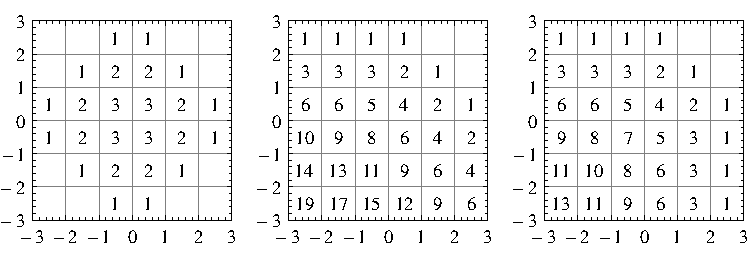
\includegraphics[width=130mm]{figures/irrep-verma-pverma}$
\end{lstlisting}

As we already stated properties of a module are encoded by its singular element. Function \lstinline{singularElement[m_module]} returns singular element of a module as \lstinline{formalElement} datastructure. Character (up to \lstinline{limit} for (parabolic) Verma modules) is returned by the function \lstinline{character[m_module]}. Direct sum of modules is a module and we use natural notation
\begin{lstlisting}[mathescape=true]
im1=makeIrreducibleModule[$B_{2}$][weight[$B_{2}$][2,1]];
im2=makeIrreducibleModule[$B_{2}$][weight[$B_{2}$][1,2]];
textPlot[im1$\oplus$ im2]
$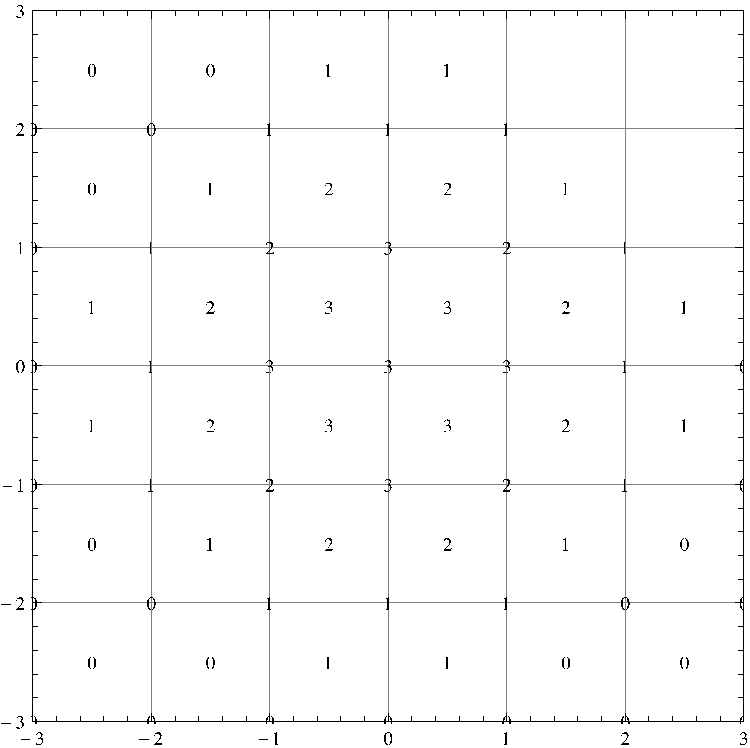
\includegraphics[width=60mm]{figures/irrep-sum}$
\end{lstlisting}

The tensor product is also implemented but only for finite-dimensional Lie algebras, since tensor product of affine Lie algebra modules leads to rich new structures \cite{kazhdan1994tensor3,kazhdan1993tensor1,kazhdan1993tensor2} which are out of the scope of the present paper.
\begin{lstlisting}[mathescape=true]
textPlot[makeIrreducibleModule[$A_{1}$][5]$\otimes$ makeIrreducibleModule[$A_{1}$][3]];
$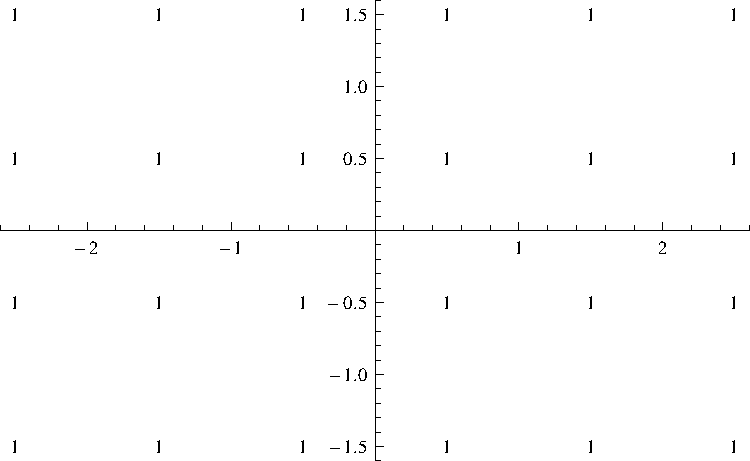
\includegraphics[width=60mm]{figures/tensor-product}$
\end{lstlisting}
\section{Computational algorithms}
\label{sec:comp-algor}
   
As we have already stated in section \ref{sec:high-weight-modul} there exist two recurrent relations which can be used to calculate weight multiplicities in irreducible modules. Both algorithms proceed in the following way to calculate weight multiplicities:
\begin{enumerate}
\item Create the list of weights in the main Weyl chamber by subtracting all possible combinations of simple roots from the highest weight (e.g. for finite-dimensional algebra subtract $\alpha_{1}$ from $\mu$ while inside $\bar C$, then subtract $\alpha_{2}$ from all the weights already obtained etc).
\item Sort the list of weights by their product with the Weyl vector.
\item Use a recurrent formula. If the weight required for recurrent computation is outside the main chamber use the Weyl symmetry.
\end{enumerate}
The difference in the performance of algorithms is in the number of previous values required to get the multiplicity of weight under consideration. For  the Weyl formula based recurrent relation \eqref{eq:14} it is constant and equal to the number of elements in the Weyl group (if we are far from the boundary of representation diagram). When the Freudenthal formula \eqref{eq:15} is used number of previous values grows with the distance from the external border of representation. So the Freudenthal formula is faster if the weight is close to the border or the rank of the algebra and the size of Weyl group is large \cite{moody1982fast}.
Note that the Freudenthal formula is valid for irreducible modules only, so it can not be used to study (generalized) Verma modules.

We have made some experiments with our implementations of the Freudenthal formula and formula \eqref{eq:15} and have got Figure  \ref{fig:freudenthal-racah-times}, which depicts the dependence of the computation time on the number of weights in a module.

\begin{figure}[h]
  \noindent\centering{
    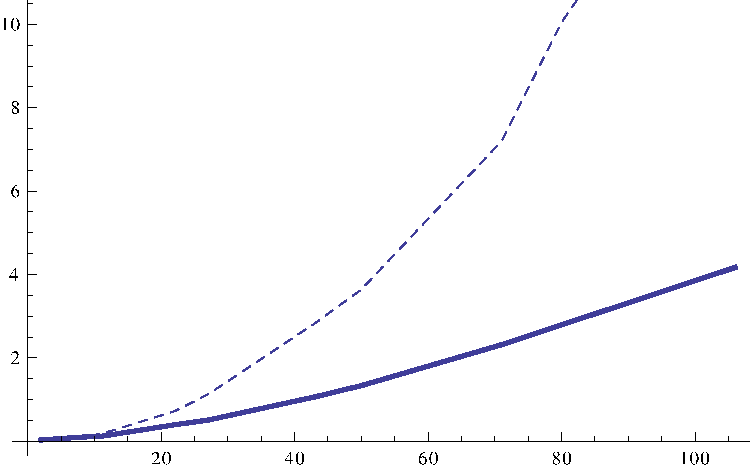
\includegraphics[width=80mm]{figures/timing}
  }
  \caption{Running time of algorithms based on the Freudenthal formula \eqref{eq:15} (dashed) and recurrent relation \eqref{eq:14} (solid) with the number of weights in $\bar C$ for calculation of multiplicities in representations of $B_{2}$.}
\label{fig:freudenthal-racah-times}

\end{figure}

In the calculation of branching coefficients the application of the Freudenthal formula requires a complete construction of formal characters of an algebra module and all the representations of a subalgebra. It is impractical when the rank of algebra and subalgebra are big, for example for maximal subalgebras.

Alternative algorithm which was presented in the paper \cite{2010arXiv1007.0318L}  contains the following steps:

\begin{enumerate}
\item  Construct the root system $\Delta _{\af}$ for the embedding $%
\af\rightarrow \frak{g}$.

\item  Select all the positive roots $\alpha \in \Delta ^{+}$ orthogonal
to  $\af$, i.e. form the set $\Delta_{\afb }^{+}$.

\item  Construct the set $\Gamma _{\af\rightarrow \frak{g}}$. Relation
 (\ref{eq:6}) defines the sign function
 $s(\gamma)$ and the set $\Phi_{\af\subset \frak{g}}$ where the lowest weight
 $\gamma_0$ is to be subtracted to get the fan:
 $\Gamma _{\af\rightarrow \frak{g}}=\left\{ \xi -\gamma _{0}|\xi \in \Phi _{%
\af\subset \frak{g}}\right\} \setminus \left\{ 0\right\}$.

\item  Construct the set $\widehat{\Psi ^{(\mu )}}=\left\{ w (\mu +\rho
)-\rho ;\;w \in W\right\} $ of singular weights for the $\frak{g}$%
-module $L^{(\mu )}$.

\item  Select the weights $\left\{ \mu _{\widetilde{\af_{\perp }}%
}\left( w\right) =\pi _{\widetilde{\af_{\perp }}}\left[ w(\mu +\rho
)-\rho \right] -\mathcal{D}_{\af_{\perp }}\in \overline{C_{\widetilde{%
\af_{\perp }}}}\right\} $. Since the set $\Delta_{\afb }^{+}$ is fixed
we can easily check wether the weight $\mu _{\widetilde{\af_{\perp }}%
}\left( w\right) $ belongs to the main Weyl chamber $\overline{C_{\widetilde{%
\af_{\perp }}}}$ (by computing its scalar product with the fundamental
weights of $\afb^{+}$).

\item  For the weights $\mu _{\widetilde{\af_{\perp }}}\left( w\right) $
calculate dimensions of the corresponding modules, $\mathrm{\dim }\left(
L_{\widetilde{\af_{\perp }}}^{\mu _{\widetilde{\af_{\perp }}%
}\left( u\right) }\right) $, using the Weyl dimension formula and construct
the singular element $\Psi ^{\left( \mu \right) }_{\left(  \af, \afb \right)}$.

\item  Calculate the anomalous branching coefficients using 
recurrent relation (\ref{recurrent-rel}) and select among them those
corresponding to the weights in the main Weyl
chamber $\overline{C_{\af}}$.
\end{enumerate}

We can speed up the algorithm by
one-time computation of the representatives of the conjugate classes $%
W/W_{\afb }$.


Consider the regular embedding $B_{2}\subset B_{4}$. In this case the fan consists of 24 elements. In order to decompose $B_{4}$ module we need to construct the subset of singular weights of the module which projects to the main Weyl chamber of the subalgebra $B_{2}$. The full set of singular weights consists of 384 elements. The required subset contains at most 48 elements. So the time for the construction of this required subset is negligible if the number of branching coefficients is greater than that. We may estimate the total number of required operations for the computation of branching coefficients as the product of the number of elements in the main Weyl chamber of a subalgebra with non-zero branching coefficients and the number of elements in the fan. In the case of a direct algorithm we need to compute the multiplicities for each module in the decomposition, so the number of operations grows faster than the square of the number of elements in the main Weyl chamber of a subalgebra with non-zero branching coefficients. 

To further illustrate this performance issue we include Figure \ref{fig:branching} where we show the time required for computations of branching coefficients for $B_{3}\subset B_{4}$.

\begin{figure}[h]
  \noindent\centering{
   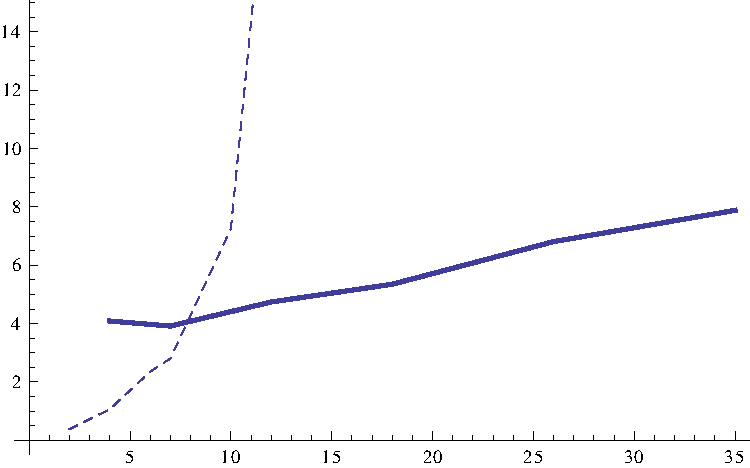
\includegraphics[width=100mm]{figures/branching-timing}
  }
  \caption{Running time of algorithms based on the Freudenthal formula \eqref{eq:15} (dashed) and recurrent relation \eqref{recurrent-rel} (solid) with the number of weights in $\bar C$ for calculation of branching coefficients for $B_{3}\subset B_{4}$.}
  \label{fig:branching}
\end{figure}

\section{Examples}
\label{sec:examples}
In this section we present some examples of computations available with {\bf Affine.m} with the code required to produce these results.

\subsection{Tensor product decompositon for finite-dimensional Lie algebras}
\label{sec:tens-prod-decomp}

Computation of fusion coefficients for the decomposition of tensor product of highest-weight modules to the direct sum of irreducible modules has numerous applications in physics. For example, we can consider the spin of a composite system such as an atom. Another interesting example is integrable spin chain consisting of $N$ particles with the spins living in some representation $L$ of a Lie algebra $\gf$ with a $\gf$-invariant Hamiltonian $H$, describing the nearest-neighbour spin-spin interaction. In order to solve such a system, i.e. to find eigenstates of the Hamiltonian, we need to decompose $L^{\otimes N}$ into the direct sum of irreducible $\gf$-modules of lower dimension and diagonalize the Hamiltonian on these modules.

For fundamental representations of simple Lie algebras it is sometimes possible to get an analytic result describing the dependence of decomposition coefficients on $N$ (See \cite{LyakhovskyPostnova2011}). Our code provides numerical values and can be used to check this analytic results.

Consider a tensor power of $B_{2}$ the first fundamental representation $\left(L^{[1,0]}\right)^{\otimes 4}$. Decomposition coefficients are just the branching
 coefficients for the tensor power module reduced to the diagonal subalgebra $B_{2}\subset B_{2}\oplus B_{2}\oplus B_{2}\oplus B_{2}$. So the following code calculates these coefficients:
\begin{lstlisting}[mathescape=true]
fm = makeIrreducibleModule[$B_{2}$][1, 0];
tp = ((fm$\otimes$ ]fm)$\otimes$ fm)$\otimes$]fm;
subs = makeFiniteRootSystem[
  {1/4*{1, -1, 1, -1, 1, -1, 1, -1}, 
   1/4*{0, 1, 0, 1, 0, 1, 0, 1}}];
bc = branching[tp, subs];
{bc[#], dynkinLabels[subs][#]} & /@ bc[weights]
\end{lstlisting}
It produces a list of highest weights and tensor product decomposition coefficients:
\begin{lstlisting}
{{1, {4, 0}}, {3, {2, 2}}, {0, {3, 0}}, 
{2, {0, 4}}, {3, {1, 2}}, {6, {2, 0}}, 
{6, {0, 2}}, {1, {1, 0}}, {3, {0, 0}}}]
\end{lstlisting}

Returning to the problem of spin chain Hamiltonian diagonalization we can see that instead of diagonalizing operator in space of dimension $625$ we can diagonalize operators in the spaces of dimensions $55, 81, 30, 35, 35, 14, 10, 5, 1$.

\subsection{Branching and parabolic Verma modules}
\label{sec:branch-parab-verma}

We illustrate the generalized BGG-resolution by the diagrams of $G_{2}$ parabolic Verma modules which appear in the decomposition of irreducible module $L^{[1,1]}_{G_{2}}$:
\begin{equation}
\mathrm{ch}\left( L^{\mu }\right) =\sum_{u\in U}\;e^{\mu _{\aft}\left(
u\right) }\epsilon (u)\mathrm{ch}M_{I}^{\mu _{\frak{a}_{\perp }}\left(
u\right) }.  \label{char-in-gen-verma-mod}
\end{equation}
The character of $L^{[1,1]}$ is presented in Figure \ref{branching-bgg}, characters of the generalized Verma modules in decomposition \eqref{char-in-gen-verma-mod} are shown in Figure \ref{g2-pverma}. Characters in the upper row appear in \eqref{char-in-gen-verma-mod} with positive sign and in the lower row -- with negative.


\begin{figure}[h]
  \noindent\centering{
    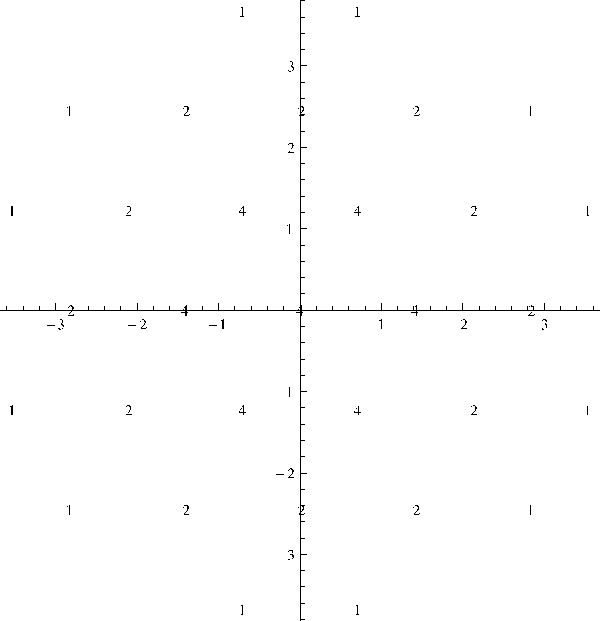
\includegraphics[width=80mm]{figures/G2-irrep}
  }
  \caption{Character of the irreducible $G_{2}$-module $L^{[1,1]}$}
  \label{branching-bgg}
\end{figure}
\begin{figure}[h]
  \noindent\centering{
    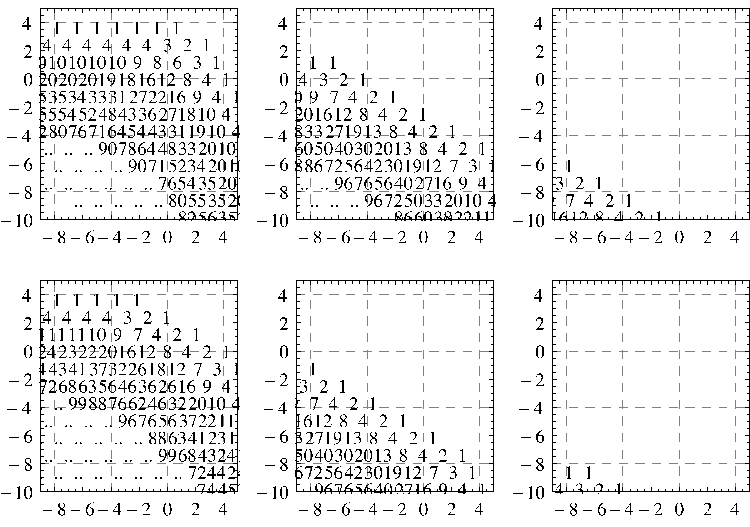
\includegraphics[width=150mm]{figures/G2-pverma}
  }
  \caption{Characters of $G_{2}$ generalized Verma modules appearing in the decomposition of $L^{[1,1]}$. Parabolic Verma modules in the upper row appear in the decomposition with a positive sign, in the lower row -- with a negative.}
  \label{g2-pverma}
\end{figure}

\subsection{String functions of affine Lie algebras and CFT models}
\label{sec:string-funct-affine}

String functions can be used to present formal characters of affine Lie algebra highest weight representation. They have interesting analytic and modular properties \cite{kac1990idl,kac1988modular,kac1984infinite}.

{\bf Affine.m} produces power series decomposition for string functions. Consider an affine Lie algebra $\hat{sl(3)}=\hat A_{2}$ and its highest weight module $L^{(1,0,0)}$. To get the string functions we can use the code:
\begin{lstlisting}[mathescape=true]
stringFunctions[$\hat A_2$,{1,1,2}]
{{0, 0, 4}, 
  $2 q + 10 q^2 + 40 q^3 + 133 q^4 + 398 q^5 + 1084 q^6 + 2760 q^7 + 6632 q^8 + 15214 q^9 + 33508 q^{10}$}, 
{{0, 3, 1}, 
  $2 q + 12 q^2 + 49 q^3 + 166 q^4 + 494 q^5 + 1340 q^6 + 3387 q^7 + 8086 q^8 + 18415 q^9 + 40302 q^{10}$}, 
{{1, 1, 2}, 
  $1 + 6 q + 27 q^2 + 96 q^3 + 298 q^4 + 836 q^5 + 2173 q^6 + 5310 q^7 + 12341 q^8 + 27486 q^9 + 59029 q^{10}$}, 
{{2, 2, 0}, 
  $1 + 8 q + 35 q^2 + 124 q^3 + 379 q^4 + 1052 q^5 + 2700 q^6 + 6536 q^7 + 15047 q^8 + 33248 q^9 + 70877 q^{10}$}, 
{{3, 0, 1}, 
  $2 + 12 q + 49 q^2 + 166 q^3 + 494 q^4 + 1340 q^5 + 3387 q^6 + 8086 q^7 + 18415 q^8 + 40302 q^9 + 85226 q^{10}$}
\end{lstlisting}
Similarly for the affine Lie algebra $\hat G_{2}$ we get
\begin{lstlisting}[mathescape=true]
stringFunctions[$\hat G_2$,{1,1,0}]
{{2, 0, 0}, 
  $1 + 8 q + 37 q^2 + 138 q^3 + 431 q^4 + 1227 q^5 + 3208 q^6 + 7901 q^7$}, 
{{0, 0, 1}, 
  $3 q + 18 q^2 + 73 q^3 + 247 q^4 + 736 q^5 + 2000 q^6 + 5070 q^7$}, 
{{1, 1, 0},
  $1 + 7 q + 32 q^2 + 117 q^3 + 370 q^4 + 1055 q^5 + 2780 q^6 + 6880 q^7$}, 
{{0, 2, 0}, 
  $3 q + 15 q^2 + 63 q^3 + 210 q^4 + 633 q^5 + 1725 q^6 + 4407 q^7$}
\end{lstlisting}

\subsection{Branching functions and coset models of conformal field theory}
\label{sec:branch-funct-coset}

It is believed that most rational models of CFT can be obtained from cosets $G/A$ corresponding to the embedding $\af\subset\gf$. These models can be studied as gauge theories \cite{Hwang:1994yr, hwang1993brst}.

Branching functions for an embedding $\af\subset\gf$ are the partition functions of CFT on the torus (see \cite{difrancesco1997cft}).

As a first example we show how to construct branching functions for the embedding $\hat A_{1}\to \hat B_{2}$ up to the tenth grade:
\begin{lstlisting}[mathescape=true]
branchingFunctions[$\hat B_{2}$,makeAffineExtension[makeFiniteRootSystem[{{1, 1}}]], {1, 1, 1}]

 {{3, 0}, 
  $2 + 14 q + 52 q^2 + 154 q^3 + 410 q^4 + 994 q^5 + 2248 q^6 + 4832 q^7 + 9934 q^8 + 19680 q^9 + 37802 q^{10}$},
 {{2, 1}, 
  $4 + 20 q + 72 q^2 + 220 q^3 + 584 q^4 + 1424 q^5 + 3248 q^6 + 7012 q^7 + 14488 q^8 + 28844 q^9 + 55616 q^{10}$},
 {{0, 3}, 
  $4 q + 20 q^2 + 68 q^3 + 200 q^4 + 516 q^5 + 1224 q^6 + 2736 q^7 + 5808 q^8 + 11820 q^9 + 23236 q^{10}$},
 {{1, 2}, 
  $2 + 14 q + 54 q^2 + 168 q^3 + 462 q^4 + 1148 q^5 + 2656 q^6 + 5812 q^7 + 12130 q^8 + 24358 q^9 + 47328 q^{10}$}
\end{lstlisting}

Another example demonstrates the computation of branching functions for the regular embedding $\hat B_{2}\subset \hat C_{3}$:
\begin{lstlisting}[mathescape=true]
sub=makeAffineExtension[parabolicSubalgebra[$C_{3}$][2,3]];
branchingFunctions[$\hat C_{3}$,sub, {2, 0, 0, 0}]

{{0, 1, 0}, 
  $2 q - 20 q^3 + 24 q^4 + 82 q^5 - 320 q^6 + 108 q^7$}, 
{{1, 0, 0}, 
  $1 - q - 8 q^2 + 19 q^3 + 16 q^4 - 156 q^5 + 205 q^6 + 640 q^7$}, 
{{0, 0, 1}, 
  $q - 5 q^3 + 7 q^5$}
\end{lstlisting}

\section{Conclusion}
\label{sec:conclusion}
We have presented the package {\bf Affine.m} for computations in representation theory of finite-dimensional and affine Lie algebras. It can be used to study Weyl symmetry, root systems, irreducible, Verma and parabolic Verma modules of finite-dimensional and affine Lie algebras.  In the present paper we have also discussed main ideas used for an implementation of the package and described most important notions of representation theory required to use {\bf Affine.m}. 

We have demonstrated that recurrent approach based on the Weyl character formula is not only useful for calculations but also allows to establish connections with the (generalized) Bernstein-Bernstein-Gelfand resolution. 

Also we have presented examples of computations with this package connected with problems of physics and mathematics. 

In future versions of our software we are going to treat twisted affine Lie algebras, extended affine Lie algebras and provide more direct support for tensor product decompositions. 

\section*{Acknowledgements}
\label{sec:acknowledgements}
I thank V.D. Lyakhovsky and O.Postnova for discussions and helpful comments.

The work is supported by the Chebyshev Laboratory
(Department of Mathematics and Mechanics, Saint-Petersburg State
University) under the grant 11.G34.31.0026 of the Government of the
Russian Federation.


%% The Appendices part is started with the command \appendix;
%% appendix sections are then done as normal sections
%\appendix

\section{Software package}
\label{package}
The package can be freely downloaded from \url{http://github.com/naa/Affine}. To get the development code use the command
\begin{lstlisting}[language=bash]
 git clone git://github.com/naa/Affine.git
\end{lstlisting}

Contents of the package:
\begin{verbatim}
    Affine/                                root folder
      demo/                                  demonstrations
        demo.nb                                demo notebook
        paper.nb                               code for the paper
      doc/                                 documentation folder
        figures/                             figures in paper 
          timing.pdf                           diagram showing performance
          branching-timing.pdf                 ...  for branching coefficients  
          irrep-sum.pdf                        sum of B2 irreps
          irrep-verma-pverma.pdf               irrep, Verma, (p)Verma for B2
          G2-irrep.pdf                         irrep for G2
          G2-pverma.pdf                        parabolic Verma for G2
          tensor-product.pdf                   tensor product of A1-modules
        bibliography.bib                     bibliographic database
        paper.pdf                            present paper
        paper.tex                            paper source
        TODO.org                             list of issues
      src/                                 source folder
        affine.m                             main software package
      tests/                               unit tests folder
        tests.m                              unit tests
      README.markdown                      installation and usage notes
\end{verbatim}


%% References
%%
%% Following citation commands can be used in the body text:
%% Usage of \cite is as follows:
%%   \cite{key}         ==>>  [#]
%%   \cite[chap. 2]{key} ==>> [#, chap. 2]
%%

%% References with bibTeX database:

  %   \section*{References}
  %   \label{sec:references}
  %   
  %   
  %   \bibliography{bibliography}
  %   \bibliographystyle{phcpc}
  %   %\bibliographystyle{model1-num-names}
  %   
  %   
  %   %% Authors are advised to submit their bibtex database files. They are
  %   %% requested to list a bibtex style file in the manuscript if they do
  %   %% not want to use elsarticle-num.bst.
  %   
  %   %% References without bibTeX database:
  %   
  %   % \begin{thebibliography}{00}
  %   
  %   %% \bibitem must have the following form:
  %   %%   \bibitem{key}...
  %   %%
  %   
  %   % \bibitem{}
  %   
  %   % \end{thebibliography}
  %   
  %   
  %   


%%
%% End of file
%%% Local Variables: 
%%% mode: latex
%%% TeX-master: "thesis"
%%% End: 

\end{document}
   %%%   
   %%%   
   %%%   % \documentclass[12pt]{disser}
   %%%   % \usepackage[russian]{babel}
   %%%   % \usepackage[utf8]{inputenc}
   %%%   % \usepackage{amssymb}
   %%%   
   %%%   %%%%%%%%%%%%%%%%%%%%%%%%%%%%%%%%%%%%%%%%%%%%%%%%%%%%%%%%%%%%%%%%%%%%%%%%%%%%%%%%%%%%%%%%%%%%%%%%%%%%
   %%%   \usepackage{amsmath}
   %%%   \usepackage{amsmath,amssymb,amsthm}
   %%%   \usepackage{multicol}
   %%%   \usepackage{color}
   %%%   \usepackage{graphicx}
   %%%   \usepackage{hyperref}
   %%%   
   %%%   \newtheorem{statement}{Statement}
   %%%   \newtheorem{theorem}{Theorem}
   %%%   \newtheorem{corollary}{Corollary}[theorem]
   %%%   \newtheorem{lemma}{Lemma}
   %%%   \newtheorem{mynote}{Note}[section]
   %%%   \theoremstyle{definition}
   %%%   \newtheorem{definition}{Definition}
   %%%   \newtheorem{remark}{Remark}
   %%%   \newtheorem{example}{Example}
   %%%   \newcommand{\go}{\stackrel{\circ }{\mathfrak{g}}}
   %%%   \newcommand{\ao}{\stackrel{\circ }{\mathfrak{a}}}
   %%%   \newcommand{\co}[1]{\stackrel{\circ }{#1}}
   %%%   \newcommand{\pia}{\pi_{\mathfrak{a}}}
   %%%   \newcommand{\piab}{\pi_{\mathfrak{a}_{\bot}}}
   %%%   \newcommand{\gf}{\mathfrak{g}}
   %%%   \newcommand{\af}{\mathfrak{a}}
   %%%   \newcommand{\aft}{\widetilde{\mathfrak{a}}}
   %%%   \newcommand{\afb}{\mathfrak{a}_{\bot}}
   %%%   \newcommand{\hf}{\mathfrak{h}}
   %%%   \newcommand{\hfb}{\mathfrak{h}_{\bot}}
   %%%   \newcommand{\pf}{\mathfrak{p}}
   %%%   %\input{tcilatex}
   %%%   
   %%%   \begin{document}
   %%%   \title{Бесконечномерные алгебры симметрии в моделях квантовой теории поля}
   %%%   \author{А.А. Назаров$^{1,2}$\\
   %%%   {\small $^1$ Theoretical Department, SPb State University}\\
   %%%   {\small 198904, Sankt-Petersburg, Russia}\\
   %%%   {\small$^{2}$ Chebyshev Laboratory,}\\
   %%%   {\small Department of Mathematics and Mechanics, SPb State University}\\
   %%%   {\small 199178, Saint-Petersburg, Russia}\\
   %%%   {\small email: antonnaz@gmail.com}}
   %%%   
   %%%   \maketitle
   %%%   
   %%%   \begin{abstract}
   %%%   \end{abstract}
   %%%   
   %%%   \tableofcontents
   %%%   
   %%%   \chapter{Введение}
   %%%   \label{cha:intro}
   %%%   
   %%%   
   %%%   
   %%%   \section{Обозначения}
   %%%   
   %%%   \label{sec:notation}
   %%%   Пусть $\frak{g}$ и $\frak{a}$ -- (аффинные) алгебры Ли, и существует вложение  $\frak{a}\hookrightarrow \frak{g}$ такое, что  $\frak{a}$ -- редуктивная подалгебра в $\frak{g}$ с согласованным корневым пространством: $\frak{%
   %%%   h}_{\frak{a}}^{\ast }\subset \frak{h}_{\frak{g}}^{\ast }$. Мы используем следующие обозначения:
   %%%   
   %%%   $\frak{g=n}^{-}+\frak{h}+\frak{n}^{+}$ --- разложение Картана;
   %%%   
   %%%   $r$ , $\left( r_{\frak{a}}\right) $ --- ранг алгебра $\frak{g}$ $%
   %%%   \left( \mathrm{\text{соотв., }\frak{a}}\right) $ ;
   %%%   
   %%%   $\Delta $ $\left( \Delta _{\frak{a}}\right) $--- корневая система; $\Delta
   %%%   ^{+} $ $\left( \mathrm{\text{соотв., }\Delta _{\frak{a}}^{+}}\right) $--- набор положительных корней (алгебр $\frak{g}$ и $\frak{a}$ соответственно);
   %%%   
   %%%   $\mathrm{mult}\left( \alpha \right) $ $\left( \mathrm{mult}_{\frak{a}}\left(
   %%%   \alpha \right) \right) $ --- кратность корня $\alpha$ в $%
   %%%   \Delta $ (соотв., в $\left( \Delta _{\frak{a}}\right) $);
   %%%   
   %%%   $S\quad \left( S_{\frak{a}}\right) $ --- множество простых корней (для 
   %%%   $\gf$ и $\af$ соответственно);
   %%%   
   %%%   $\alpha _{i}$ , $\left( \alpha _{\left( \frak{a}\right) j}\right) $ ---  $%
   %%%   i$-й (соотв., $j$-й) простой корень алгебры $\frak{g}$ $\left( \mathrm{\text{соотв.,}\frak{a%
   %%%   }}\right) $; $i=0,\ldots ,r$,\ \ $\left( j=0,\ldots ,r_{\frak{a}}\right) $;
   %%%   
   %%%   
   %%%   $\alpha _{i}^{\vee }$ , $\left( \alpha _{\left( \frak{a}\right) j}^{\vee
   %%%   }\right) $-- простой ко-корень для $\frak{g}$ $\left( \mathrm{\text{соотв.,}\frak{a}%
   %%%   }\right) $ , $i=0,\ldots ,r$ ;\ \ $\left( j=0,\ldots ,r_{\frak{a}}\right) $;
   %%%   
   %%%   $W$ , $\left( W_{\frak{a}}\right) $--- группа Вейля;
   %%%   
   %%%   $C$ , $\left( C_{\frak{a}}\right) $--- фундаментальная камера Вейля;
   %%%   
   %%%   $\bar{C}, \left(\bar{C_{\frak{a}}}\right)$ --- замыкание фундаментальной камеры Вейля;
   %%%   
   %%%   $\epsilon \left( w\right) :=\left( -1\right) ^{\mathrm{length}(w)}$;
   %%%   
   %%%   $\rho $\ , $\left( \rho _{\frak{a}}\right) $\ --- вектор Вейля;
   %%%   
   %%%   $L^{\mu }$\ $\left( L_{\frak{a}}^{\nu }\right) $\ --- интегрируемый модуль  $\frak{g}$ со старшим весом $\mu $\ ; (соотв., интегрируемый $\af$-модуль старшего веса $\nu $);
   %%%   
   %%%   $\mathcal{N}^{\mu }$ , $\left( \mathcal{N}_{\frak{a}}^{\nu }\right) $ ---
   %%%   весовая диаграмма модуля $L^{\mu }$ (соотв., ${}L_{\frak{a}}^{\nu }$ );
   %%%   
   %%%   $P$ (соотв., $P_{\frak{a}} $) \ --- весовая решетка;
   %%%   
   %%%   $P^{+}$ (соотв., $P_{\frak{a}}^{+} $) \ --- решетка доминантных весов;
   %%%   
   %%%   $m_{\xi }^{\left( \mu \right) }$ , $\left( m_{\zeta }^{\left( \nu \right)
   %%%   }\right) $ --- кратность веса $\xi \in P$ \ $\left( \mathrm{\text{соотв., }\in P_{\frak{a}}}\right) $ в $L^{\mu }$, (соотв., в $\zeta \in
   %%%   L_{\frak{a}}^{\nu } $);
   %%%   
   %%%   $ch\left( L^{\mu }\right) $ (соотв., $\mathrm{ch}\left( L_{\frak{a}}^{\nu
   %%%   }\right) $)--- формальный характер $L^{\mu }$ (соответственно, $L_{\frak{a}}^{\nu
   %%%   } $);
   %%%   
   %%%   $ch\left( L^{\mu }\right) =\frac{\sum_{w\in W}\epsilon (w)e^{w\circ (\mu
   %%%   +\rho )-\rho }}{\prod_{\alpha \in \Delta ^{+}}\left( 1-e^{-\alpha }\right) ^{%
   %%%   \mathrm{{mult}\left( \alpha \right) }}}$ --- формула Вейля-Каца;
   %%%   
   %%%   $R:=\prod_{\alpha \in \Delta ^{+}}\left( 1-e^{-\alpha }\right) ^{\mathrm{{%
   %%%   mult}\left( \alpha \right) }}\quad $ (соотв., $R_{\frak{a}}:=\prod_{\alpha \in
   %%%   \Delta _{\frak{a}}^{+}}\left( 1-e^{-\alpha }\right) ^{\mathrm{mult}_{\frak{a}%
   %%%   }\left( \alpha \right) } $)--- знаменатель Вейля.
   %%%   
   %%%   \chapter{Аффинные алгебры Ли}
   %%%   \label{cha:affine-lie-algebras}
   %%%   
   %%%   \section{Конечномерные алгебры Ли}
   %%%   \label{sec:finite-dimensional}
   %%%   Основные определения: корни, веса, кратности.
   %%%   
   %%%   \section{Теория представлений аффинных алгебр Ли}
   %%%   \label{sec:representation-theory}
   %%%   Определение аффинных алгебр. Корни, веса, кратности. Категория О.
   %%%   
   %%%   \section{Ветвления}
   %%%   \label{sec:branching}
   %%%   Веер вложения. Алгоритм.
   %%%   
   %%%   \section{БГГ-резольвента}
   %%%   \label{sec:bgg}
   %%%   Категория О.
   %%%   Резольвента Бернштейна-Гельфанда-Гельфанда для представлений аффинных алгебр Ли. Параболические модули и их связь с подалгебрами и ветвлением.
   %%%   
   %%%   
   %%%   
   %%%   
   %%%   \section{Проблемы вычислений}
   %%%   \label{sec:computations}
   %%%   Производительность, скорость алгоритмов. 
   %%%   
   %%%   \chapter{Конформная теория поля}
   %%%   \label{cha:cft}
   %%%   
   %%%   Подробное изложение \cite{difrancesco1997cft}. 
   %%%   
   %%%   \section{Общие свойства}
   %%%   \label{sec:cft-general}
   %%%   Алгебра Вирасоро. Представления алгебры Вирасоро. Модулярная инвариантность.
   %%%   
   %%%   \section{Модели Весса-Зумино-Новикова-Виттена}
   %%%   \label{sec:wzw}
   %%%   Связь с аффинными алгебрами Ли.
   %%%   Конформные вложения и недиагональные модулярные инварианты. 
   %%%   
   %%%   \section{Coset-модели}
   %%%   \label{sec:coset-models}
   %%%   Ветвления. Функции ветвления и статсуммы. 
   %%%   Калибровочные WZW-модели. 
   %%%   
   %%%   \section{SLE}
   %%%   \label{sec:sle}
   %%%   SLE на WZW-моделях. Граничные условия. Парафермионы. SLE на coset-моделях.
   %%%   
   %%%   \chapter{Заключение}
   %%%   \label{cha:conclusion}
   %%%   
   %%%   
   %%%   \bibliography{bibliography}{}
   %%%   \bibliographystyle{utphys}
   %%%   
   %%%   \end{document}

%%% Local Variables: 
%%% mode: latex
%%% TeX-master: t
%%% End: 
